\documentclass[11pt]{article}

% ============================================================
% BASIC MATHEMATICS
% ============================================================

\usepackage{amsmath}
\usepackage{amssymb}
\usepackage{mathtools}
\usepackage{physics}
\usepackage{bm}
\usepackage{cancel}

% ============================================================
% FIGURES AND TABLES
% ============================================================

\usepackage{graphicx}
\usepackage{float}
\usepackage{subcaption}
\usepackage{booktabs}
\usepackage{tikz}

% ============================================================
% PAGE FORMAT
% ============================================================

\usepackage[margin=1in]{geometry}
\usepackage{pdflscape}


% ============================================================
% COLORS
% ============================================================

\usepackage[dvipsnames]{xcolor}

% ============================================================
% MAYAN PAGE NUMBERS
% ============================================================

\let\div\relax
\let\cup\relax
\usepackage{mathabx}

\newcommand\mathbfont{\usefont{U}{mathb}{m}{n}}

\def\mayaexpansion{%
    \mayacntc=\mayacnta\mathbfont
    \ifnum\mayacntc=0 0\else
    \rotatebox[origin=c]{-90}{%
    \loop\ifnum\mayacntc>5\advance\mayacntc by -5\repeat
    \the\mayacntc\mayacntc=\mayacnta
    \loop\ifnum\mayacntc>5\advance\mayacntc by -5 5\repeat}%
    \fi
}

\usepackage{fancyhdr}

\pagestyle{fancy}
\fancyhf{}
\renewcommand{\headrulewidth}{0pt}
\fancyfoot[R]{$\maya{\thepage}$}

% ============================================================
% LINKS
% ============================================================

\usepackage{hyperref}

\hypersetup{
    colorlinks=true,
    linkcolor=MidnightBlue,
    citecolor=MidnightBlue,
    urlcolor=MidnightBlue
}

% ============================================================
% DOCUMENT INFORMATION
% ============================================================

\title{
    \textbf{Direct Frequency-Domain Nonlinear Spectroscopy}\\
    \large Finite-Pulse Liouvillian Dressing and Numerical Benchmarks
}

\author{Alfonso Castillo}

\date{\today}


% ============================================================
% DOCUMENT
% ============================================================

\begin{document}

\maketitle
\thispagestyle{fancy}

\begin{abstract}

We develop a direct frequency-domain formulation of third-order
nonlinear spectroscopy for finite-dimensional open quantum systems.
The method replaces explicit propagation over the coherence times
$t_1$ and $t_3$ and the subsequent two-dimensional Fourier transform
with direct evaluations of Liouvillian resolvents at the requested
frequencies, while retaining the waiting-time dynamics explicitly.

Three pulse regimes are considered. In the impulsive limit, the
third-order molecular response is evaluated directly from Liouvillian
resolvents. For short and temporally separated pulses, the
rotating-wave approximation and the neglect of molecular evolution
across the pulse envelopes lead to a factorization of the
phase-matched rephasing and nonrephasing signals into scalar laser
spectra and RWA-resolved molecular responses. For finite-width
separated pulses, evolution across all three pulse envelopes is
retained through operator-valued spectral filters
$F_j(\mathcal{L},\omega)$ acting directly in Liouville space.

The finite-width formulation retains the complete light--matter
interaction superoperator and does not require a molecular
rotating-wave approximation. The pulse operators encode the
Liouvillian-mode-dependent dynamics occurring across the pulse
duration, so that rapidly oscillating nonresonant contributions can be
suppressed dynamically by the finite-pulse integrations.

The formalism is validated using two coupled two-level systems
interacting with thermal environments. The impulsive direct resolvent
agrees with explicit two-dimensional time-domain propagation to a
relative discrepancy of approximately $5\times10^{-5}$. For finite
Gaussian pulses, the direct finite-width calculation reproduces
explicit full-interaction propagation to approximately $0.06\%$ after
numerical convergence. An unrestricted phase-resolved three-pulse
calculation further shows that temporal-ordering corrections become
negligible once neighboring Gaussian pulses are separated by
approximately $4$--$5$ pulse widths.

Computational benchmarks show that the direct formulation is most
advantageous for selected frequencies, moderately sized spectral
grids, and highly converged spectra. For the representative
$81\times81$ benchmark, direct resolvent evaluation is approximately
$3.6$ times faster than explicit time-domain propagation and
transformation, while avoiding construction of the intermediate
$t_1\times t_3$ response.

\end{abstract}

\tableofcontents

\newpage

\section{Overview}
\label{sec:overview}

Multidimensional nonlinear spectroscopy is commonly formulated in the
time domain. In a third-order calculation, the molecular response is
propagated over the coherence times $t_1$ and $t_3$ and the waiting
time $T$, followed by Fourier transformation with respect to the two
coherence intervals. The goal of the present work is to replace the
explicit propagation and Fourier transformation along $t_1$ and $t_3$
by direct calculations at the desired frequencies.

Using the causal Fourier convention adopted throughout this work, the
transformation of a Liouvillian propagator introduces the resolvent

\begin{equation}
\boxed{
G(\omega)
=
\left[
(0^{+}-i\omega)I-\mathcal{L}
\right]^{-1},
}
\end{equation}

where $\mathcal{L}$ is the field-free Liouvillian. The frequency-domain
response can therefore be evaluated by solving linear systems at the
requested frequencies rather than constructing a two-dimensional
coherence-time grid.

The first regime considered is the impulsive response. Retaining the
complete light--matter interaction superoperator $V$, the intrinsic
third-order molecular response is

\begin{equation}
\boxed{
M^{(3)}
(\omega_3,T,\omega_1)
=
\langle\!\langle\mu|
G(\omega_3)
V
e^{\mathcal{L}T}
V
G(\omega_1)
V
|\rho_0\rangle\rangle .
}
\end{equation}

This expression contains all excitation-raising and
excitation-lowering molecular interaction sequences generated by the
dipole commutator. To construct the conventional phase-matched
rephasing and nonrephasing signals, we additionally apply the
rotating-wave approximation and decompose the molecular interaction as

\begin{equation}
V_{+}\equiv V_{\uparrow},
\qquad
V_{-}\equiv V_{\downarrow}.
\end{equation}

A selected field signature
$\mathbf{s}=(s_1,s_2,s_3)$ then has the corresponding RWA-resolved
impulsive molecular response

\begin{equation}
\boxed{
M_{\mathbf{s}}^{(3)}
(\omega_3,T,\omega_1)
=
\langle\!\langle\mu|
G(\omega_3)
V_{s_3}
e^{\mathcal{L}T}
V_{s_2}
G(\omega_1)
V_{s_1}
|\rho_0\rangle\rangle .
}
\end{equation}

For example, the positive-frequency nonrephasing signature
$(+,-,+)$ gives the chronological molecular sequence
$V_{\uparrow}\rightarrow V_{\downarrow}\rightarrow V_{\uparrow}$.
For the rephasing signature $(-,+,+)$, the first coherence frequency
is negative under the Fourier convention used here, and the
chronological sequence is
$V_{\downarrow}\rightarrow V_{\uparrow}\rightarrow V_{\uparrow}$.

The second regime is that of short and temporally separated pulses.
Once the RWA-resolved impulsive molecular response has been identified,
the pulse envelopes may be included as scalar spectral factors when
the remaining molecular dynamics vary negligibly over the
pulse-centered temporal offsets. The corresponding polarization
factorizes as

\begin{equation}
\boxed{
P_{\mathbf{s},\mathrm{short}}^{(3)}
=
E_3^{(s_3)}(\omega_3)
E_2^{(s_2)}(-\omega_1)
E_1^{(s_1)}(\omega_1)
M_{\mathbf{s}}^{(3)}
(\omega_3,T,\omega_1).
}
\end{equation}

Thus, in this regime the phase-matching information is carried by the
selected positive- and negative-frequency components of the three
laser fields, while the molecular contribution is the corresponding
RWA-resolved impulsive response.

The third regime retains the finite temporal widths of the pulses
without imposing a molecular rotating-wave approximation. For
temporally separated pulses, the complete interaction superoperator

\begin{equation}
V
=
V_{\uparrow}+V_{\downarrow}
\end{equation}

is retained at every interaction. The field-free molecular evolution
associated with interactions occurring away from the pulse centers is
incorporated through operator-valued spectral filters acting directly
in Liouville space.

For pulse 1,

\begin{equation}
F_1^{(s_1)}(\omega_1)
=
\int du_1\,
e^{i\omega_1u_1}
E_1^{(s_1)}(u_1)
e^{\mathcal{L}u_1},
\end{equation}

for pulse 2,

\begin{equation}
F_2^{(s_2)}(\omega_1)
=
\int du_2\,
e^{-i\omega_1u_2}
E_2^{(s_2)}(u_2)
e^{-\mathcal{L}u_2},
\end{equation}

and for pulse 3,

\begin{equation}
F_3^{(s_3)}(\omega_3)
=
\int du_3\,
e^{i\omega_3u_3}
E_3^{(s_3)}(u_3)
e^{\mathcal{L}u_3}.
\end{equation}

For a general reference state $|\rho_{\mathrm{ref}}\rangle\rangle$,
the finite-width polarization takes the form

\begin{equation}
\boxed{
\begin{aligned}
P_{\mathbf{s},\mathrm{finite}}^{(3)}
={}&
\langle\!\langle\mu|
G(\omega_3)
V
e^{\mathcal{L}T}
F_3^{(s_3)}(\omega_3)
F_2^{(s_2)}(\omega_1)
V
\\
&\times
G(\omega_1)
V
F_1^{(s_1)}(\omega_1)
|\rho_{\mathrm{ref}}\rangle\rangle .
\end{aligned}
}
\end{equation}

All three pulse operators are therefore retained for a general
nonstationary preparation. If the reference state is stationary,

\begin{equation}
\mathcal{L}
|\rho_{\mathrm{ss}}\rangle\rangle
=
0,
\end{equation}

then the first pulse operator simplifies exactly according to

\begin{equation}
F_1^{(s_1)}(\omega_1)
|\rho_{\mathrm{ss}}\rangle\rangle
=
E_1^{(s_1)}(\omega_1)
|\rho_{\mathrm{ss}}\rangle\rangle .
\end{equation}

The scalar first-pulse factor used for stationary preparations is
therefore a special case of the general $F_1F_2F_3$ construction rather
than an intrinsic asymmetry between the three pulses.

Because the $F_j$ are matrix functions of the Liouvillian, different
populations and coherences acquire different amplitudes and phases.
Rapidly oscillating molecular contributions may consequently be
suppressed directly by the finite-pulse integrations rather than being
removed through an RWA imposed on the molecular interaction
beforehand.

The three descriptions address distinct physical limits. The
impulsive full-interaction response describes the intrinsic
third-order molecular dynamics, while its RWA-resolved components give
the conventional phase-matched rephasing and nonrephasing responses.
The short-pulse treatment adds scalar laser spectra when the
RWA-selected molecular dynamics are effectively frozen across the
pulse envelopes. The finite-width formulation instead retains the
complete molecular interaction together with Liouvillian evolution
across all three pulse envelopes through $F_1$, $F_2$, and $F_3$.
These regimes allow the effects of the impulsive approximation, the
rotating-wave approximation, and finite-pulse dynamical filtering to
be distinguished separately.

The formalism is benchmarked using two coupled two-level systems
interacting with thermal environments. The Liouvillian and direct
resolvent construction are first validated against explicit
time-domain propagation. The impulsive rephasing and nonrephasing
responses are independently compared with conventional RWA pathway
calculations, including QuDPy. The finite-width expressions are then
tested against explicit full-interaction finite-pulse propagation over
a range of pulse widths. Finally, an unrestricted phase-resolved
three-pulse calculation is used to determine when pulse overlap and
alternative temporal orderings invalidate the separated-pulse
factorization. Computational benchmarks quantify the regimes in which
direct frequency-domain evaluation provides an advantage over explicit
two-dimensional time-domain propagation.
\section{Liouville-Space Formulation}
\label{sec:liouville}

We consider a finite-dimensional open quantum system described by a
density operator $\rho$ acting on a Hilbert space $\mathcal{H}$ of
dimension

\begin{equation}
d=\dim\mathcal{H}.
\end{equation}

The dynamics are assumed to be Markovian and are described by a
time-independent Lindblad--GKSL master equation,

\begin{equation}
\frac{d\rho}{dt}
=
-\frac{i}{\hbar}[H,\rho]
+
\sum_k
\left(
L_k\rho L_k^\dagger
-
\frac{1}{2}
\left\{
L_k^\dagger L_k,\rho
\right\}
\right),
\label{eq:lindblad_master}
\end{equation}

where $H$ is the system Hamiltonian and $L_k$ are Lindblad jump
operators describing dissipative processes.


\subsection{Vectorization}

To express the master equation as an ordinary linear matrix equation,
the density operator is vectorized. For a basis $\{|i\rangle\}$,

\begin{equation}
\rho
=
\sum_{ij}
\rho_{ij}
|i\rangle\langle j|,
\end{equation}

we define the corresponding Liouville-space vector as

\begin{equation}
|\rho\rangle\rangle
=
\mathrm{vec}(\rho)
=
\sum_{ij}
\rho_{ij}
|\bar{j}\rangle\otimes|i\rangle,
\label{eq:vectorization}
\end{equation}

where $|\bar{j}\rangle$ denotes the complex-conjugate basis vector.
Throughout this work we use column-stacking vectorization. The
resulting Liouville space has dimension

\begin{equation}
N_{\mathcal{L}}=d^2.
\end{equation}

The central vectorization identity is

\begin{equation}
\mathrm{vec}(A\rho B)
=
\left(
B^{T}\otimes A
\right)
|\rho\rangle\rangle.
\label{eq:vec_identity}
\end{equation}

Consequently,

\begin{align}
\mathrm{vec}(A\rho)
&=
(I\otimes A)|\rho\rangle\rangle,
\\
\mathrm{vec}(\rho A)
&=
(A^{T}\otimes I)|\rho\rangle\rangle,
\end{align}

where $I$ denotes the identity operator on $\mathcal{H}$.

In this representation, operators acting from the left and right on
$\rho$ become ordinary matrices acting on the Liouville-space vector
$|\rho\rangle\rangle$.


\subsection{Liouvillian Superoperator}

Applying Eq.~\eqref{eq:vec_identity} to the Hamiltonian commutator
gives

\begin{equation}
\mathrm{vec}([H,\rho])
=
\left(
I\otimes H-H^{T}\otimes I
\right)
|\rho\rangle\rangle.
\end{equation}

The Hamiltonian contribution to the Liouvillian is therefore

\begin{equation}
\mathcal{L}_{H}
=
-\frac{i}{\hbar}
\left(
I\otimes H-H^{T}\otimes I
\right).
\label{eq:LH}
\end{equation}

Similarly, the dissipative contribution associated with a jump
operator $L_k$ becomes

\begin{equation}
\mathcal{D}_k
=
L_k^{*}\otimes L_k
-
\frac{1}{2}
I\otimes L_k^\dagger L_k
-
\frac{1}{2}
\left(
L_k^\dagger L_k
\right)^{T}
\otimes I.
\label{eq:dissipator_liouville}
\end{equation}

The complete Liouvillian is

\begin{equation}
\boxed{
\mathcal{L}
=
\mathcal{L}_{H}
+
\sum_k \mathcal{D}_k
}
\label{eq:full_liouvillian}
\end{equation}

and the master equation takes the compact form

\begin{equation}
\boxed{
\frac{d}{dt}
|\rho(t)\rangle\rangle
=
\mathcal{L}
|\rho(t)\rangle\rangle.
}
\label{eq:liouville_master}
\end{equation}

For a time-independent Liouvillian, the field-free evolution is

\begin{equation}
|\rho(t)\rangle\rangle
=
e^{\mathcal{L}t}
|\rho(0)\rangle\rangle.
\label{eq:liouville_propagator}
\end{equation}

Expectation values are written using the Hilbert--Schmidt inner
product,

\begin{equation}
\langle\!\langle A|B\rangle\!\rangle
=
\mathrm{Tr}
\left(
A^\dagger B
\right),
\label{eq:hilbert_schmidt}
\end{equation}

so that for an observable $A$,

\begin{equation}
\langle A(t)\rangle
=
\langle\!\langle A|\rho(t)\rangle\!\rangle.
\end{equation}


\subsection{Light--Matter Interaction}

Within the electric-dipole approximation, the interaction with a
classical electric field is

\begin{equation}
H_{\mathrm{int}}(t)
=
-\mu E(t),
\label{eq:hint}
\end{equation}

where $\mu$ is the molecular dipole operator. Its contribution to the
density-matrix equation is

\begin{equation}
\frac{d\rho}{dt}\bigg|_{\mathrm{int}}
=
\frac{i}{\hbar}
E(t)[\mu,\rho].
\end{equation}

Using the same column-stacking convention, we define the
light--matter interaction superoperator

\begin{equation}
\boxed{
V
=
\frac{i}{\hbar}
\left(
I\otimes\mu
-
\mu^{T}\otimes I
\right).
}
\label{eq:interaction_superoperator}
\end{equation}

The complete driven equation of motion is therefore

\begin{equation}
\boxed{
\frac{d}{dt}
|\rho(t)\rangle\rangle
=
\left[
\mathcal{L}
+
E(t)V
\right]
|\rho(t)\rangle\rangle.
}
\label{eq:driven_liouville}
\end{equation}

This representation separates the field-free open-system dynamics,
generated by $\mathcal{L}$, from the light--matter interactions,
generated by $V$. This structure provides the starting point for the
perturbative third-order response developed in the following section.
\section{Direct Frequency-Domain Third-Order Response}
\label{sec:frequency_response}

Starting from the driven Liouville-space equation introduced in
Sec.~\ref{sec:liouville},

\begin{equation}
\frac{d}{dt}
|\rho(t)\rangle\rangle
=
\left[
\mathcal{L}
+
E(t)V
\right]
|\rho(t)\rangle\rangle,
\label{eq:driven_master_section3}
\end{equation}

we treat the interaction with the electric field perturbatively.

The density matrix is expanded in powers of the electric field as

\begin{equation}
|\rho(t)\rangle\rangle
=
\sum_{n=0}^{\infty}
|\rho^{(n)}(t)\rangle\rangle,
\end{equation}

where $|\rho^{(n)}(t)\rangle\rangle$ contains terms of order $E^n$.

Let $t_0$ denote a reference preparation time and let
$|\rho_0\rangle\rangle$ be the density matrix at that time. The
zeroth-order state evolves according to

\begin{equation}
|\rho^{(0)}(t)\rangle\rangle
=
e^{\mathcal{L}(t-t_0)}
|\rho_0\rangle\rangle.
\label{eq:zeroth_order_state}
\end{equation}

For $n\geq1$, the perturbative hierarchy satisfies

\begin{equation}
|\rho^{(n)}(t)\rangle\rangle
=
\int_{t_0}^{t}
d\tau\,
e^{\mathcal{L}(t-\tau)}
E(\tau)V
|\rho^{(n-1)}(\tau)\rangle\rangle.
\label{eq:perturbative_recursion}
\end{equation}

The nonlinear polarization is obtained from the expectation value of
the dipole operator,

\begin{equation}
P(t)
=
\langle\!\langle\mu|\rho(t)\rangle\rangle,
\end{equation}

and its third-order contribution is

\begin{equation}
P^{(3)}(t)
=
\langle\!\langle\mu|\rho^{(3)}(t)\rangle\rangle.
\end{equation}


% ============================================================
\subsection{Third-Order Molecular Response}
% ============================================================

Consider three chronologically ordered light--matter interactions
occurring at times $\tau_1$, $\tau_2$, and $\tau_3$, followed by
detection at time $t$. We define the positive time intervals

\begin{equation}
t_1
=
\tau_2-\tau_1,
\qquad
t_2
=
\tau_3-\tau_2,
\qquad
t_3
=
t-\tau_3,
\label{eq:time_intervals}
\end{equation}

with

\begin{equation}
t_1,t_2,t_3\geq0.
\end{equation}

The third-order molecular response associated with these three
interactions is

\begin{equation}
\boxed{
R^{(3)}(t_3,t_2,t_1)
=
\langle\!\langle\mu|
e^{\mathcal{L}t_3}
V
e^{\mathcal{L}t_2}
V
e^{\mathcal{L}t_1}
V
|\rho_0\rangle\rangle.
}
\label{eq:third_order_response}
\end{equation}

Here $|\rho_0\rangle\rangle$ denotes the state immediately before the
first impulsive interaction. The first interaction therefore defines
the origin of the spectroscopic response.

The three intervals play different roles in multidimensional
spectroscopy. The intervals $t_1$ and $t_3$ are conventionally sampled
over numerical grids and subsequently Fourier transformed. The middle
interval is the waiting time, and throughout this work we write

\begin{equation}
t_2\equiv T.
\end{equation}

Thus,

\begin{equation}
\boxed{
R^{(3)}(t_3,T,t_1)
=
\langle\!\langle\mu|
e^{\mathcal{L}t_3}
V
e^{\mathcal{L}T}
V
e^{\mathcal{L}t_1}
V
|\rho_0\rangle\rangle.
}
\label{eq:third_order_response_T}
\end{equation}

Because $|\rho_0\rangle\rangle$ is defined immediately before the
first interaction, it need not be stationary under $\mathcal{L}$.
A prepared state satisfying

\begin{equation}
\mathcal{L}|\rho_0\rangle\rangle\neq0
\end{equation}

may therefore be used directly in the impulsive response. Additional
field-free evolution between an earlier preparation event and the first
finite-width pulse is treated explicitly later.

Equation~\eqref{eq:third_order_response_T} contains only the molecular
dynamics. The laser envelopes, carrier frequencies, phases, and
phase-matching conditions are introduced in
Sec.~\ref{sec:short_pulses}.

It is also important to distinguish the complete molecular response
$R^{(3)}$ from experimentally selected rephasing and nonrephasing
contributions. The latter are obtained after resolving the laser fields
into their positive- and negative-frequency components and, for the
conventional impulsive expressions, applying the rotating-wave
approximation.


% ============================================================
\subsection{Liouvillian Resolvent}
% ============================================================

We use the Fourier-transform convention

\begin{equation}
f(\omega)
=
\int_{-\infty}^{+\infty}
dt\,
e^{+i\omega t}
f(t).
\label{eq:fourier_convention}
\end{equation}

The Liouvillian propagator entering the response is causal. Its
regularized Fourier transform is therefore

\begin{equation}
G(\omega)
=
\lim_{\eta\rightarrow0^+}
\int_{-\infty}^{+\infty}
dt\,
e^{i\omega t}
\Theta(t)
e^{\mathcal{L}t}
e^{-\eta t}.
\label{eq:causal_resolvent_integral}
\end{equation}

Since the Heaviside function restricts the integration to positive
times,

\begin{equation}
G(\omega)
=
\lim_{\eta\rightarrow0^+}
\int_0^\infty
dt\,
e^{i\omega t}
e^{\mathcal{L}t}
e^{-\eta t}.
\end{equation}

The scalar frequency and convergence factors commute with the
Liouvillian propagator, so

\begin{equation}
G(\omega)
=
\lim_{\eta\rightarrow0^+}
\int_0^\infty
dt\,
\exp
\left[
\left(
\mathcal{L}
+
i\omega I
-
\eta I
\right)t
\right].
\label{eq:resolvent_exponential_integral}
\end{equation}

For $\eta>0$, the convergence shift moves the spectrum of a stable
Liouvillian into the open left half-plane. Defining

\begin{equation}
A
=
\mathcal{L}
+
i\omega I
-
\eta I,
\end{equation}

one has

\begin{equation}
\int_0^\infty
e^{At}\,dt
=
-A^{-1}.
\end{equation}

Consequently,

\begin{align}
G(\omega)
&=
-\lim_{\eta\rightarrow0^+}
\left(
\mathcal{L}
+
i\omega I
-
\eta I
\right)^{-1}
\\
&=
\lim_{\eta\rightarrow0^+}
\left[
(\eta-i\omega)I
-
\mathcal{L}
\right]^{-1}.
\end{align}

The causal Liouvillian Green function, or resolvent, is therefore

\begin{equation}
\boxed{
G(\omega)
=
\left[
(0^+-i\omega)I-\mathcal{L}
\right]^{-1}.
}
\label{eq:resolvent}
\end{equation}

The infinitesimal $0^+$ specifies the causal boundary condition. In a
numerical calculation, a small finite parameter $\eta>0$ is used,

\begin{equation}
G_{\eta}(\omega)
=
\left[
(\eta-i\omega)I-\mathcal{L}
\right]^{-1},
\label{eq:numerical_resolvent}
\end{equation}

and the action of the resolvent is obtained by solving

\begin{equation}
\left[
(\eta-i\omega)I-\mathcal{L}
\right]
|x\rangle\rangle
=
|b\rangle\rangle,
\end{equation}

rather than by constructing the matrix inverse explicitly.


% ============================================================
\subsection{Direct Mixed Frequency--Time Response}
% ============================================================

We now Fourier transform the third-order response with respect to the
two scanned coherence intervals $t_1$ and $t_3$, while retaining the
waiting time $T$ explicitly.

Using the same causal regulator as above, we define

\begin{align}
M^{(3)}(\omega_3,T,\omega_1)
={}&
\lim_{\eta\rightarrow0^+}
\int_0^\infty dt_3
\int_0^\infty dt_1\,
e^{(i\omega_3-\eta)t_3}
e^{(i\omega_1-\eta)t_1}
\nonumber\\
&\times
R^{(3)}(t_3,T,t_1).
\label{eq:M3_transform}
\end{align}

Substituting Eq.~\eqref{eq:third_order_response_T} gives

\begin{align}
M^{(3)}(\omega_3,T,\omega_1)
={}&
\lim_{\eta\rightarrow0^+}
\int_0^\infty dt_3
\int_0^\infty dt_1\,
e^{(i\omega_3-\eta)t_3}
e^{(i\omega_1-\eta)t_1}
\nonumber\\
&\times
\langle\!\langle\mu|
e^{\mathcal{L}t_3}
V
e^{\mathcal{L}T}
V
e^{\mathcal{L}t_1}
V
|\rho_0\rangle\rangle.
\label{eq:M3_before_resolvents}
\end{align}

The $t_3$ integration gives the causal resolvent at $\omega_3$,

\begin{equation}
\lim_{\eta\rightarrow0^+}
\int_0^\infty
dt_3\,
e^{(i\omega_3-\eta)t_3}
e^{\mathcal{L}t_3}
=
G(\omega_3),
\end{equation}

while the $t_1$ integration similarly gives

\begin{equation}
\lim_{\eta\rightarrow0^+}
\int_0^\infty
dt_1\,
e^{(i\omega_1-\eta)t_1}
e^{\mathcal{L}t_1}
=
G(\omega_1).
\end{equation}

The direct frequency-domain molecular response is therefore

\begin{equation}
\boxed{
M^{(3)}(\omega_3,T,\omega_1)
=
\langle\!\langle\mu|
G(\omega_3)
V
e^{\mathcal{L}T}
V
G(\omega_1)
V
|\rho_0\rangle\rangle.
}
\label{eq:direct_frequency_response}
\end{equation}

Equation~\eqref{eq:direct_frequency_response} is the central
frequency-domain molecular response used throughout this work. It
replaces explicit propagation over a two-dimensional $(t_1,t_3)$ grid
followed by numerical Fourier transformation with direct evaluations
of the Liouvillian resolvent at the desired frequencies
$(\omega_1,\omega_3)$.

The waiting-time dynamics remain explicitly contained in

\begin{equation}
e^{\mathcal{L}T},
\end{equation}

so that population transfer, relaxation, and coherence evolution during
$T$ remain directly accessible.


% ============================================================
\subsection{Impulsive Rephasing and Nonrephasing Response}
\label{subsec:impulsive_rnr}
% ============================================================

Equation~\eqref{eq:direct_frequency_response} is the complete
impulsive third-order molecular response associated with the full
dipole interaction superoperator $V$. It contains all
excitation-raising and excitation-lowering interaction sequences
generated by the dipole commutator.

To construct the conventional RWA-resolved molecular contributions
associated with the phase-matched rephasing and nonrephasing signals,
we decompose the dipole operator as

\begin{equation}
\mu
=
\mu_{\uparrow}
+
\mu_{\downarrow},
\qquad
\mu_{\downarrow}
=
\mu_{\uparrow}^{\dagger},
\end{equation}

with corresponding interaction superoperators

\begin{equation}
V_{\uparrow}
=
\frac{i}{\hbar}
\left(
I\otimes\mu_{\uparrow}
-
\mu_{\uparrow}^{T}\otimes I
\right),
\end{equation}

and

\begin{equation}
V_{\downarrow}
=
\frac{i}{\hbar}
\left(
I\otimes\mu_{\downarrow}
-
\mu_{\downarrow}^{T}\otimes I
\right).
\end{equation}

Thus,

\begin{equation}
V
=
V_{\uparrow}
+
V_{\downarrow}.
\end{equation}

For compactness, we define

\begin{equation}
V_{+}\equiv V_{\uparrow},
\qquad
V_{-}\equiv V_{\downarrow}.
\end{equation}

For the positive-frequency nonrephasing field signature

\begin{equation}
(+,-,+),
\end{equation}

the corresponding chronological molecular sequence is

\begin{equation}
V_{\uparrow}
\rightarrow
V_{\downarrow}
\rightarrow
V_{\uparrow},
\end{equation}

and the impulsive RWA molecular response is

\begin{equation}
\boxed{
M_{NR}^{(3)}
(\omega_3,T,\omega_1)
=
\langle\!\langle\mu|
G(\omega_3)
V_{\uparrow}
e^{\mathcal{L}T}
V_{\downarrow}
G(\omega_1)
V_{\uparrow}
|\rho_0\rangle\rangle,
}
\label{eq:impulsive_NR_response}
\end{equation}

with

\begin{equation}
\omega_1>0.
\end{equation}

For the positive-frequency rephasing field signature

\begin{equation}
(-,+,+),
\end{equation}

the first coherence evolves with the opposite sign. Under the Fourier
convention used here, its signed frequency is therefore written

\begin{equation}
\nu_1<0.
\end{equation}

The chronological molecular sequence is

\begin{equation}
V_{\downarrow}
\rightarrow
V_{\uparrow}
\rightarrow
V_{\uparrow},
\end{equation}

and the corresponding response is

\begin{equation}
\boxed{
M_{R}^{(3)}
(\omega_3,T,\nu_1)
=
\langle\!\langle\mu|
G(\omega_3)
V_{\uparrow}
e^{\mathcal{L}T}
V_{\uparrow}
G(\nu_1)
V_{\downarrow}
|\rho_0\rangle\rangle.
}
\label{eq:impulsive_R_response}
\end{equation}

Thus, the complete response $M^{(3)}$ and the RWA-resolved responses
$M_R^{(3)}$ and $M_{NR}^{(3)}$ represent distinct levels of the
impulsive theory. The former retains the complete dipole interaction,
whereas the latter select the resonant molecular interaction sequences
associated with the conventional rephasing and nonrephasing branches.

For ideal impulsive pulses, the field spectra are effectively constant
over the molecular bandwidth. The corresponding phase-matched
impulsive polarizations are therefore proportional, up to overall
field amplitudes and phases, to $M_R^{(3)}$ and $M_{NR}^{(3)}$.
Finite pulse envelopes and their spectral dependence are introduced in
the following sections.
\section{Short and Separated Pulses}
\label{sec:short_pulses}

We now include the temporal envelopes, carrier frequencies, wavevectors,
and phases of the three laser pulses.

The starting point is the impulsive rephasing and nonrephasing
molecular responses derived in
Sec.~\ref{subsec:impulsive_rnr}. Within the rotating-wave
approximation, the positive-frequency nonrephasing response is

\begin{equation}
M_{NR}^{(3)}
(\omega_3,T,\omega_1)
=
\langle\!\langle\mu|
G(\omega_3)
V_{\uparrow}
e^{\mathcal{L}T}
V_{\downarrow}
G(\omega_1)
V_{\uparrow}
|\rho_0\rangle\rangle,
\end{equation}

while the positive-frequency rephasing response is

\begin{equation}
M_{R}^{(3)}
(\omega_3,T,\nu_1)
=
\langle\!\langle\mu|
G(\omega_3)
V_{\uparrow}
e^{\mathcal{L}T}
V_{\uparrow}
G(\nu_1)
V_{\downarrow}
|\rho_0\rangle\rangle,
\qquad
\nu_1<0.
\end{equation}

In the present section, these impulsive molecular responses are dressed
by finite laser spectra under two additional assumptions.

First, the pulses are temporally separated, so that their chronological
ordering is well defined and pulse overlap may be neglected.

Second, after the rotating-wave approximation has selected the resonant
molecular interaction sequence, the remaining molecular dynamics vary
negligibly over the temporal width of each pulse. Under this
short-envelope approximation, the pulse dependence factorizes from the
molecular response and appears through ordinary scalar laser spectra.

The resulting short-pulse polarization therefore has the schematic
form

\begin{equation}
\boxed{
P_{\mathbf{s},\mathrm{short}}^{(3)}
\propto
E_3^{(s_3)}
E_2^{(s_2)}
E_1^{(s_1)}
M_{\mathbf{s}}^{(3)},
}
\end{equation}

where $\mathbf{s}=(s_1,s_2,s_3)$ specifies the selected
positive- and negative-frequency components of the three fields, and
$M_{\mathbf{s}}^{(3)}$ denotes the corresponding RWA-resolved
impulsive molecular response.

We first define the Gaussian laser fields and their spectra, then
identify the rephasing and nonrephasing phase signatures, and finally
derive the scalar short-pulse factorization and its conditions of
validity.


% ============================================================
\subsection{Gaussian Laser Pulses}
% ============================================================

For pulse $j$, we define a local time coordinate

\begin{equation}
u_j=t-\tau_j,
\end{equation}

where $\tau_j$ is the pulse center. The real electric field is written
as

\begin{equation}
\boxed{
E_j(u_j)
=
E_{0j}
\exp\left(
-\frac{u_j^2}{2\sigma_j^2}
\right)
\cos
\left(
\mathbf{k}_j\cdot\mathbf{R}
-
\omega_{Lj}u_j
+
\phi_j
\right).
}
\label{eq:gaussian_real_pulse}
\end{equation}

Here, $E_{0j}$ is the field amplitude, $\sigma_j$ is the temporal
Gaussian width, $\omega_{Lj}$ is the carrier frequency,
$\mathbf{k}_j$ is the wavevector, and $\phi_j$ is the carrier phase.

Using

\begin{equation}
\cos\theta
=
\frac{1}{2}
\left(
e^{i\theta}
+
e^{-i\theta}
\right),
\end{equation}

the real field can be decomposed exactly as

\begin{equation}
\boxed{
E_j(u_j)
=
E_j^{(+)}(u_j)
+
E_j^{(-)}(u_j).
}
\label{eq:field_decomposition}
\end{equation}

Introducing a sign variable

\begin{equation}
s_j=\pm1,
\end{equation}

both components can be written as

\begin{equation}
\boxed{
E_j^{(s_j)}(u_j)
=
\frac{E_{0j}}{2}
\exp\left(
-\frac{u_j^2}{2\sigma_j^2}
\right)
e^{is_j\mathbf{k}_j\cdot\mathbf{R}}
e^{-is_j\omega_{Lj}u_j}
e^{is_j\phi_j}.
}
\label{eq:field_sign_component}
\end{equation}

The choices $s_j=+1$ and $s_j=-1$ correspond respectively to
$E_j^{(+)}$ and $E_j^{(-)}$. Since the total field is real,

\begin{equation}
E_j^{(-)}(u_j)
=
\left[
E_j^{(+)}(u_j)
\right]^*.
\end{equation}

For compactness, we define

\begin{equation}
\Phi_j(\mathbf{R})
=
\mathbf{k}_j\cdot\mathbf{R}
+
\phi_j,
\end{equation}

so that

\begin{equation}
E_j^{(s_j)}(u_j)
=
\frac{E_{0j}}{2}
e^{-u_j^2/(2\sigma_j^2)}
e^{is_j\Phi_j(\mathbf{R})}
e^{-is_j\omega_{Lj}u_j}.
\end{equation}


% ============================================================
\subsection{Gaussian Laser Spectra}
% ============================================================

Using the Fourier convention introduced in
Eq.~\eqref{eq:fourier_convention}, the spectrum of a selected field
component is

\begin{equation}
E_j^{(s_j)}(\omega)
=
\int_{-\infty}^{+\infty}
du_j\,
e^{i\omega u_j}
E_j^{(s_j)}(u_j).
\label{eq:laser_spectrum_definition}
\end{equation}

Substituting Eq.~\eqref{eq:field_sign_component} gives

\begin{align}
E_j^{(s_j)}(\omega)
={}&
\frac{E_{0j}}{2}
e^{is_j\Phi_j(\mathbf{R})}
\nonumber\\
&\times
\int_{-\infty}^{+\infty}
du_j\,
\exp\left(
-\frac{u_j^2}{2\sigma_j^2}
\right)
e^{i(\omega-s_j\omega_{Lj})u_j}.
\end{align}

The Gaussian integral yields

\begin{equation}
\boxed{
E_j^{(s_j)}(\omega)
=
C_j
e^{is_j\Phi_j(\mathbf{R})}
\exp\left[
-\frac{\sigma_j^2}{2}
\left(
\omega-s_j\omega_{Lj}
\right)^2
\right],
}
\label{eq:gaussian_laser_spectrum}
\end{equation}

with

\begin{equation}
\boxed{
C_j
=
\frac{E_{0j}}{2}
\sqrt{2\pi}\sigma_j.
}
\label{eq:laser_prefactor}
\end{equation}

Thus, shorter pulses have broader frequency spectra, whereas longer
pulses have narrower spectral distributions.


% ============================================================
\subsection{Rephasing and Nonrephasing Phase Signatures}
\label{subsec:phase_signatures}
% ============================================================

Each of the three laser interactions may involve either the positive-
or negative-frequency component of the corresponding field. A field
contribution is therefore labeled by the sign signature

\begin{equation}
\mathbf{s}
=
(s_1,s_2,s_3),
\qquad
s_j=\pm1.
\end{equation}

For a given signature, the spatial phase carried by the three fields is

\begin{equation}
\exp
\left[
i
\left(
s_1\mathbf{k}_1
+
s_2\mathbf{k}_2
+
s_3\mathbf{k}_3
\right)
\cdot\mathbf{R}
\right],
\end{equation}

and the corresponding carrier-phase dependence is

\begin{equation}
\exp
\left[
i
\left(
s_1\phi_1
+
s_2\phi_2
+
s_3\phi_3
\right)
\right].
\end{equation}

The decomposition of the real fields into positive- and
negative-frequency components is exact. In the short-pulse regime
considered here, we additionally apply the molecular rotating-wave
approximation introduced in Sec.~\ref{subsec:impulsive_rnr}, giving

\begin{equation}
\boxed{
E^{(+)}
\leftrightarrow
V_{\uparrow},
\qquad
E^{(-)}
\leftrightarrow
V_{\downarrow}.
}
\label{eq:short_rwa_pairing}
\end{equation}

Thus, within the RWA, selecting a field-sign combination also fixes the
corresponding molecular interaction sequence.


% ------------------------------------------------------------
\subsubsection{Rephasing Signal}
% ------------------------------------------------------------

The positive-frequency rephasing contribution has the field signature

\begin{equation}
\boxed{
A_R:
\qquad
(s_1,s_2,s_3)
=
(-,+,+).
}
\label{eq:AR_signature}
\end{equation}

Its spatial phase is

\begin{equation}
e^{i\mathbf{k}_R\cdot\mathbf{R}},
\end{equation}

with

\begin{equation}
\boxed{
\mathbf{k}_R
=
-\mathbf{k}_1
+
\mathbf{k}_2
+
\mathbf{k}_3.
}
\label{eq:k_rephasing}
\end{equation}

Within the RWA, the corresponding chronological molecular sequence is

\begin{equation}
\boxed{
V_{\downarrow}
\rightarrow
V_{\uparrow}
\rightarrow
V_{\uparrow}.
}
\end{equation}

The associated impulsive molecular response is therefore the
rephasing response $M_R^{(3)}$ defined in
Eq.~\eqref{eq:impulsive_R_response}.

The conjugate field branch has signature

\begin{equation}
\boxed{
B_R:
\qquad
(+,-,-),
}
\end{equation}

and carries the opposite spatial phase

\begin{equation}
e^{-i\mathbf{k}_R\cdot\mathbf{R}}.
\end{equation}

In a phase-matched experiment detecting along
$+\mathbf{k}_R$, the corresponding complex rephasing contribution is
associated with $A_R$.


% ------------------------------------------------------------
\subsubsection{Nonrephasing Signal}
% ------------------------------------------------------------

The positive-frequency nonrephasing contribution has the field
signature

\begin{equation}
\boxed{
A_{NR}:
\qquad
(s_1,s_2,s_3)
=
(+,-,+).
}
\label{eq:ANR_signature}
\end{equation}

Its spatial phase is

\begin{equation}
e^{i\mathbf{k}_{NR}\cdot\mathbf{R}},
\end{equation}

with

\begin{equation}
\boxed{
\mathbf{k}_{NR}
=
+\mathbf{k}_1
-
\mathbf{k}_2
+
\mathbf{k}_3.
}
\label{eq:k_nonrephasing}
\end{equation}

Within the RWA, the corresponding chronological molecular sequence is

\begin{equation}
\boxed{
V_{\uparrow}
\rightarrow
V_{\downarrow}
\rightarrow
V_{\uparrow}.
}
\end{equation}

The associated impulsive molecular response is therefore the
nonrephasing response $M_{NR}^{(3)}$ defined in
Eq.~\eqref{eq:impulsive_NR_response}.

The conjugate field branch has signature

\begin{equation}
\boxed{
B_{NR}:
\qquad
(-,+,-),
}
\end{equation}

and carries the opposite spatial phase

\begin{equation}
e^{-i\mathbf{k}_{NR}\cdot\mathbf{R}}.
\end{equation}

In a phase-matched experiment detecting along
$+\mathbf{k}_{NR}$, the corresponding complex nonrephasing
contribution is associated with $A_{NR}$.

The relevant field signatures may be summarized as

\begin{equation}
\boxed{
\begin{array}{c|ccc|c}
 & s_1 & s_2 & s_3 & \text{wavevector} \\
\hline
A_R
& - & + & + & +\mathbf{k}_R \\
B_R
& + & - & - & -\mathbf{k}_R \\
A_{NR}
& + & - & + & +\mathbf{k}_{NR} \\
B_{NR}
& - & + & - & -\mathbf{k}_{NR}
\end{array}
}
\label{eq:phase_signature_table}
\end{equation}

For the short-pulse treatment below, we focus on the positive
phase-matched branches $A_R$ and $A_{NR}$. Their molecular parts are
the RWA-resolved impulsive responses $M_R^{(3)}$ and $M_{NR}^{(3)}$,
while the finite pulse durations enter through the scalar laser
spectra.


% ============================================================
\subsection{Short-Pulse Factorization}
\label{subsec:short_pulse_factorization}
% ============================================================

The impulsive molecular responses derived in
Sec.~\ref{subsec:impulsive_rnr} assume that each light--matter
interaction occurs at a well-defined time. For finite-duration pulses,
the interactions may instead occur over a range of offsets around the
corresponding pulse centers.

In the present short-pulse regime, the pulses remain temporally
separated and, after the RWA has selected the resonant interaction
sequence, the molecular evolution accumulated over these offsets is
assumed negligible. The molecular response can therefore be evaluated
at the nominal pulse centers and taken outside the pulse-envelope
integrations.

For a field-sign signature

\begin{equation}
\mathbf{s}
=
(s_1,s_2,s_3),
\end{equation}

the three pulse integrations reduce to the corresponding scalar laser
spectra,

\begin{equation}
\int_{-\infty}^{+\infty}
du_1\,
e^{i\omega_1u_1}
E_1^{(s_1)}(u_1)
=
E_1^{(s_1)}(\omega_1),
\end{equation}

\begin{equation}
\int_{-\infty}^{+\infty}
du_2\,
e^{-i\omega_1u_2}
E_2^{(s_2)}(u_2)
=
E_2^{(s_2)}(-\omega_1),
\end{equation}

and

\begin{equation}
\int_{-\infty}^{+\infty}
du_3\,
e^{i\omega_3u_3}
E_3^{(s_3)}(u_3)
=
E_3^{(s_3)}(\omega_3).
\end{equation}

The short-pulse polarization therefore factorizes as

\begin{equation}
\boxed{
\begin{aligned}
P_{\mathbf{s},\mathrm{short}}^{(3)}
(\omega_3,T,\omega_1)
={}&
E_3^{(s_3)}(\omega_3)
E_2^{(s_2)}(-\omega_1)
E_1^{(s_1)}(\omega_1)
\\
&\times
M_{\mathbf{s}}^{(3)}
(\omega_3,T,\omega_1).
\end{aligned}
}
\label{eq:short_pulse_factorization}
\end{equation}

Here $M_{\mathbf{s}}^{(3)}$ is the corresponding RWA-resolved
impulsive molecular response.

Thus, in the short-pulse regime, the three scalar laser spectra
determine the spectral amplitude and phase supplied by the pulses,
while the molecular dynamics are contained in the corresponding
impulsive rephasing or nonrephasing response.


% ------------------------------------------------------------
\subsubsection{Rephasing Signal}
% ------------------------------------------------------------

For the positive-frequency rephasing branch,

\begin{equation}
A_R:
\qquad
(s_1,s_2,s_3)
=
(-,+,+),
\end{equation}

the first coherence frequency is negative under the Fourier convention
used here. Writing this signed frequency as

\begin{equation}
\nu_1<0,
\end{equation}

the short-pulse rephasing polarization is

\begin{equation}
\boxed{
\begin{aligned}
A_{R,\mathrm{short}}^{(3)}
(\omega_3,T,\nu_1)
={}&
E_3^{(+)}(\omega_3)
E_2^{(+)}(-\nu_1)
E_1^{(-)}(\nu_1)
\\
&\times
M_R^{(3)}
(\omega_3,T,\nu_1).
\end{aligned}
}
\label{eq:AR_short}
\end{equation}

The spatial phase of this contribution is

\begin{equation}
e^{i\mathbf{k}_R\cdot\mathbf{R}},
\qquad
\mathbf{k}_R
=
-\mathbf{k}_1+\mathbf{k}_2+\mathbf{k}_3.
\end{equation}

Thus, detection along $+\mathbf{k}_R$ isolates
$A_{R,\mathrm{short}}^{(3)}$.


% ------------------------------------------------------------
\subsubsection{Nonrephasing Signal}
% ------------------------------------------------------------

For the positive-frequency nonrephasing branch,

\begin{equation}
A_{NR}:
\qquad
(s_1,s_2,s_3)
=
(+,-,+),
\end{equation}

the first coherence frequency is positive,

\begin{equation}
\omega_1>0.
\end{equation}

The short-pulse nonrephasing polarization is therefore

\begin{equation}
\boxed{
\begin{aligned}
A_{NR,\mathrm{short}}^{(3)}
(\omega_3,T,\omega_1)
={}&
E_3^{(+)}(\omega_3)
E_2^{(-)}(-\omega_1)
E_1^{(+)}(\omega_1)
\\
&\times
M_{NR}^{(3)}
(\omega_3,T,\omega_1).
\end{aligned}
}
\label{eq:ANR_short}
\end{equation}

The corresponding spatial phase is

\begin{equation}
e^{i\mathbf{k}_{NR}\cdot\mathbf{R}},
\qquad
\mathbf{k}_{NR}
=
+\mathbf{k}_1-\mathbf{k}_2+\mathbf{k}_3.
\end{equation}

Thus, detection along $+\mathbf{k}_{NR}$ isolates
$A_{NR,\mathrm{short}}^{(3)}$.

Equations~\eqref{eq:AR_short} and
\eqref{eq:ANR_short} show that, in the short-pulse regime, the pulse
spectra modify the amplitude and phase of the corresponding impulsive
RWA molecular responses without introducing additional molecular
evolution across the pulse envelopes.


% ============================================================
\subsection{Conditions of Validity}
\label{subsec:short_pulse_validity}
% ============================================================

The short-pulse expressions above rely on three distinct physical
conditions.

First, the laser pulses must be temporally separated. If
$\tau_1<\tau_2<\tau_3$ denote the pulse centers, their separations must
be sufficiently large compared with their temporal widths that pulse
overlap is negligible. Schematically,

\begin{equation}
|\tau_2-\tau_1|
\gg
\sigma_1,\sigma_2,
\qquad
|\tau_3-\tau_2|
\gg
\sigma_2,\sigma_3.
\end{equation}

This ensures that a unique chronological pulse ordering can be used.
The numerical validation in Sec.~\ref{sec:numerical_validation}
quantifies this requirement more precisely for the Gaussian pulses
considered here.

Second, the rotating-wave approximation must be valid. The complete
dipole interaction contains resonant and counter-rotating
contributions. For a molecular transition with characteristic
frequency $\Omega$, the resonant terms contain a small mismatch

\begin{equation}
\Delta_{\mathrm{res}}
=
\Omega-\omega_L,
\end{equation}

whereas the counter-rotating terms contain the much larger frequency
scale

\begin{equation}
\Delta_{\mathrm{cr}}
=
\Omega+\omega_L.
\end{equation}

The pulse must be sufficiently long on the optical timescale for the
rapidly oscillating counter-rotating contributions to average out. For
a Gaussian pulse, this condition may be expressed schematically as

\begin{equation}
\boxed{
|\Delta_{\mathrm{cr}}|\sigma_j
\gg
1.
}
\label{eq:rwa_validity}
\end{equation}

Third, after the RWA has selected the resonant molecular interaction
sequence, the remaining molecular evolution must be negligible over
the pulse duration. Relevant slow scales may include residual optical
detunings, coherent level splittings or couplings, and relaxation or
dephasing rates. Denoting a representative residual coherent frequency
by $\Omega_{\mathrm{slow}}$ and a characteristic decay rate by
$\Gamma$, the short-envelope condition is schematically

\begin{equation}
\boxed{
|\Omega_{\mathrm{slow}}|\sigma_j
\ll
1,
\qquad
\Gamma\sigma_j
\ll
1.
}
\label{eq:short_envelope_validity}
\end{equation}

For a simple near-resonant optical coherence,
$\Omega_{\mathrm{slow}}$ may be identified with
$\Delta_{\mathrm{res}}$.

The RWA and short-envelope approximations therefore impose opposite
requirements on the pulse duration. Together they define an
intermediate regime in which the pulse is long compared with the fast
counter-rotating optical timescale but short compared with the slower
molecular dynamics,

\begin{equation}
\boxed{
\frac{1}{|\Delta_{\mathrm{cr}}|}
\ll
\sigma_j
\ll
\min
\left(
\frac{1}{|\Omega_{\mathrm{slow}}|},
\frac{1}{\Gamma}
\right).
}
\label{eq:short_pulse_window}
\end{equation}

For pulse 1, strict stationarity of the initial state is not required
for this approximate scalar factorization. It is sufficient that the
state entering the pulse change negligibly across its temporal width.
If the system is prepared at an earlier time and evolves appreciably
before the pulse center, that field-free evolution must first be
included in the state used as the reference preparation.

A stationary state,

\begin{equation}
\mathcal{L}|\rho_{\mathrm{ss}}\rangle\rangle=0,
\end{equation}

satisfies this condition exactly. For a general nonstationary
preparation, however, the scalar first-pulse treatment is only an
approximation when evolution across the first pulse is neglected. The
finite-width formulation developed in the following section removes
this approximation by retaining the complete operator $F_1$.

When these conditions are satisfied, the pulse envelopes enter only
through the scalar spectra $E_j^{(s_j)}(\omega)$, while the molecular
contribution is given by the impulsive RWA responses $M_R^{(3)}$ and
$M_{NR}^{(3)}$. If the pulses remain separated but molecular evolution
across their temporal widths can no longer be neglected, the scalar
factorization is insufficient. The following section retains this
evolution explicitly through Liouville-space pulse operators.
% ============================================================
\section{Finite-Width Gaussian Pulses}
\label{sec:finite_pulses}
% ============================================================

The short-pulse treatment of Sec.~\ref{sec:short_pulses} describes
finite laser bandwidths through scalar pulse spectra while using
RWA-resolved impulsive molecular responses. We now consider a more
general finite-width formulation in which the molecular evolution
associated with interactions occurring away from the pulse centers is
retained explicitly.

In this section we return to the complete light--matter interaction
superoperator
%
\begin{equation}
\boxed{
V
=
V_{\uparrow}
+
V_{\downarrow},
}
\end{equation}
%
and do not impose the rotating-wave approximation on the molecular
interaction sequence. The positive- and negative-frequency components
of the laser fields continue to determine the spatial phase signature
of a contribution, but each selected field component acts through the
full molecular interaction $V$.

We continue to assume that the three pulses are temporally separated,
so that their chronological ordering is well defined and pulse overlap
may be neglected. Unlike the short-pulse treatment, however, the
field-free molecular evolution over the temporal widths of the pulses
is retained.


% ============================================================
\subsection{General finite-width expression}
\label{subsec:finite_general}
% ============================================================

Let the temporal offset of interaction $j$ from the center of pulse
$j$ be
%
\begin{equation}
u_j=t_j-\tau_j,
\end{equation}
%
and let
%
\begin{equation}
\mathbf{s}
=
(s_1,s_2,s_3),
\qquad
s_j=\pm1,
\end{equation}
%
denote a selected combination of positive- and negative-frequency
field components.

We first allow the system to be prepared in a general state
$|\rho_{\mathrm{prep}}\rangle\rangle$ at a time $t_{\mathrm{prep}}$
preceding the first pulse. Defining the preparation-to-pulse-center
delay

\begin{equation}
\tau_{\mathrm{prep}}
=
\tau_1-t_{\mathrm{prep}},
\end{equation}

the state at the center of pulse 1 is

\begin{equation}
|\rho_{\mathrm{ref}}\rangle\rangle
=
e^{\mathcal{L}\tau_{\mathrm{prep}}}
|\rho_{\mathrm{prep}}\rangle\rangle.
\label{eq:rho_ref_definition}
\end{equation}

The reference state is not assumed to be stationary under the
field-free Liouvillian. An interaction occurring at offset $u_1$
therefore acts on

\begin{equation}
e^{\mathcal{L}u_1}
|\rho_{\mathrm{ref}}\rangle\rangle
=
e^{\mathcal{L}(\tau_{\mathrm{prep}}+u_1)}
|\rho_{\mathrm{prep}}\rangle\rangle.
\end{equation}

The preparation is assumed to occur sufficiently before the
appreciable temporal support of pulse 1 that
$\tau_{\mathrm{prep}}+u_1\geq0$ over the relevant integration region.

For the chronological third-order contribution considered here, the
Fourier transformations over the first and third coherence intervals
produce the resolvents $G(\omega_1)$ and $G(\omega_3)$. Retaining the
pulse-centered temporal offsets gives
%
\begin{align}
P_{\mathbf{s}}^{(3)}
={}&
\int_{-\infty}^{+\infty}du_3
\int_{-\infty}^{+\infty}du_2
\int_{-\infty}^{+\infty}du_1
\nonumber\\
&\times
e^{i\omega_3u_3}
e^{-i\omega_1u_2}
e^{i\omega_1u_1}
\nonumber\\
&\times
E_3^{(s_3)}(u_3)
E_2^{(s_2)}(u_2)
E_1^{(s_1)}(u_1)
\nonumber\\
&\times
\Theta(T+u_3-u_2)
\nonumber\\
&\times
\langle\!\langle\mu|
G(\omega_3)
V
e^{\mathcal{L}(T+u_3-u_2)}
V
G(\omega_1)
V
e^{\mathcal{L}u_1}
|\rho_{\mathrm{ref}}\rangle\rangle .
\label{eq:finite_pulse_general_integral}
\end{align}

The factor $e^{\mathcal{L}u_1}$ therefore retains the field-free
evolution of a nonstationary preparation across the temporal extent of
pulse 1. It cannot, in general, be removed from the $u_1$ integration.

The causality factor
%
\begin{equation}
\Theta(T+u_3-u_2)
\end{equation}
%
ensures that the third interaction occurs after the second. For
temporally well-separated pulses, $T+u_3-u_2$ remains positive over
the region in which the pulse envelopes have appreciable weight, and
we use
%
\begin{equation}
\boxed{
\Theta(T+u_3-u_2)
\approx1.
}
\label{eq:finite_separated_condition}
\end{equation}

This approximation imposes temporal separation but does not neglect
molecular evolution across the pulse widths.
Equation~\eqref{eq:finite_separated_condition} displays explicitly the
ordering condition associated with the fixed waiting interval between
pulses 2 and 3. The derivation likewise assumes that pulses 1 and 2 are
sufficiently separated that the overall chronological ordering
$1\rightarrow2\rightarrow3$ is well defined. Strong overlap between
either pair of neighboring pulses lies outside the factorized
construction.
Using
%
\begin{equation}
\boxed{
e^{\mathcal{L}(T+u_3-u_2)}
=
e^{\mathcal{L}T}
e^{\mathcal{L}u_3}
e^{-\mathcal{L}u_2},
}
\label{eq:finite_waiting_factorization}
\end{equation}
%
Eq.~\eqref{eq:finite_pulse_general_integral} becomes
%
\begin{align}
P_{\mathbf{s}}^{(3)}
={}&
\int du_3
\int du_2
\int du_1\,
e^{i\omega_3u_3}
e^{-i\omega_1u_2}
e^{i\omega_1u_1}
\nonumber\\
&\times
E_3^{(s_3)}(u_3)
E_2^{(s_2)}(u_2)
E_1^{(s_1)}(u_1)
\nonumber\\
&\times
\langle\!\langle\mu|
G(\omega_3)
V
e^{\mathcal{L}T}
e^{\mathcal{L}u_3}
e^{-\mathcal{L}u_2}
V
G(\omega_1)
V
e^{\mathcal{L}u_1}
|\rho_{\mathrm{ref}}\rangle\rangle .
\label{eq:finite_pulse_factorized}
\end{align}

The three pulse-offset integrations can now be collected into
Liouville-space pulse operators.


% ============================================================
\subsection{Liouvillian pulse operators}
\label{subsec:liouvillian_pulse_operators}
% ============================================================

We define the finite-width operator associated with pulse 1 as
%
\begin{equation}
\boxed{
F_1^{(s_1)}(\omega_1)
=
\int_{-\infty}^{+\infty}
du_1\,
e^{i\omega_1u_1}
E_1^{(s_1)}(u_1)
e^{\mathcal{L}u_1}.
}
\label{eq:F1_definition}
\end{equation}

For pulse 2,
%
\begin{equation}
\boxed{
F_2^{(s_2)}(\omega_1)
=
\int_{-\infty}^{+\infty}
du_2\,
e^{-i\omega_1u_2}
E_2^{(s_2)}(u_2)
e^{-\mathcal{L}u_2}.
}
\label{eq:F2_definition}
\end{equation}

For pulse 3,
%
\begin{equation}
\boxed{
F_3^{(s_3)}(\omega_3)
=
\int_{-\infty}^{+\infty}
du_3\,
e^{i\omega_3u_3}
E_3^{(s_3)}(u_3)
e^{\mathcal{L}u_3}.
}
\label{eq:F3_definition}
\end{equation}

Unlike the ordinary pulse spectra $E_j^{(s)}(\omega)$, the operators
$F_j$ are matrix functions of the Liouvillian and act directly on the
molecular state in Liouville space.

Equation~\eqref{eq:finite_pulse_factorized} can therefore be written
as
%
\begin{equation}
\boxed{
\begin{aligned}
P_{\mathbf{s},\mathrm{finite}}^{(3)}
(\omega_3,T,\omega_1)
=
\langle\!\langle\mu|
&G(\omega_3)
V
e^{\mathcal{L}T}
F_3^{(s_3)}(\omega_3)
F_2^{(s_2)}(\omega_1)
V
\\
&\times
G(\omega_1)
V
F_1^{(s_1)}(\omega_1)
|\rho_{\mathrm{ref}}\rangle\rangle .
\end{aligned}
}
\label{eq:finite_general_F123}
\end{equation}

The three pulse operators are functions of the same Liouvillian and
therefore commute with one another. They also commute with
$e^{\mathcal{L}T}$. In general, however,
%
\begin{equation}
\boxed{
[F_j,V]\neq0.
}
\end{equation}

Their positions relative to the light--matter interactions therefore
carry physical information and cannot be changed arbitrarily.


% ============================================================
\subsection{Stationary-state simplification}
\label{subsec:stationary_F1}
% ============================================================

The general expression above simplifies when the state present before
pulse 1 is stationary under the field-free Liouvillian,
%
\begin{equation}
\boxed{
\mathcal{L}
|\rho_{\mathrm{ss}}\rangle\rangle
=
0.
}
\label{eq:stationary_state_condition}
\end{equation}

In that case,
%
\begin{equation}
e^{\mathcal{L}u_1}
|\rho_{\mathrm{ss}}\rangle\rangle
=
|\rho_{\mathrm{ss}}\rangle\rangle
\end{equation}
%
for every value of $u_1$. Therefore,
%
\begin{align}
F_1^{(s_1)}(\omega_1)
|\rho_{\mathrm{ss}}\rangle\rangle
={}&
\int du_1\,
e^{i\omega_1u_1}
E_1^{(s_1)}(u_1)
|\rho_{\mathrm{ss}}\rangle\rangle
\\
={}&
E_1^{(s_1)}(\omega_1)
|\rho_{\mathrm{ss}}\rangle\rangle .
\end{align}

Thus,
%
\begin{equation}
\boxed{
F_1^{(s_1)}(\omega_1)
|\rho_{\mathrm{ss}}\rangle\rangle
=
E_1^{(s_1)}(\omega_1)
|\rho_{\mathrm{ss}}\rangle\rangle .
}
\label{eq:F1_stationary}
\end{equation}

The reduction of $F_1$ to an ordinary laser spectrum is therefore not
a fundamental asymmetry between the three pulses. It follows from the
fact that pulse 1 acts on a Liouvillian zero mode.

A pure ground state also obeys
Eq.~\eqref{eq:F1_stationary} if it is itself stationary under
$\mathcal{L}$. Conversely, a ground state placed in a finite-temperature
environment, a prepared excited-state population, or a prepared
coherence generally satisfies
%
\begin{equation}
\mathcal{L}|\rho_{\mathrm{ref}}\rangle\rangle
\neq0,
\end{equation}
%
and the full operator $F_1$ must then be retained.

It is important that the same simplification does not generally apply
to $F_2$ and $F_3$. Even when the initial state is stationary, the
first and second light--matter interactions generate populations and
coherences that are not Liouvillian zero modes. The finite-width
operators acting later in the sequence can therefore modify these
modes nontrivially.

For a stationary initial state,
Eq.~\eqref{eq:finite_general_F123} reduces to
%
\begin{equation}
\boxed{
\begin{aligned}
P_{\mathbf{s},\mathrm{finite}}^{(3)}
={}&
E_1^{(s_1)}(\omega_1)
\\
&\times
\langle\!\langle\mu|
G(\omega_3)
V
e^{\mathcal{L}T}
F_3^{(s_3)}(\omega_3)
F_2^{(s_2)}(\omega_1)
V
G(\omega_1)
V
|\rho_{\mathrm{ss}}\rangle\rangle .
\end{aligned}
}
\label{eq:finite_stationary}
\end{equation}


% ============================================================
\subsection{Gaussian matrix integral}
\label{subsec:gaussian_matrix_integral}
% ============================================================

For the Gaussian pulses considered here, each $F_j$ can be evaluated
analytically using the matrix-valued Gaussian integral
%
\begin{equation}
I(A)
=
\int_{-\infty}^{+\infty}
du\,
e^{-u^2/(2\sigma^2)}
e^{Au}.
\label{eq:matrix_gaussian_integral}
\end{equation}

Expanding the matrix exponential gives
%
\begin{equation}
e^{Au}
=
\sum_{n=0}^{\infty}
\frac{A^n u^n}{n!},
\end{equation}
%
and therefore
%
\begin{equation}
I(A)
=
\sum_{n=0}^{\infty}
\frac{A^n}{n!}
\int_{-\infty}^{+\infty}
du\,
u^n e^{-u^2/(2\sigma^2)}.
\end{equation}

All odd Gaussian moments vanish. For $n=2m$,
%
\begin{equation}
\int_{-\infty}^{+\infty}
du\,
u^{2m}
e^{-u^2/(2\sigma^2)}
=
\sqrt{2\pi}\sigma
\frac{(2m)!}{2^m m!}
\sigma^{2m}.
\end{equation}

Consequently,
%
\begin{align}
I(A)
&=
\sqrt{2\pi}\sigma
\sum_{m=0}^{\infty}
\frac{1}{m!}
\left(
\frac{\sigma^2A^2}{2}
\right)^m
\\
&=
\boxed{
\sqrt{2\pi}\sigma
\exp
\left(
\frac{\sigma^2A^2}{2}
\right).
}
\label{eq:matrix_gaussian_identity}
\end{align}


% ============================================================
\subsection{Gaussian Liouvillian pulse operators}
\label{subsec:gaussian_F_operators}
% ============================================================

Using the Gaussian field component defined in
Eq.~\eqref{eq:field_sign_component},
%
\begin{equation}
E_j^{(s)}(u)
=
\frac{E_{0j}}{2}
e^{-u^2/(2\sigma_j^2)}
e^{is\Phi_j(\mathbf{R})}
e^{-is\omega_{Lj}u},
\end{equation}
%
and the prefactor
%
\begin{equation}
C_j
=
\frac{E_{0j}}{2}
\sqrt{2\pi}\sigma_j,
\end{equation}
%
the three pulse operators have closed analytic forms.

For pulse 1,
%
\begin{equation}
\boxed{
F_1^{(s)}(\omega_1)
=
C_1
e^{is\Phi_1(\mathbf{R})}
\exp
\left[
\frac{\sigma_1^2}{2}
\left(
\mathcal{L}
+
i(\omega_1-s\omega_{L1})I
\right)^2
\right].
}
\label{eq:F1_gaussian}
\end{equation}

For pulse 2,
%
\begin{equation}
\boxed{
F_2^{(s)}(\omega_1)
=
C_2
e^{is\Phi_2(\mathbf{R})}
\exp
\left[
\frac{\sigma_2^2}{2}
\left(
\mathcal{L}
+
i(\omega_1+s\omega_{L2})I
\right)^2
\right].
}
\label{eq:F2_gaussian}
\end{equation}

For pulse 3,
%
\begin{equation}
\boxed{
F_3^{(s)}(\omega_3)
=
C_3
e^{is\Phi_3(\mathbf{R})}
\exp
\left[
\frac{\sigma_3^2}{2}
\left(
\mathcal{L}
+
i(\omega_3-s\omega_{L3})I
\right)^2
\right].
}
\label{eq:F3_gaussian}
\end{equation}

Equations~\eqref{eq:F1_gaussian}--\eqref{eq:F3_gaussian} show that all
three finite-width pulse effects can be expressed as analytic matrix
functions of the field-free Liouvillian.


% ============================================================
\subsection{Relation to ordinary laser spectra}
\label{subsec:F_relation_spectra}
% ============================================================

The relation between the Liouvillian pulse operators and the ordinary
scalar laser spectra can be made explicit.

Define
%
\begin{align}
\Delta_1^{(s)}
&=
\omega_1-s\omega_{L1},
\\
\Delta_2^{(s)}
&=
\omega_1+s\omega_{L2},
\\
\Delta_3^{(s)}
&=
\omega_3-s\omega_{L3}.
\end{align}

Using the Gaussian laser spectra derived in
Sec.~\ref{sec:short_pulses}, the pulse operators can be written as
%
\begin{equation}
\boxed{
F_1^{(s)}(\omega_1)
=
E_1^{(s)}(\omega_1)
\exp
\left[
\frac{\sigma_1^2}{2}\mathcal{L}^2
+
i\sigma_1^2
\Delta_1^{(s)}
\mathcal{L}
\right],
}
\label{eq:F1_dressing}
\end{equation}
%
\begin{equation}
\boxed{
F_2^{(s)}(\omega_1)
=
E_2^{(s)}(-\omega_1)
\exp
\left[
\frac{\sigma_2^2}{2}\mathcal{L}^2
+
i\sigma_2^2
\Delta_2^{(s)}
\mathcal{L}
\right],
}
\label{eq:F2_dressing}
\end{equation}
%
and
%
\begin{equation}
\boxed{
F_3^{(s)}(\omega_3)
=
E_3^{(s)}(\omega_3)
\exp
\left[
\frac{\sigma_3^2}{2}\mathcal{L}^2
+
i\sigma_3^2
\Delta_3^{(s)}
\mathcal{L}
\right].
}
\label{eq:F3_dressing}
\end{equation}

The ordinary laser spectrum is therefore the scalar part of the
finite-width operator, while the remaining exponential is a
Liouvillian-dependent dressing factor.

If the Liouvillian-dependent dressing is negligible for all molecular
modes that contribute appreciably to the signal, then
%
\begin{align}
F_1^{(s)}(\omega_1)
&\rightarrow
E_1^{(s)}(\omega_1)I,
\\
F_2^{(s)}(\omega_1)
&\rightarrow
E_2^{(s)}(-\omega_1)I,
\\
F_3^{(s)}(\omega_3)
&\rightarrow
E_3^{(s)}(\omega_3)I.
\end{align}

Because the present finite-width formulation retains the complete
interaction superoperator $V$, this limit produces scalar pulse spectra
multiplying the full-$V$ impulsive molecular response. It does not, by
itself, reproduce the RWA-resolved short-pulse expressions of
Sec.~\ref{sec:short_pulses}. Those expressions are obtained only after
the rotating-wave approximation is imposed on the molecular
interaction sequence.

This distinction is important: the finite-width formulation does not
assume the RWA. Instead, rapidly oscillating molecular contributions
may be suppressed dynamically by the pulse integrations when their
Liouvillian frequencies are strongly mismatched from the frequencies
selected by the laser pulses.

In particular, if the pulse areas are held fixed while
$\sigma_j\rightarrow0$, the Liouvillian-dependent dressing factors
approach the identity. The finite-width formulation then approaches the
impulsive response constructed with the complete interaction
superoperator $V$,

\begin{equation}
F_j^{(s)}
\longrightarrow
E_j^{(s)} I.
\end{equation}

This ultrashort limit is therefore the impulsive full-interaction
response, not the impulsive RWA response. The latter is recovered only
when the rotating-wave approximation is imposed as an additional,
independent approximation.


% ============================================================
\subsection{Finite-width rephasing and nonrephasing signals}
\label{subsec:finite_rnr}
% ============================================================

The field-sign signatures introduced in
Sec.~\ref{subsec:phase_signatures} remain valid without imposing a
molecular rotating-wave approximation. They select the spatial phase
and carrier-phase dependence of the polarization, while the complete
interaction superoperator $V$ is retained at all three molecular
interactions.

For the positive-frequency rephasing branch,
%
\begin{equation}
A_R:
\qquad
(s_1,s_2,s_3)
=
(-,+,+),
\end{equation}
%
the first coherence frequency is written as $\nu_1<0$. The general
finite-width contribution is
%
\begin{equation}
\boxed{
\begin{aligned}
A_{R,\mathrm{finite}}
=
\langle\!\langle\mu|
&G(\omega_3)
V
e^{\mathcal{L}T}
F_3^{(+)}(\omega_3)
F_2^{(+)}(\nu_1)
V
\\
&\times
G(\nu_1)
V
F_1^{(-)}(\nu_1)
|\rho_{\mathrm{ref}}\rangle\rangle .
\end{aligned}
}
\label{eq:AR_finite_general}
\end{equation}

For a stationary initial state this becomes
%
\begin{equation}
\boxed{
\begin{aligned}
A_{R,\mathrm{finite}}
={}&
E_1^{(-)}(\nu_1)
\\
&\times
\langle\!\langle\mu|
G(\omega_3)
V
e^{\mathcal{L}T}
F_3^{(+)}(\omega_3)
F_2^{(+)}(\nu_1)
V
G(\nu_1)
V
|\rho_{\mathrm{ss}}\rangle\rangle .
\end{aligned}
}
\label{eq:AR_finite}
\end{equation}

This contribution carries the phase-matched wavevector
%
\begin{equation}
\mathbf{k}_R
=
-\mathbf{k}_1+\mathbf{k}_2+\mathbf{k}_3.
\end{equation}

For the positive-frequency nonrephasing branch,
%
\begin{equation}
A_{NR}:
\qquad
(s_1,s_2,s_3)
=
(+,-,+),
\end{equation}
%
with $\omega_1>0$, the general finite-width contribution is
%
\begin{equation}
\boxed{
\begin{aligned}
A_{NR,\mathrm{finite}}
=
\langle\!\langle\mu|
&G(\omega_3)
V
e^{\mathcal{L}T}
F_3^{(+)}(\omega_3)
F_2^{(-)}(\omega_1)
V
\\
&\times
G(\omega_1)
V
F_1^{(+)}(\omega_1)
|\rho_{\mathrm{ref}}\rangle\rangle .
\end{aligned}
}
\label{eq:ANR_finite_general}
\end{equation}

For a stationary initial state,
%
\begin{equation}
\boxed{
\begin{aligned}
A_{NR,\mathrm{finite}}
={}&
E_1^{(+)}(\omega_1)
\\
&\times
\langle\!\langle\mu|
G(\omega_3)
V
e^{\mathcal{L}T}
F_3^{(+)}(\omega_3)
F_2^{(-)}(\omega_1)
V
G(\omega_1)
V
|\rho_{\mathrm{ss}}\rangle\rangle .
\end{aligned}
}
\label{eq:ANR_finite}
\end{equation}

The corresponding phase-matched wavevector is
%
\begin{equation}
\mathbf{k}_{NR}
=
+\mathbf{k}_1-\mathbf{k}_2+\mathbf{k}_3.
\end{equation}

The conjugate field signatures
$(+,-,-)$ and $(-,+,-)$ carry the opposite spatial phases
$-\mathbf{k}_R$ and $-\mathbf{k}_{NR}$, respectively. They can be
constructed by reversing the field signs, but are not included in the
positive phase-matched signals defined above.

Equations~\eqref{eq:AR_finite} and
\eqref{eq:ANR_finite} should be contrasted with the short-pulse RWA
expressions of Sec.~\ref{sec:short_pulses}. Here the field signs select
the experimental phase-matching direction, but they do not replace the
full interaction $V$ by $V_{\uparrow}$ or $V_{\downarrow}$.


% ============================================================
\subsection{Interpretation in Terms of Liouvillian Eigenmodes}
\label{subsec:F_eigenbasis}
% ============================================================

The physical action of the operators $F_j$ is particularly transparent
when evaluated on Liouvillian eigenmodes. Consider a right eigenmode
%
\begin{equation}
\boxed{
\mathcal{L}
|r_\alpha\rangle\rangle
=
\lambda_\alpha
|r_\alpha\rangle\rangle ,
}
\label{eq:liouvillian_eigenmode}
\end{equation}
%
with
%
\begin{equation}
\lambda_\alpha
=
-\Gamma_\alpha
-
i\Omega_\alpha.
\end{equation}

Because each $F_j$ is an analytic function of $\mathcal{L}$,
%
\begin{equation}
F_j^{(s)}
|r_\alpha\rangle\rangle
=
f_{j,\alpha}^{(s)}
|r_\alpha\rangle\rangle .
\end{equation}

For pulses 1 and 3,
%
\begin{equation}
f_{j,\alpha}^{(s)}
=
C_j
e^{is\Phi_j}
\exp
\left[
\frac{\sigma_j^2}{2}
\left(
\lambda_\alpha
+
i\Delta_j^{(s)}
\right)^2
\right],
\qquad
j=1,3,
\end{equation}
%
while the same form applies to pulse 2 using
$\Delta_2^{(s)}=\omega_1+s\omega_{L2}$.

Using
%
\begin{equation}
\lambda_\alpha
+
i\Delta
=
-\Gamma_\alpha
+
i(\Delta-\Omega_\alpha),
\end{equation}
%
one obtains
%
\begin{align}
\left(
\lambda_\alpha+i\Delta
\right)^2
={}&
\Gamma_\alpha^2
-
(\Delta-\Omega_\alpha)^2
\nonumber\\
&-
2i\Gamma_\alpha
(\Delta-\Omega_\alpha).
\end{align}

The magnitude of the pulse-filter eigenvalue therefore contains
%
\begin{equation}
\boxed{
|f_{j,\alpha}^{(s)}|
\propto
\exp
\left[
\frac{\sigma_j^2}{2}
\left(
\Gamma_\alpha^2
-
(\Delta_j^{(s)}-\Omega_\alpha)^2
\right)
\right].
}
\label{eq:F_mode_amplitude}
\end{equation}

For weak damping, the dominant dependence is the Gaussian mismatch
factor
%
\begin{equation}
\exp
\left[
-\frac{\sigma_j^2}{2}
(\Delta_j^{(s)}-\Omega_\alpha)^2
\right].
\end{equation}

Different Liouvillian populations and coherences therefore acquire
different amplitudes and phases during the pulse integrations. Modes
whose oscillation frequencies are strongly mismatched from the
laser-selected frequency may be strongly suppressed.

This provides the mechanism by which rapidly oscillating nonresonant
or counter-rotating molecular contributions can be reduced without
removing them from the interaction superoperator beforehand. The
suppression is dynamical and depends on the pulse widths, carrier
frequencies, and Liouvillian spectrum. It is therefore not equivalent
to imposing the rotating-wave approximation.


% ============================================================
\subsection{Physical Interpretation and Regime of Validity}
\label{subsec:finite_validity}
% ============================================================

The finite-width formulation differs qualitatively from the scalar
short-pulse treatment. In the latter, ordinary laser spectra multiply
an RWA-resolved impulsive molecular response. In the present treatment,
the operators $F_j(\mathcal{L},\omega)$ act inside a response
constructed with the complete interaction superoperator $V$.

For a general nonstationary preparation, all three operators
$F_1$, $F_2$, and $F_3$ are retained. If the system is prepared at an
earlier time, its field-free evolution to the center of pulse 1 is
contained in $|\rho_{\mathrm{ref}}\rangle\rangle$ as defined in
Eq.~\eqref{eq:rho_ref_definition}, while $F_1$ retains the additional
evolution across the temporal extent of the first pulse.

For a stationary initial state,

\begin{equation}
\mathcal{L}
|\rho_{\mathrm{ss}}\rangle\rangle
=
0,
\end{equation}

the first pulse operator reduces exactly to the ordinary scalar
spectrum,

\begin{equation}
F_1^{(s_1)}(\omega_1)
|\rho_{\mathrm{ss}}\rangle\rangle
=
E_1^{(s_1)}(\omega_1)
|\rho_{\mathrm{ss}}\rangle\rangle,
\end{equation}

while $F_2$ and $F_3$ remain capable of filtering the populations and
coherences generated by the preceding light--matter interactions.

The defining temporal restriction of the present construction is the
separated-pulse approximation. The chronological sequence of the three
pulses must remain well defined. In particular, the condition

\begin{equation}
\Theta(T+u_3-u_2)
\approx1
\end{equation}

must hold over the region in which the second and third pulse
envelopes have appreciable weight, with an analogous nonoverlap
requirement between pulses 1 and 2.

If neighboring pulse envelopes overlap significantly, the pulse-offset
integrations are no longer independent and additional temporal
orderings contribute. The response can then no longer be represented
by a single factorized sequence of the operators
$F_1$, $F_2$, and $F_3$.

Importantly, finite pulse width itself does not define the lower limit
of applicability of the formulation. In the ultrashort limit, the
Liouvillian-dependent pulse dressing approaches the identity and the
method continuously reduces to the impulsive full-interaction
response. At intermediate pulse widths, the pulse integrations may
dynamically suppress counter-rotating contributions and reproduce an
RWA-like regime. For longer pulses, the full operator-valued dressing
retains the molecular evolution that occurs across the pulse
envelopes.

The finite-width formulation therefore spans the ultrashort,
impulsive-RWA, and finite-pulse regimes provided that the pulses remain
sufficiently separated. The short-pulse RWA description is recovered
only within the additional intermediate timescale window derived in
Sec.~\ref{subsec:short_pulse_validity}. The numerical calculations
below test these regimes independently and quantify the breakdown of
the separated-pulse approximation under temporal overlap.


\section{Coupled Two-Level Systems with Thermal Environments}
\label{sec:dimer_model}

We now introduce the open quantum system used for the main numerical
validation and benchmark of the frequency-domain formalism.

The model consists of two interacting two-level systems, labeled
$a$ and $b$, with transition frequencies $\omega_a$ and $\omega_b$.
The two subsystems exchange excitations through a coherent coupling
$J$, and each subsystem interacts with an independent thermal
environment.

The Hilbert-space dimension is
%
\begin{equation}
d=2\times2=4,
\end{equation}
%
so the corresponding Liouville-space dimension is
%
\begin{equation}
d^2=16.
\end{equation}

This model is small enough to allow direct numerical propagation and
independent benchmarking, while already containing coherent coupling,
thermal excitation, relaxation, decoherence, and nontrivial
multidimensional spectral structure.


% ============================================================
\subsection{System Hamiltonian}
% ============================================================

For a single two-level system, we define
%
\begin{equation}
\sigma^+
=
|e\rangle\langle g|,
\qquad
\sigma^-
=
|g\rangle\langle e|.
\end{equation}

We use the tensor-product convention
%
\begin{equation}
\mathcal{H}
=
\mathcal{H}_b\otimes\mathcal{H}_a,
\end{equation}
%
while labeling the product states in the order $(a,b)$. With this
convention, the numerical basis is
%
\begin{equation}
\{
|gg\rangle,
|eg\rangle,
|ge\rangle,
|ee\rangle
\}.
\end{equation}

The corresponding operators acting on the composite Hilbert space are
%
\begin{align}
\sigma_a^\pm
&=
I\otimes\sigma^\pm,
\\
\sigma_b^\pm
&=
\sigma^\pm\otimes I.
\end{align}

The system Hamiltonian is
%
\begin{equation}
\boxed{
H_S
=
\hbar\omega_a
\sigma_a^+\sigma_a^-
+
\hbar\omega_b
\sigma_b^+\sigma_b^-
+
\hbar J
\left(
\sigma_a^+\sigma_b^-
+
\sigma_a^-\sigma_b^+
\right).
}
\label{eq:dimer_hamiltonian}
\end{equation}

The first two terms describe the transition energies of the individual
two-level systems, while the coupling term transfers an excitation
between them.

Using the product basis
%
\begin{equation}
\{
|gg\rangle,
|eg\rangle,
|ge\rangle,
|ee\rangle
\},
\end{equation}
%
the Hamiltonian can be written explicitly as
%
\begin{equation}
\boxed{
H_S
=
\hbar
\begin{pmatrix}
0 & 0 & 0 & 0
\\
0 & \omega_a & J & 0
\\
0 & J & \omega_b & 0
\\
0 & 0 & 0 & \omega_a+\omega_b
\end{pmatrix}.
}
\label{eq:dimer_hamiltonian_matrix}
\end{equation}


% ============================================================
\subsection{Excitation-number subspaces}
% ============================================================

The four product states can be classified according to their total
number of excitations,
%
\begin{equation}
\begin{array}{c|c}
\text{state} & \text{number of excitations}
\\
\hline
|gg\rangle & 0
\\
|eg\rangle & 1
\\
|ge\rangle & 1
\\
|ee\rangle & 2
\end{array}.
\end{equation}

The coherent coupling
%
\begin{equation}
\sigma_a^+\sigma_b^-
+
\sigma_a^-\sigma_b^+
\end{equation}
%
moves an excitation from one subsystem to the other but does not create
or destroy excitations.

For example,
%
\begin{equation}
\sigma_a^+\sigma_b^-|ge\rangle
=
|eg\rangle,
\end{equation}
%
whereas
%
\begin{equation}
\sigma_a^-\sigma_b^+|eg\rangle
=
|ge\rangle.
\end{equation}

The total excitation-number operator is
%
\begin{equation}
N
=
\sigma_a^+\sigma_a^-
+
\sigma_b^+\sigma_b^-,
\end{equation}
%
and the system Hamiltonian satisfies
%
\begin{equation}
[H_S,N]=0.
\end{equation}

The Hamiltonian therefore separates into three excitation-number
subspaces,
%
\begin{align}
N=0:&
\qquad
\{|gg\rangle\},
\\
N=1:&
\qquad
\{|eg\rangle,|ge\rangle\},
\\
N=2:&
\qquad
\{|ee\rangle\}.
\end{align}

The single-excitation subspace is particularly important because the
coupling $J$ mixes the local states $|eg\rangle$ and $|ge\rangle$.
Within this subspace,
%
\begin{equation}
\boxed{
H_{\mathrm{1exc}}
=
\hbar
\begin{pmatrix}
\omega_a & J
\\
J & \omega_b
\end{pmatrix}.
}
\label{eq:single_excitation_hamiltonian}
\end{equation}

The corresponding eigenfrequencies are
%
\begin{equation}
\boxed{
\Omega_\pm
=
\frac{\omega_a+\omega_b}{2}
\pm
\sqrt{
\left(
\frac{\omega_a-\omega_b}{2}
\right)^2
+
J^2
}.
}
\label{eq:dimer_eigenfrequencies}
\end{equation}

Thus, for $J\neq0$, the single-excitation eigenstates are not simply
$|eg\rangle$ and $|ge\rangle$, but linear combinations of both states.
The excitation is therefore delocalized over the two coupled
subsystems.


% ============================================================
\subsection{Dipole operator}
% ============================================================

The optical dipole operator is taken to be
%
\begin{equation}
\boxed{
\mu
=
\mu_a
\left(
\sigma_a^+
+
\sigma_a^-
\right)
+
\mu_b
\left(
\sigma_b^+
+
\sigma_b^-
\right).
}
\label{eq:dimer_dipole}
\end{equation}

Here, $\mu_a$ and $\mu_b$ are the transition dipole amplitudes of the
two subsystems.

The corresponding light--matter interaction is
%
\begin{equation}
H_{\mathrm{int}}(t)
=
-\mu E(t),
\end{equation}
%
and the Liouville-space interaction superoperator is
%
\begin{equation}
V
=
\frac{i}{\hbar}
\left(
I\otimes\mu
-
\mu^T\otimes I
\right),
\end{equation}
%
as introduced in Sec.~\ref{sec:liouville}.

For the RWA-resolved impulsive and short-pulse calculations, we also
decompose the dipole operator into excitation-raising and
excitation-lowering parts,
%
\begin{equation}
\boxed{
\mu
=
\mu_{\uparrow}
+
\mu_{\downarrow},
}
\end{equation}
%
with
%
\begin{equation}
\mu_{\uparrow}
=
\mu_a\sigma_a^+
+
\mu_b\sigma_b^+,
\qquad
\mu_{\downarrow}
=
\mu_a\sigma_a^-
+
\mu_b\sigma_b^-.
\end{equation}

The corresponding Liouville-space interaction superoperators are
%
\begin{equation}
\boxed{
V_{\uparrow}
=
\frac{i}{\hbar}
\left(
I\otimes\mu_{\uparrow}
-
\mu_{\uparrow}^T\otimes I
\right),
}
\end{equation}
%
and
%
\begin{equation}
\boxed{
V_{\downarrow}
=
\frac{i}{\hbar}
\left(
I\otimes\mu_{\downarrow}
-
\mu_{\downarrow}^T\otimes I
\right).
}
\end{equation}

Thus,
%
\begin{equation}
\boxed{
V
=
V_{\uparrow}
+
V_{\downarrow}.
}
\end{equation}

The RWA-resolved impulsive and short-pulse calculations use selected
sequences of $V_{\uparrow}$ and $V_{\downarrow}$, whereas the
finite-width formulation of Sec.~\ref{sec:finite_pulses} retains the
complete interaction $V$.

% ============================================================
\subsection{Independent thermal environments}
% ============================================================

Each two-level subsystem is coupled to an independent bosonic thermal
environment.

To avoid confusion with the spectroscopic waiting time $T$, we denote
the bath temperatures by $T_{B,a}$ and $T_{B,b}$.

The mean thermal occupations at the transition frequencies are
%
\begin{equation}
\boxed{
\bar{n}_a
=
\frac{1}{
\exp\left(
\hbar\omega_a/k_B T_{B,a}
\right)
-1
},
}
\label{eq:thermal_occupation_a}
\end{equation}
%
and
%
\begin{equation}
\boxed{
\bar{n}_b
=
\frac{1}{
\exp\left(
\hbar\omega_b/k_B T_{B,b}
\right)
-1
}.
}
\label{eq:thermal_occupation_b}
\end{equation}

The downward and upward Lindblad operators for subsystem $a$ are
%
\begin{equation}
\boxed{
L_{a,\downarrow}
=
\sqrt{
\gamma_a(\bar{n}_a+1)
}
\,\sigma_a^-,
}
\label{eq:thermal_down_a}
\end{equation}
%
and
%
\begin{equation}
\boxed{
L_{a,\uparrow}
=
\sqrt{
\gamma_a\bar{n}_a
}
\,\sigma_a^+.
}
\label{eq:thermal_up_a}
\end{equation}

For subsystem $b$,
%
\begin{equation}
\boxed{
L_{b,\downarrow}
=
\sqrt{
\gamma_b(\bar{n}_b+1)
}
\,\sigma_b^-,
}
\label{eq:thermal_down_b}
\end{equation}
%
and
%
\begin{equation}
\boxed{
L_{b,\uparrow}
=
\sqrt{
\gamma_b\bar{n}_b
}
\,\sigma_b^+.
}
\label{eq:thermal_up_b}
\end{equation}

The downward processes describe spontaneous and thermally stimulated
relaxation,
%
\begin{equation}
|e\rangle
\rightarrow
|g\rangle,
\end{equation}
%
whereas the upward processes describe excitation induced by the thermal
environment,
%
\begin{equation}
|g\rangle
\rightarrow
|e\rangle.
\end{equation}

At finite bath temperature,
%
\begin{equation}
T_{B,a}>0,
\qquad
T_{B,b}>0,
\end{equation}
%
one has
%
\begin{equation}
\bar{n}_a>0,
\qquad
\bar{n}_b>0,
\end{equation}
%
so both upward and downward transitions are present.

In the zero-temperature limit,
%
\begin{equation}
T_{B,a},T_{B,b}\rightarrow0,
\end{equation}
%
the thermal occupations approach zero,
%
\begin{equation}
\bar{n}_a,\bar{n}_b\rightarrow0.
\end{equation}

The upward jump operators then vanish,
%
\begin{equation}
L_{a,\uparrow},
L_{b,\uparrow}
\rightarrow0,
\end{equation}
%
while the downward operators remain,
%
\begin{equation}
L_{a,\downarrow}
\rightarrow
\sqrt{\gamma_a}\sigma_a^-,
\qquad
L_{b,\downarrow}
\rightarrow
\sqrt{\gamma_b}\sigma_b^-.
\end{equation}


% ============================================================
\subsection{Master equation and Liouvillian}
% ============================================================

The density-matrix dynamics are described by
%
\begin{equation}
\boxed{
\frac{d\rho}{dt}
=
-\frac{i}{\hbar}
[H_S,\rho]
+
\mathcal{D}[L_{a,\downarrow}]\rho
+
\mathcal{D}[L_{a,\uparrow}]\rho
+
\mathcal{D}[L_{b,\downarrow}]\rho
+
\mathcal{D}[L_{b,\uparrow}]\rho .
}
\label{eq:dimer_master_equation}
\end{equation}
%
Here,
%
\begin{equation}
\mathcal{D}[L]\rho
=
L\rho L^\dagger
-
\frac{1}{2}
\left\{
L^\dagger L,\rho
\right\}.
\end{equation}

Using the vectorization convention introduced in
Sec.~\ref{sec:liouville}, the complete Liouvillian is
%
\begin{equation}
\boxed{
\mathcal{L}
=
\mathcal{L}_H
+
\mathcal{D}_{a,\downarrow}
+
\mathcal{D}_{a,\uparrow}
+
\mathcal{D}_{b,\downarrow}
+
\mathcal{D}_{b,\uparrow}.
}
\label{eq:dimer_liouvillian}
\end{equation}
%
The Hamiltonian contribution is
%
\begin{equation}
\mathcal{L}_H
=
-\frac{i}{\hbar}
\left(
I\otimes H_S
-
H_S^T\otimes I
\right).
\end{equation}

For a general jump operator $L$, the corresponding Liouville-space
dissipator is
%
\begin{equation}
\mathcal{D}_L
=
L^*\otimes L
-
\frac{1}{2}
I\otimes L^\dagger L
-
\frac{1}{2}
\left(
L^\dagger L
\right)^T
\otimes I.
\end{equation}

For the present two-system model,
%
\begin{equation}
\mathcal{L}
\in
\mathbb{C}^{16\times16}.
\end{equation}

% ============================================================
\subsection{Numerical Parameters}
\label{subsec:dimer_parameters}
% ============================================================

For the numerical calculations below, we work in units with

\begin{equation}
\hbar=1,
\end{equation}

and use the dimensionless model parameters

\begin{equation}
\boxed{
\omega_a=1.0,
\qquad
\omega_b=1.2,
\qquad
J=0.10,
}
\end{equation}

together with

\begin{equation}
\boxed{
\gamma_a=\gamma_b=0.05,
\qquad
\bar n_a=\bar n_b=0.05,
}
\end{equation}

and equal transition dipole amplitudes,

\begin{equation}
\boxed{
\mu_a=\mu_b=1.
}
\end{equation}

For these parameters, the single-excitation eigenfrequencies from
Eq.~\eqref{eq:dimer_eigenfrequencies} are

\begin{equation}
\boxed{
\Omega_-
\simeq
0.9586,
\qquad
\Omega_+
\simeq
1.2414.
}
\end{equation}

The thermal occupations are specified directly in the numerical model.
Because $\omega_a\neq\omega_b$, choosing equal occupations
$\bar n_a=\bar n_b$ does not correspond to a common physical bath
temperature for the two local transitions. This choice is sufficient
for the present numerical benchmark, whose purpose is to test the
spectroscopy formulation rather than to construct a globally
thermalized interacting system.


% ============================================================
\subsection{Choice of initial state}
\label{subsec:dimer_initial_state}
% ============================================================

The frequency-domain formulation can be applied to both stationary and
nonstationary initial preparations.  The treatment of the first pulse
depends on whether the state evolves under the field-free Liouvillian
during the temporal support of that pulse.

For the impulsive molecular response of
Sec.~\ref{sec:frequency_response}, the first interaction defines the
initial interaction time.  An arbitrary physical density matrix may
therefore be used,
%
\begin{equation}
\rho_0
=
\rho_{\mathrm{prep}},
\end{equation}
%
without requiring
%
\begin{equation}
\mathcal{L}
|\rho_{\mathrm{prep}}\rangle\rangle
=
0.
\end{equation}

For a finite-width first pulse, however, different portions of the
pulse interact with the molecule at different times.  If the state is
prepared at time $t_{\mathrm{prep}}$ and pulse 1 is centered at
$\tau_1$, we define the preparation-to-pulse-center delay
%
\begin{equation}
\boxed{
\tau_{\mathrm{prep}}
=
\tau_1-t_{\mathrm{prep}}.
}
\label{eq:preparation_delay}
\end{equation}

An interaction occurring at the pulse-centered offset $u_1$ then acts
on the state
%
\begin{equation}
\boxed{
|\rho(u_1)\rangle\rangle
=
e^{\mathcal{L}(\tau_{\mathrm{prep}}+u_1)}
|\rho_{\mathrm{prep}}\rangle\rangle .
}
\label{eq:prepared_state_during_pulse1}
\end{equation}

The preparation is assumed to occur sufficiently before the
appreciable temporal support of pulse 1 that
$\tau_{\mathrm{prep}}+u_1\geq0$ over the relevant integration region.

Using
%
\begin{equation}
e^{\mathcal{L}(\tau_{\mathrm{prep}}+u_1)}
=
e^{\mathcal{L}u_1}
e^{\mathcal{L}\tau_{\mathrm{prep}}},
\end{equation}
%
the finite-width integration over pulse 1 is described by the
Liouvillian pulse operator introduced in
Sec.~\ref{sec:finite_pulses},
%
\begin{equation}
F_1^{(s_1)}(\omega_1)
=
\int du_1\,
e^{i\omega_1u_1}
E_1^{(s_1)}(u_1)
e^{\mathcal{L}u_1}.
\end{equation}

The state entering the first light--matter interaction is therefore
%
\begin{equation}
\boxed{
F_1^{(s_1)}(\omega_1)
e^{\mathcal{L}\tau_{\mathrm{prep}}}
|\rho_{\mathrm{prep}}\rangle\rangle .
}
\label{eq:F1_prepared_state}
\end{equation}

Thus, a nonstationary preparation does not require a
frozen-preparation approximation.  Its field-free evolution before
and during the first pulse is retained explicitly through
$e^{\mathcal{L}\tau_{\mathrm{prep}}}$ and $F_1$, respectively.

For the first numerical benchmark we choose the prepared joint ground
state
%
\begin{equation}
\boxed{
\rho_{\mathrm{prep}}
=
|gg\rangle\langle gg|.
}
\label{eq:ground_initial_state}
\end{equation}

At finite bath occupation,
%
\begin{equation}
\bar{n}_a>0,
\qquad
\bar{n}_b>0,
\end{equation}
%
this state is not stationary because the upward thermal jump operators
can excite either subsystem.  Consequently,
%
\begin{equation}
\boxed{
\mathcal{L}
|\rho_{\mathrm{prep}}\rangle\rangle
\neq0,
\qquad
\rho_{\mathrm{prep}}
=
|gg\rangle\langle gg|.
}
\label{eq:ground_nonstationary}
\end{equation}

For an impulsive calculation, the prepared ground state may be used
directly at the time of the first interaction.  For a finite-width
calculation, its evolution over pulse 1 is instead retained through
%
\begin{equation}
F_1^{(s_1)}(\omega_1)
e^{\mathcal{L}\tau_{\mathrm{prep}}}
|\rho_{\mathrm{prep}}\rangle\rangle,
\qquad
\rho_{\mathrm{prep}}
=
|gg\rangle\langle gg|.
\end{equation}

This prepared-state benchmark therefore provides a direct test of the
general $F_1F_2F_3$ formulation developed in
Sec.~\ref{sec:finite_pulses}.  It is complementary to the stationary
initial condition discussed in the following subsection, for which
the action of $F_1$ simplifies exactly to the ordinary scalar spectrum
of pulse 1.

% ============================================================
\subsection{Stationary state of the thermal Liouvillian}
\label{subsec:dimer_stationary_state}
% ============================================================

A second physically relevant preparation is the stationary state of
the chosen open-system dynamics. We define the stationary state
$\rho_{\mathrm{ss}}$ by
%
\begin{equation}
\boxed{
\mathcal{L}
|\rho_{\mathrm{ss}}\rangle\rangle
=
0,
}
\label{eq:dimer_steady_state}
\end{equation}
%
together with the normalization condition
%
\begin{equation}
\boxed{
\mathrm{Tr}
\left(
\rho_{\mathrm{ss}}
\right)
=
1.
}
\end{equation}

If the Liouvillian has a unique stationary state and the system is
allowed to evolve under the field-free environmental dynamics for a
sufficiently long time before the spectroscopic sequence, then
%
\begin{equation}
\lim_{t\rightarrow\infty}
e^{\mathcal{L}t}
|\rho(0)\rangle\rangle
=
|\rho_{\mathrm{ss}}\rangle\rangle .
\end{equation}

The corresponding spectroscopic preparation is therefore
%
\begin{equation}
\boxed{
\rho_{\mathrm{prep}}
=
\rho_{\mathrm{ss}}.
}
\label{eq:ss_initial_state}
\end{equation}

The stationary preparation is particularly useful for the finite-width
formalism of Sec.~\ref{sec:finite_pulses}. Since
Eq.~\eqref{eq:dimer_steady_state} implies
%
\begin{equation}
e^{\mathcal{L}\tau}
|\rho_{\mathrm{ss}}\rangle\rangle
=
|\rho_{\mathrm{ss}}\rangle\rangle
\end{equation}
%
for any time $\tau$, the state does not evolve during a
preparation-to-pulse delay. In particular,
%
\begin{equation}
\boxed{
e^{\mathcal{L}\tau_{\mathrm{prep}}}
|\rho_{\mathrm{ss}}\rangle\rangle
=
|\rho_{\mathrm{ss}}\rangle\rangle .
}
\label{eq:ss_prep_delay}
\end{equation}

The same property also simplifies the finite-width integration over
pulse 1. Using the definition
%
\begin{equation}
F_1^{(s_1)}(\omega_1)
=
\int_{-\infty}^{+\infty}
du_1\,
e^{i\omega_1u_1}
E_1^{(s_1)}(u_1)
e^{\mathcal{L}u_1},
\end{equation}
%
we obtain
%
\begin{align}
F_1^{(s_1)}(\omega_1)
|\rho_{\mathrm{ss}}\rangle\rangle
={}&
\int_{-\infty}^{+\infty}
du_1\,
e^{i\omega_1u_1}
E_1^{(s_1)}(u_1)
e^{\mathcal{L}u_1}
|\rho_{\mathrm{ss}}\rangle\rangle
\\
={}&
\int_{-\infty}^{+\infty}
du_1\,
e^{i\omega_1u_1}
E_1^{(s_1)}(u_1)
|\rho_{\mathrm{ss}}\rangle\rangle
\\
={}&
E_1^{(s_1)}(\omega_1)
|\rho_{\mathrm{ss}}\rangle\rangle .
\end{align}

Therefore,
%
\begin{equation}
\boxed{
F_1^{(s_1)}(\omega_1)
|\rho_{\mathrm{ss}}\rangle\rangle
=
E_1^{(s_1)}(\omega_1)
|\rho_{\mathrm{ss}}\rangle\rangle .
}
\label{eq:dimer_F1_stationary}
\end{equation}

Thus, for a stationary initial preparation, the first Liouvillian
pulse operator reduces exactly to the ordinary scalar laser spectrum.
The general finite-width expression containing
$F_1F_2F_3$ consequently reduces to
%
\begin{equation}
\boxed{
\begin{aligned}
P_{\mathbf{s},\mathrm{finite}}^{(3)}
={}&
E_1^{(s_1)}(\omega_1)
\\
&\times
\langle\!\langle\mu|
G(\omega_3)
V
e^{\mathcal{L}T}
F_3^{(s_3)}(\omega_3)
F_2^{(s_2)}(\omega_1)
V
G(\omega_1)
V
|\rho_{\mathrm{ss}}\rangle\rangle .
\end{aligned}
}
\label{eq:dimer_finite_stationary}
\end{equation}

It is important that the same simplification does not generally apply
to $F_2$ and $F_3$. Although the system begins in a Liouvillian zero
mode, the preceding light--matter interactions generate populations
and coherences that need not satisfy
%
\begin{equation}
\mathcal{L}
|\rho\rangle\rangle
=
0.
\end{equation}
%
The operators $F_2$ and $F_3$ can therefore act nontrivially on these
molecular modes and produce the mode-dependent finite-width filtering
discussed in Sec.~\ref{sec:finite_pulses}.

The prepared ground state
%
\begin{equation}
\rho_{\mathrm{prep}}
=
|gg\rangle\langle gg|
\end{equation}
%
and the stationary state
%
\begin{equation}
\rho_{\mathrm{prep}}
=
\rho_{\mathrm{ss}}
\end{equation}
%
therefore represent physically distinct preparations at finite bath
temperature. For the former,
%
\begin{equation}
\mathcal{L}
|\rho_{\mathrm{prep}}\rangle\rangle
\neq0.
\end{equation}
%
and $F_1$ must generally be retained, whereas for the latter the exact
reduction
%
\begin{equation}
F_1|\rho_{\mathrm{ss}}\rangle\rangle
=
E_1|\rho_{\mathrm{ss}}\rangle\rangle
\end{equation}
%
holds.

The relationship between these two preparations becomes particularly
simple in the zero-temperature limit, discussed in the following
subsection.


% ============================================================
\subsection{Zero-temperature limit}
% ============================================================

The distinction between the ground state and the stationary state is
particularly simple in the zero-temperature limit.

When
%
\begin{equation}
T_{B,a},T_{B,b}\rightarrow0,
\end{equation}
%
the thermal occupations vanish,
%
\begin{equation}
\bar{n}_a,\bar{n}_b\rightarrow0,
\end{equation}
%
and the upward jump operators disappear.

The environment can then remove excitations from the system but cannot
thermally create them. Population therefore relaxes through
%
\begin{equation}
|ee\rangle
\rightarrow
\{|eg\rangle,|ge\rangle\}
\rightarrow
|gg\rangle.
\end{equation}

Since
%
\begin{equation}
\sigma_a^-|gg\rangle
=
\sigma_b^-|gg\rangle
=
0,
\end{equation}
%
and
%
\begin{equation}
H_S|gg\rangle
=
0,
\end{equation}
%
the ground state is stationary.

Consequently, in the zero-temperature limit,
%
\begin{equation}
\boxed{
\rho_{\mathrm{ss}}
\rightarrow
|gg\rangle\langle gg|.
}
\label{eq:ss_zero_temperature}
\end{equation}

At finite bath temperature, however, the upward jump operators are
nonzero, and the stationary state generally contains excited-state
population.


% ============================================================
% ============================================================
\subsection{Local versus Global Thermal Descriptions}
\label{subsec:local_global_master}
% ============================================================

The dissipators introduced above define a local master equation. Each
environment couples directly to the local transition operators
$\sigma_a^\pm$ or $\sigma_b^\pm$ of its associated two-level
subsystem.

For $J=0$, the two systems are independent and the stationary state
reduces to the product of their local stationary states,

\begin{equation}
\boxed{
\rho_{\mathrm{ss}}
=
\rho_{\mathrm{ss}}^{(b)}
\otimes
\rho_{\mathrm{ss}}^{(a)}.
}
\label{eq:uncoupled_thermal_state}
\end{equation}

If each local bath satisfies thermal detailed balance, these local
stationary states are the corresponding two-level thermal states.

For $J\neq0$, however, the local jump operators are not constructed
from transitions between eigenstates of the complete interacting
Hamiltonian $H_S$. Consequently, even when the two environments are
assigned a common physical temperature, the stationary state generated
by a local master equation is not, in general, identical to the global
Gibbs state

\begin{equation}
\rho_{\mathrm{G}}
=
\frac{
e^{-\beta H_S}
}{
\mathrm{Tr}
\left(
e^{-\beta H_S}
\right)
}.
\end{equation}

For the numerical benchmark used here, the local thermal occupations
$\bar n_a$ and $\bar n_b$ are specified directly rather than derived
from a common value of $\beta$. A comparison with a global Gibbs state
is therefore not part of the benchmark.

This distinction concerns the physical model chosen for the
environment and is independent of the direct frequency-domain
spectroscopy formalism. The local master equation is used here because
it provides a transparent, controlled, and computationally inexpensive
$16\times16$ Liouvillian with coherent coupling, relaxation, thermal
excitation, and decoherence. Extensions to alternative dissipative
models do not alter the basic resolvent or finite-pulse constructions.
% ============================================================
% ============================================================
\subsection{Benchmark Strategy}
\label{subsec:benchmark_strategy}
% ============================================================

The coupled thermal dimer is used below as a controlled benchmark in
which different sources of approximation can be tested independently.
The validation is organized as a hierarchy that separates the
Liouville-space representation, the direct resolvent construction, the
rotating-wave approximation, finite-pulse effects, pulse ordering, and
the choice of initial preparation.

The first stage tests the field-free open-system dynamics by comparing
direct integration of the Lindblad master equation with propagation
generated by the $16\times16$ Liouvillian,

\begin{equation}
|\rho(t)\rangle\rangle
=
e^{\mathcal{L}t}
|\rho(0)\rangle\rangle.
\end{equation}

The impulsive spectroscopy calculation is then validated independently
of the rotating-wave approximation by comparing the full-interaction
time-domain response

\begin{equation}
R^{(3)}(t_3,T,t_1)
=
\langle\!\langle\mu|
e^{\mathcal{L}t_3}
V
e^{\mathcal{L}T}
V
e^{\mathcal{L}t_1}
V
|\rho_0\rangle\rangle
\end{equation}

with the direct two-resolvent expression

\begin{equation}
M^{(3)}(\omega_3,T,\omega_1)
=
\langle\!\langle\mu|
G(\omega_3)
V
e^{\mathcal{L}T}
V
G(\omega_1)
V
|\rho_0\rangle\rangle.
\end{equation}

The molecular rotating-wave decomposition is tested separately by
constructing the rephasing and nonrephasing responses from
$V_{\uparrow}$ and $V_{\downarrow}$ and comparing them with
independent double-sided pathway propagation implemented in
QuDPy~\cite{shah2023qudpy}. This isolates the RWA interaction signs and
phase-matching conventions from the underlying resolvent calculation.

Finite pulse widths are then introduced in two stages. The
conventional short-pulse treatment provides an RWA baseline in which
scalar Gaussian laser spectra multiply the impulsive molecular
responses. The full finite-width third-order calculation instead
retains the operator-valued pulse dressing together with the complete
interaction superoperator $V$.

The stationary preparation is used for the principal third-order
finite-pulse benchmark, where the exact reduction of $F_1$ to the
ordinary laser spectrum can be tested independently. The treatment of
a nonstationary first-pulse preparation is validated separately at
linear order by explicitly retaining the field-free evolution before
and during the pulse. Together, these tests isolate the stationary
$F_1$ reduction, the nonstationary first-pulse evolution, and the
nontrivial action of the later pulse operators.

Finally, explicit finite-pulse propagation is used to test the
operator-valued pulse dressing over a range of pulse widths, while an
unrestricted phase-resolved three-pulse propagation is used to
separate finite-width effects from errors caused by temporal pulse
overlap. Together, these comparisons establish the range in which the
impulsive RWA, short-pulse RWA, and finite-width full-interaction
descriptions are applicable.

The numerical results of this benchmark hierarchy are presented in the
following section.
\section{Numerical Validation}
\label{sec:numerical_validation}

% ============================================================
\subsection{Linear Response}
\label{sec:linear_validation}
% ============================================================

We first validate the numerical implementation at the level of linear
response.  This provides independent tests of the Liouville-space
representation, the direct frequency-domain resolvent, the finite-pulse
convolution, and the treatment of stationary and nonstationary initial
states before proceeding to the third-order calculation.


% ============================================================
\subsubsection{Liouville-space propagation}
% ============================================================

For the prepared ground state,
%
\begin{equation}
\rho_0
=
|gg\rangle\langle gg|,
\end{equation}
%
the field-free dynamics were calculated in two independent ways.

First, the density matrix was propagated directly using the Lindblad
master equation,
%
\begin{equation}
\frac{d\rho}{dt}
=
-\frac{i}{\hbar}
[H_S,\rho]
+
\sum_k
\mathcal{D}[L_k]\rho.
\end{equation}
%
Second, the vectorized state was propagated using the Liouvillian
superoperator,
%
\begin{equation}
|\rho(t)\rangle\rangle
=
e^{\mathcal{L}t}
|\rho_0\rangle\rangle .
\end{equation}

The two independently calculated density-matrix trajectories agree to
a relative numerical difference of order
%
\begin{equation}
10^{-11},
\end{equation}
%
confirming the column-stacking vectorization convention, the
Liouville-space dissipators, and the construction of the
$16\times16$ Liouvillian.


% ============================================================
\subsubsection{Impulsive linear molecular response}
% ============================================================

The impulsive first-order molecular response is
%
\begin{equation}
\boxed{
R^{(1)}(t)
=
\langle\!\langle\mu|
e^{\mathcal{L}t}
V
|\rho_0\rangle\rangle .
}
\label{eq:linear_response_time}
\end{equation}

Using the same causal Fourier convention as in
Sec.~\ref{sec:frequency_response}, the corresponding direct
frequency-domain response is
%
\begin{equation}
\boxed{
M^{(1)}(\omega)
=
\langle\!\langle\mu|
G(\omega)
V
|\rho_0\rangle\rangle .
}
\label{eq:linear_response_frequency}
\end{equation}

For the numerical validation, the time-domain response was propagated
explicitly and transformed according to
%
\begin{equation}
M_{\mathrm{TD}}^{(1)}(\omega)
=
\int_0^\infty
dt\,
e^{(i\omega-\eta)t}
R^{(1)}(t),
\label{eq:linear_td_transform}
\end{equation}
%
whereas the direct frequency-domain result was evaluated from
%
\begin{equation}
M_{\mathrm{FD}}^{(1)}(\omega)
=
\langle\!\langle\mu|
\left[
(\eta-i\omega)I-\mathcal{L}
\right]^{-1}
V
|\rho_0\rangle\rangle .
\label{eq:linear_fd_resolvent}
\end{equation}
%
The same finite broadening parameter $\eta$ was used in both
calculations.

The two complete complex spectra agree with a relative $L^2$
difference of approximately
%
\begin{equation}
\boxed{
\epsilon_{\mathrm{TD/FD}}
\simeq
1.2\times10^{-5}.
}
\label{eq:linear_td_fd_error}
\end{equation}

The imaginary part of the response contains resonances near the two
single-excitation eigenfrequencies
$\Omega_-$ and $\Omega_+$ from
Eq.~\eqref{eq:dimer_eigenfrequencies}.  For the present choice
$\mu_a=\mu_b$, the upper transition carries the larger oscillator
strength.

The comparison is shown in
Fig.~\ref{fig:linear_validation}(a).


% ============================================================
\subsubsection{Finite Gaussian pulse for a stationary preparation}
% ============================================================

We next test the relation between the molecular response and the
polarization generated by an explicit finite laser pulse.

For this calculation, the stationary state is used as the initial
condition,
%
\begin{equation}
\mathcal{L}
|\rho_{\mathrm{ss}}\rangle\rangle
=
0.
\end{equation}

The first-order density matrix then obeys
%
\begin{equation}
\boxed{
\frac{d}{dt}
|\rho^{(1)}(t)\rangle\rangle
=
\mathcal{L}
|\rho^{(1)}(t)\rangle\rangle
+
E(t)
V
|\rho_{\mathrm{ss}}\rangle\rangle .
}
\label{eq:linear_driven_stationary}
\end{equation}

Because the zeroth-order state is stationary,
%
\begin{equation}
e^{\mathcal{L}t}
|\rho_{\mathrm{ss}}\rangle\rangle
=
|\rho_{\mathrm{ss}}\rangle\rangle,
\end{equation}
%
the response is time-translation invariant and the polarization
factorizes exactly in linear response as
%
\begin{equation}
\boxed{
P^{(1)}(\omega)
=
E(\omega)
M_{\mathrm{ss}}^{(1)}(\omega),
}
\label{eq:linear_polarization_factorization}
\end{equation}
%
with
%
\begin{equation}
M_{\mathrm{ss}}^{(1)}(\omega)
=
\langle\!\langle\mu|
G(\omega)
V
|\rho_{\mathrm{ss}}\rangle\rangle .
\end{equation}

Explicit propagation under the Gaussian field reproduces the
frequency-domain product
%
\begin{equation}
E(\omega)
M_{\mathrm{ss}}^{(1)}(\omega)
\end{equation}
%
over the illuminated bandwidth.  The same comparison was repeated
using only the positive-frequency field component,
$E^{(+)}(t)$, with the same agreement.

The finite-pulse comparison is shown in
Fig.~\ref{fig:linear_validation}(b).


% ============================================================
% LINEAR VALIDATION FIGURE
% ============================================================

\begin{figure}[htbp]
    \centering

    \begin{subfigure}[t]{0.48\textwidth}
        \centering
        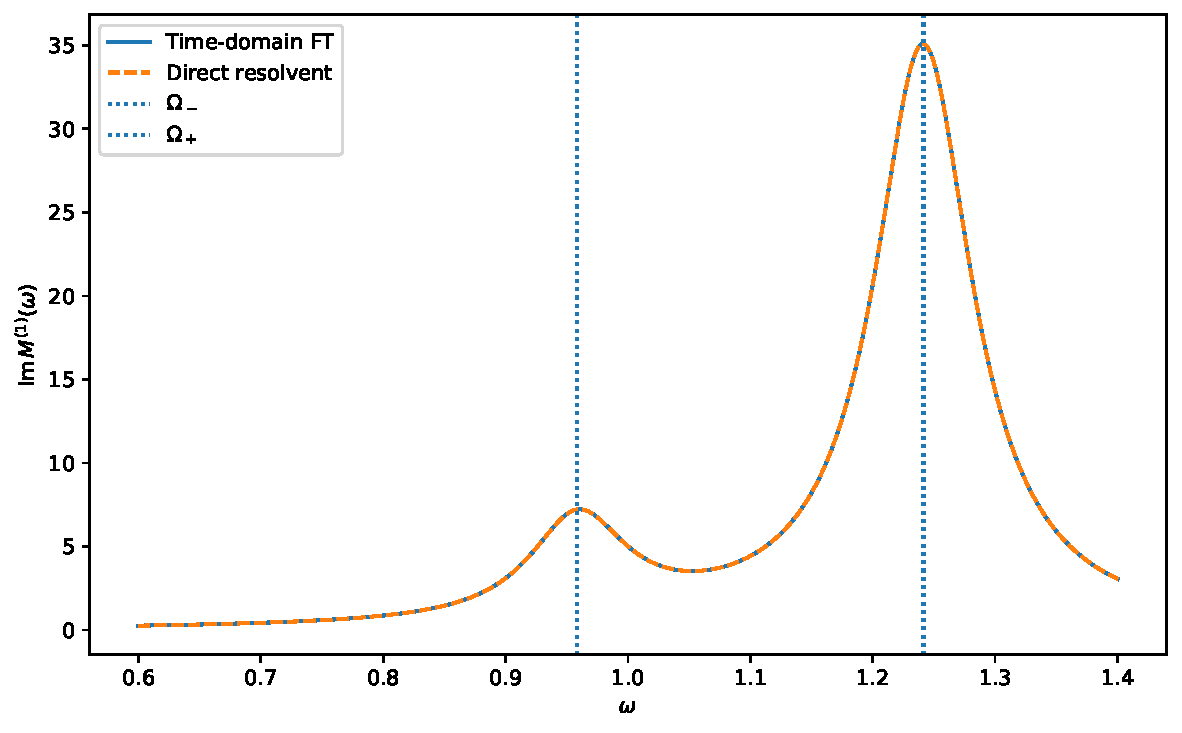
\includegraphics[
            width=\linewidth
        ]{figures/linear_impulsive_td_vs_resolvent.pdf}

        \caption{
        Imaginary part of the impulsive linear molecular response
        obtained from explicit time-domain propagation followed by
        Fourier transformation and from the direct Liouvillian
        resolvent.
        }

        \label{fig:linear_impulsive_validation}
    \end{subfigure}
    \hfill
    \begin{subfigure}[t]{0.48\textwidth}
        \centering
        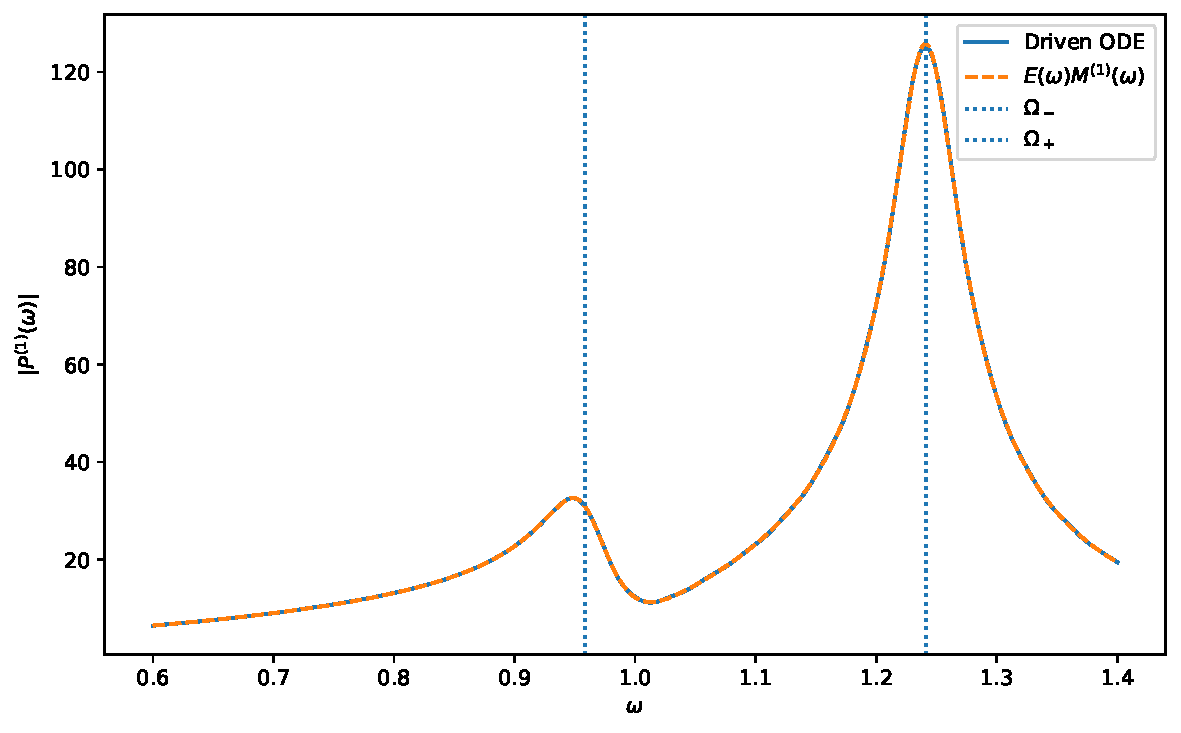
\includegraphics[
            width=\linewidth
        ]{figures/linear_stationary_finite_pulse.pdf}

        \caption{
        Magnitude of the linear polarization generated by a finite
        Gaussian pulse for the stationary preparation.  Explicit
        driven propagation is compared with
        $E(\omega)M_{\mathrm{ss}}^{(1)}(\omega)$.
        }

        \label{fig:linear_finite_pulse_validation}
    \end{subfigure}

    \caption{
    Linear-response validation of the coupled thermal dimer.
    (a) The direct Liouvillian resolvent reproduces the conventional
    time-domain propagation and Fourier-transform calculation.
    (b) For a stationary initial state, explicit propagation under a
    finite Gaussian pulse reproduces the frequency-domain
    factorization
    $P^{(1)}(\omega)=E(\omega)M^{(1)}(\omega)$.
    }

    \label{fig:linear_validation}
\end{figure}


% ============================================================
\subsubsection{Recovery of the molecular response}
% ============================================================

Equation~\eqref{eq:linear_polarization_factorization} also gives a
direct relation between the polarization generated by a known laser
pulse and the intrinsic molecular response.  Wherever the complex laser
spectrum is appreciably nonzero,
%
\begin{equation}
\boxed{
M_{\mathrm{ss}}^{(1)}(\omega)
=
\frac{
P^{(1)}(\omega)
}{
E(\omega)
}.
}
\label{eq:linear_response_deconvolution}
\end{equation}

Thus, in the stationary linear-response regime, division by the known
complex laser spectrum removes the spectral amplitude and phase of the
pulse and recovers the molecular response.

This procedure becomes ill-conditioned outside the illuminated
bandwidth, where $|E(\omega)|$ becomes small and numerical or
experimental noise would be strongly amplified.

In the short-pulse limit, the Gaussian spectrum becomes increasingly
broad.  If the pulse area is held fixed while the temporal width
approaches zero, the laser spectrum becomes approximately constant over
the molecular spectral window.  The polarization then approaches
%
\begin{equation}
P^{(1)}(\omega)
\propto
M^{(1)}(\omega),
\end{equation}
%
which is the usual impulsive-response limit.


% ============================================================
\subsubsection{Weak-field limit of the complete driven dynamics}
% ============================================================

The perturbative first-order calculation was also compared with the
complete laser-driven Lindblad equation,
%
\begin{equation}
\boxed{
\frac{d\rho}{dt}
=
-\frac{i}{\hbar}
[H_S-\mu E(t),\rho]
+
\sum_k
\mathcal{D}[L_k]\rho .
}
\label{eq:full_driven_linear_validation}
\end{equation}

Unlike Eq.~\eqref{eq:linear_driven_stationary}, this equation contains
all orders of the laser field.

For a weak field with amplitude scaling
%
\begin{equation}
E(t)
\rightarrow
\epsilon E(t),
\qquad
\epsilon=0.01,
\end{equation}
%
the polarization obtained from the complete driven equation agrees with
the perturbative first-order prediction
%
\begin{equation}
\epsilon P^{(1)}(t)
\end{equation}
%
with a relative difference of approximately
%
\begin{equation}
\boxed{
7.4\times10^{-4}.
}
\label{eq:linear_weak_field_error}
\end{equation}

This verifies that the perturbative linear-response equation is
recovered from the complete driven open-system dynamics in the
weak-field regime.


% ============================================================
\subsubsection{Nonstationary prepared ground state}
% ============================================================

Finally, we examine the effect of using the prepared ground state
%
\begin{equation}
\rho_0
=
|gg\rangle\langle gg|
\end{equation}
%
at finite thermal occupation.

In this case,
%
\begin{equation}
\mathcal{L}
|\rho_0\rangle\rangle
\neq0,
\end{equation}
%
so the zeroth-order state evolves under the thermal Liouvillian before
and during a finite first pulse.

To quantify the nonstationarity of the prepared state, we define the
norm-based initial drift scale

\begin{equation}
\boxed{
\kappa_0
=
\frac{
\left\|
\mathcal{L}
|\rho_0\rangle\rangle
\right\|_2
}{
\left\|
|\rho_0\rangle\rangle
\right\|_2
}.
}
\label{eq:initial_drift_scale}
\end{equation}

For the prepared ground state used here,

\begin{equation}
\boxed{
\kappa_0
=
0.0061237.
}
\end{equation}

The corresponding inverse scale is

\begin{equation}
\kappa_0^{-1}
\simeq
163.3.
\end{equation}

Because $\kappa_0$ is defined from the instantaneous norm of the
Liouvillian drift, $\kappa_0^{-1}$ should be regarded as a convenient
reference timescale rather than as a unique physical relaxation time.

For the Gaussian pulse used in this test,
%
\begin{equation}
\sigma
=
2,
\qquad
\tau_{\mathrm{prep}}
=
8,
\end{equation}
%
the two dimensionless diagnostics are
%
\begin{equation}
\boxed{
\chi_{\mathrm{width}}
=
\sigma\kappa_0
\simeq
0.0122,
}
\end{equation}
%
and
%
\begin{equation}
\boxed{
\chi_{\mathrm{delay}}
=
\tau_{\mathrm{prep}}\kappa_0
\simeq
0.0490.
}
\end{equation}

The exact perturbative calculation retains the evolving zeroth-order
state,
%
\begin{equation}
|\rho^{(0)}(t)\rangle\rangle
=
e^{\mathcal{L}t}
|\rho_0\rangle\rangle,
\end{equation}
%
so that
%
\begin{equation}
\frac{d}{dt}
|\rho_{\mathrm{exact}}^{(1)}(t)\rangle\rangle
=
\mathcal{L}
|\rho_{\mathrm{exact}}^{(1)}(t)\rangle\rangle
+
E^{(+)}(t)
V
|\rho^{(0)}(t)\rangle\rangle .
\label{eq:prepared_exact_linear}
\end{equation}

The frozen-preparation approximation instead replaces
%
\begin{equation}
|\rho^{(0)}(t)\rangle\rangle
\rightarrow
|\rho_0\rangle\rangle
\end{equation}
%
during the first interaction.

For the present pulse parameters, the exact and frozen calculations
differ by approximately
%
\begin{equation}
\boxed{
4.45\%
}
\end{equation}
%
in the time domain and
%
\begin{equation}
\boxed{
4.46\%
}
\end{equation}
%
in the frequency domain.

By contrast, the frozen-state propagation agrees with the factorized
frequency-domain result
%
\begin{equation}
E^{(+)}(\omega)
M_{\rho_0}^{(1)}(\omega)
\end{equation}
%
to approximately
%
\begin{equation}
\boxed{
0.42\%.
}
\end{equation}

The corresponding spectral comparison is shown in
Fig.~\ref{fig:linear_prepared_state}.


% ============================================================
% PREPARED-STATE FIGURE
% ============================================================

\begin{figure}[htbp]
    \centering

    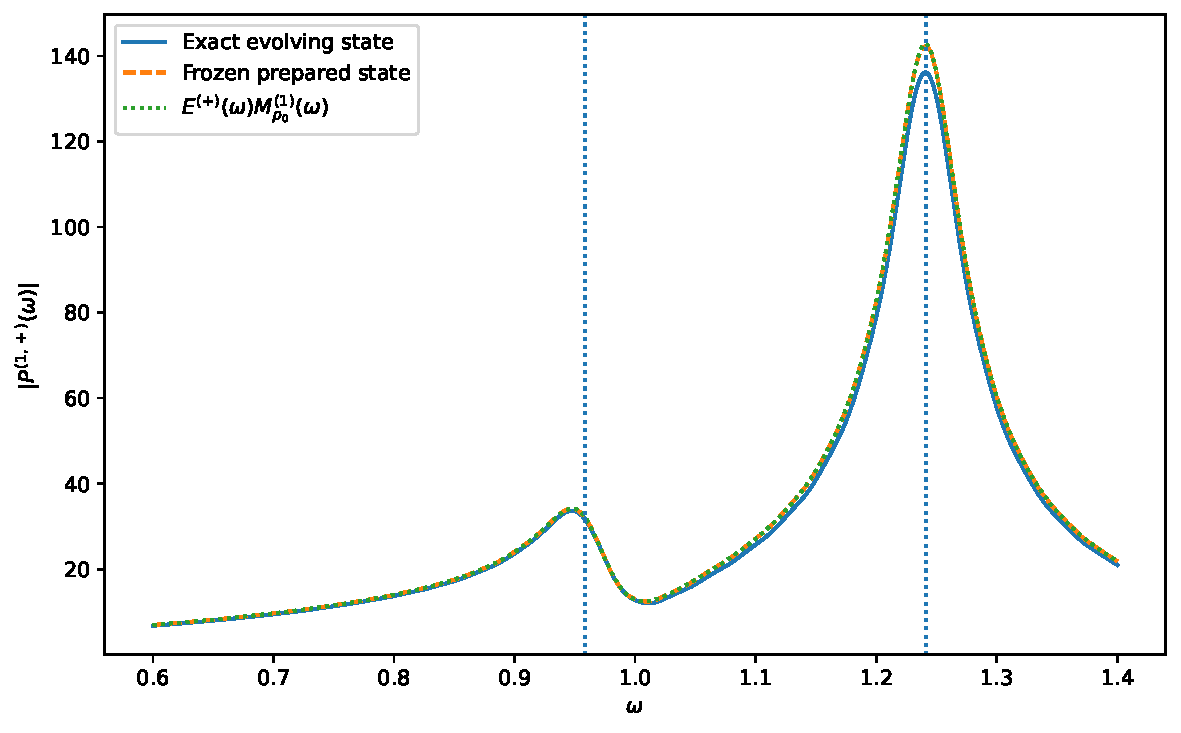
\includegraphics[
        width=0.72\textwidth
    ]{figures/linear_prepared_state_comparison.pdf}

    \caption{
    Linear finite-pulse response for the nonstationary prepared ground
    state.  The exact calculation retains the field-free evolution of
    the zeroth-order state before and during the laser pulse.  The
    frozen-preparation calculation neglects this evolution and closely
    agrees with the factorized frequency-domain result
    $E^{(+)}(\omega)M_{\rho_0}^{(1)}(\omega)$.  The remaining difference
    between the exact and frozen calculations originates from the
    nonstationary evolution of the prepared initial state.
    }

    \label{fig:linear_prepared_state}
\end{figure}


The agreement between the frozen propagation and the factorized
frequency-domain expression shows that the approximately $4.5\%$
difference in the exact calculation does not originate from the
resolvent formulation.  Instead, it results from the field-free
evolution of the nonstationary prepared state before and during the
pulse.

For this parameter set,

\begin{equation}
\chi_{\mathrm{delay}}
>
\chi_{\mathrm{width}},
\end{equation}

so the larger accumulated drift scale is associated with the
preparation-to-pulse delay. This is consistent with the delay playing
a larger role in the observed discrepancy than evolution across the
pulse width alone. The quantities $\chi_{\mathrm{delay}}$ and
$\chi_{\mathrm{width}}$ are diagnostic scales and should not be
interpreted as quantitative error estimates.


% ============================================================
\subsubsection{Summary of the linear validation}
% ============================================================

The linear-response calculations establish the following numerical
consistency chain:
%
\begin{equation}
\boxed{
\begin{gathered}
\text{direct Lindblad propagation}
\\
\Updownarrow
\\
\text{Liouville-space propagation}
\\
\Updownarrow
\\
\text{time-domain molecular response}
\\
\Updownarrow
\\
\text{direct Liouvillian resolvent}
\\
\Updownarrow
\\
\text{finite-pulse polarization}.
\end{gathered}
}
\end{equation}

The agreement across these independent calculations validates the
Liouvillian construction, the direct frequency-domain linear response,
the finite-pulse convolution for a stationary preparation, and the
treatment of a nonstationary prepared state.  These results provide the
numerical foundation for the third-order validation developed next.

% ============================================================
\subsection{Impulsive Third-Order Validation}
\label{subsec:third_order_impulsive}
% ============================================================

We next validate the direct frequency-domain construction at third
order.  We begin in the impulsive limit, in which the three optical
interactions occur at well-defined times and the temporal widths of the
laser pulses are neglected.

The validation is performed in three stages.  First, the direct
frequency-domain resolvent expression is compared with an explicit
two-dimensional time-domain propagation using the complete interaction
superoperator $V$.  This test is independent of the rotating-wave
approximation.  Second, the interaction is decomposed into
excitation-raising and excitation-lowering components to construct the
conventional rephasing and nonrephasing RWA responses.  Finally, these
RWA-resolved responses are compared with an independent QuDPy
time-domain pathway calculation.


% ============================================================
\subsubsection{Full-interaction time-domain and resolvent equivalence}
% ============================================================

For three impulsive interactions separated by the coherence time
$t_1$, waiting time $T$, and detection time $t_3$, the complete
third-order molecular response is

\begin{equation}
R^{(3)}(t_3,T,t_1)
=
\langle\!\langle \mu |
e^{\mathcal{L}t_3}
V
e^{\mathcal{L}T}
V
e^{\mathcal{L}t_1}
V
|\rho_0\rangle\!\rangle ,
\label{eq:third_order_impulsive_td}
\end{equation}

where

\begin{equation}
V
=
\frac{i}{\hbar}
\left(
I\otimes\mu-\mu^{T}\otimes I
\right)
\end{equation}

is the complete dipole interaction superoperator.

Using the causal Fourier convention

\begin{equation}
f(\omega)
=
\int_0^\infty dt\,
e^{+i\omega t}f(t),
\end{equation}

together with a small positive damping parameter $\eta$, we define the
numerical Liouvillian resolvent

\begin{equation}
G_\eta(\omega)
=
\left[
(\eta-i\omega)I-\mathcal{L}
\right]^{-1}.
\label{eq:liouvillian_resolvent}
\end{equation}

The corresponding mixed frequency--time--frequency response can then
be evaluated directly as

\begin{equation}
M^{(3)}(\omega_3,T,\omega_1)
=
\langle\!\langle\mu|
G_\eta(\omega_3)
V
e^{\mathcal{L}T}
V
G_\eta(\omega_1)
V
|\rho_0\rangle\!\rangle .
\label{eq:third_order_impulsive_fd}
\end{equation}

Equation~\eqref{eq:third_order_impulsive_fd} replaces explicit
propagation along the two coherence-time coordinates by two
Liouvillian resolvent evaluations.  Numerically, the action of each
resolvent is obtained by solving the corresponding linear system rather
than constructing the matrix inverse explicitly.

To verify this construction independently, we calculated
$R^{(3)}(t_3,T,t_1)$ directly on a two-dimensional time grid and
performed the damped transform

\begin{equation}
M_{\mathrm{TD}}^{(3)}
(\omega_3,T,\omega_1)
=
\int_0^\infty dt_3
\int_0^\infty dt_1\,
e^{(i\omega_3-\eta)t_3}
e^{(i\omega_1-\eta)t_1}
R^{(3)}(t_3,T,t_1).
\label{eq:third_order_td_transform}
\end{equation}

The transformed time-domain response was compared point by point with
the direct resolvent result.  We quantify the discrepancy using the
Frobenius norm of the complete complex two-dimensional spectra,

\begin{equation}
\epsilon_{\mathrm{TD/FD}}
=
\frac{
\left\|
M_{\mathrm{TD}}^{(3)}
-
M_{\mathrm{FD}}^{(3)}
\right\|_F
}{
\left\|
M_{\mathrm{FD}}^{(3)}
\right\|_F
}.
\label{eq:third_order_td_fd_error}
\end{equation}

For the coupled dimer considered here,

\begin{equation}
\boxed{
\epsilon_{\mathrm{TD/FD}}
\simeq
5.4\times10^{-5}.
}
\end{equation}

The agreement demonstrates the numerical equivalence between explicit
causal propagation followed by a two-dimensional Fourier transform and
direct evaluation through the Liouvillian resolvent.

Importantly, the complete interaction superoperator $V$ is retained
throughout this comparison.  The result therefore validates the direct
frequency-domain construction itself before any molecular
rotating-wave approximation or pathway selection is introduced.

\begin{figure}[htbp]
    \centering

    \begin{minipage}{0.32\textwidth}
        \centering
        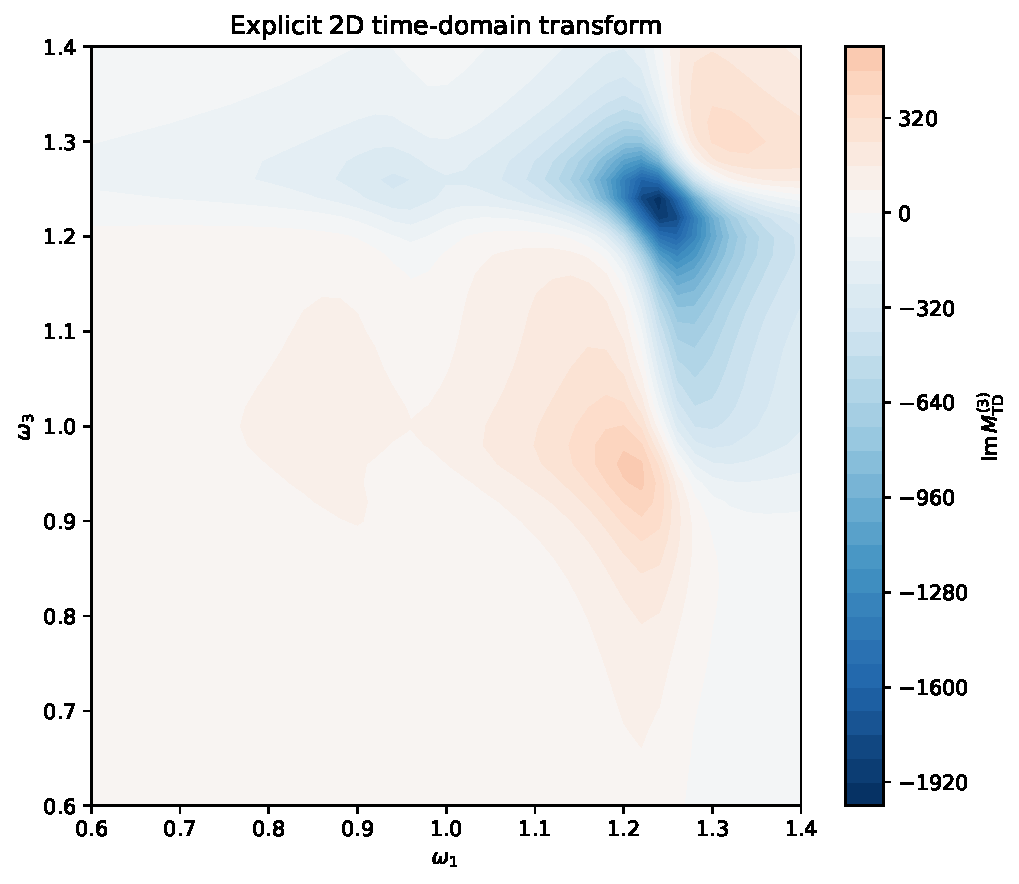
\includegraphics[width=\linewidth]{figures/third_order_impulsive_td.pdf}
    \end{minipage}
    \hfill
    \begin{minipage}{0.32\textwidth}
        \centering
        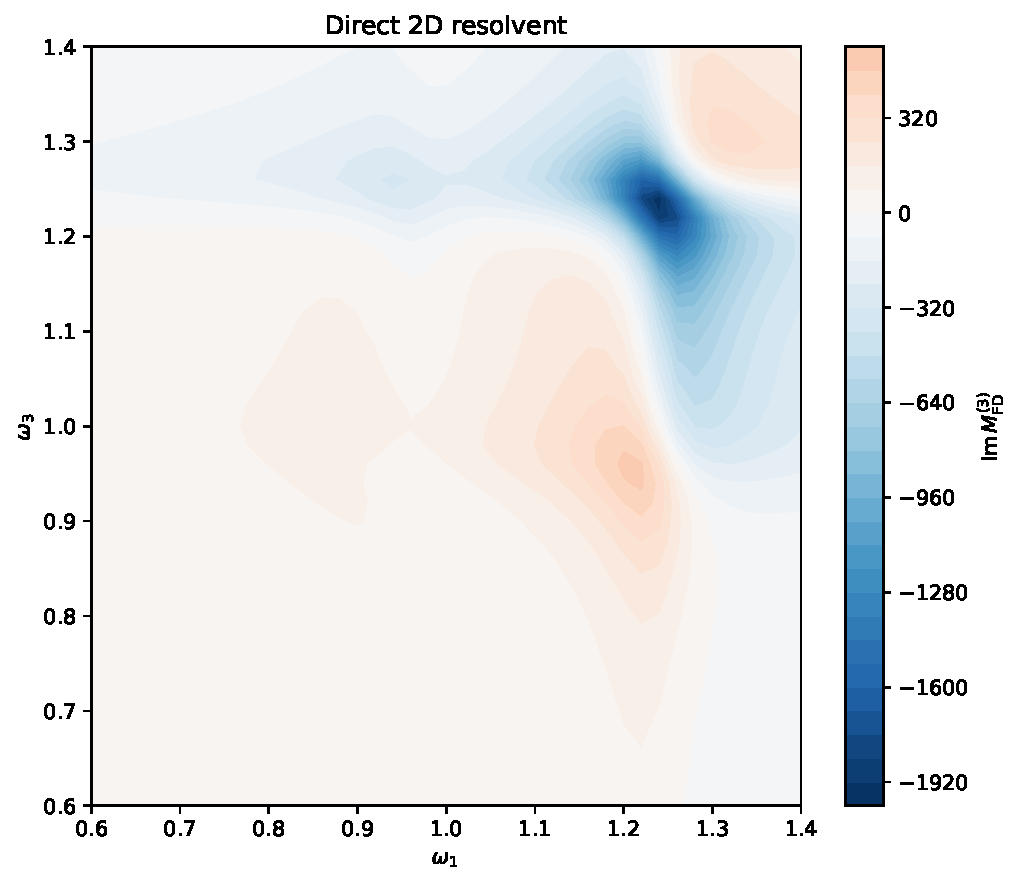
\includegraphics[width=\linewidth]{figures/third_order_direct_2d_resolvent.pdf}
    \end{minipage}
    \hfill
    \begin{minipage}{0.32\textwidth}
        \centering
        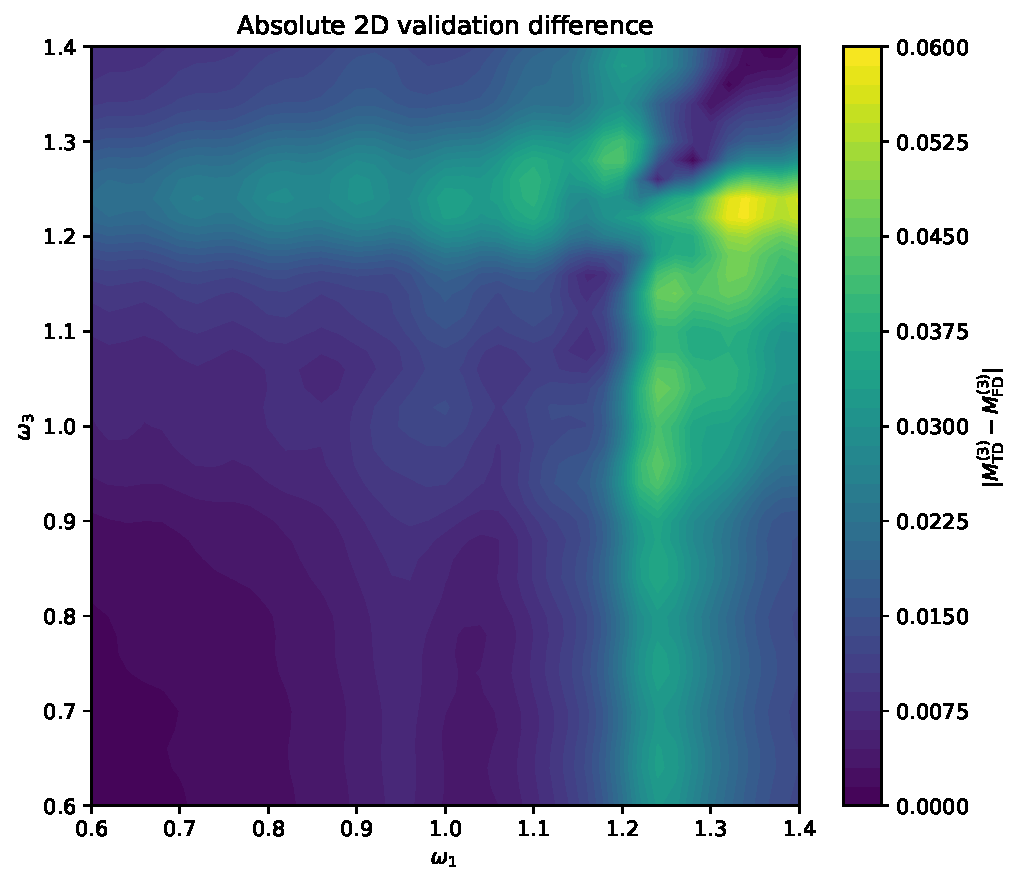
\includegraphics[width=\linewidth]{figures/third_order_2d_validation_difference.pdf}
    \end{minipage}

    \caption{
    Comparison of the impulsive full-interaction third-order spectrum
    obtained from explicit two-dimensional time-domain propagation and
    Fourier transformation (left), direct Liouvillian-resolvent
    evaluation (center), and their difference (right).
    The relative complex two-dimensional discrepancy is
    $\epsilon_{\mathrm{TD/FD}}\simeq5.4\times10^{-5}$.
    }

    \label{fig:third_order_td_vs_resolvent}
\end{figure}


% ============================================================
\subsubsection{RWA-resolved rephasing and nonrephasing response}
% ============================================================

Having validated the direct resolvent formulation using the complete
interaction superoperator, we next introduce the rotating-wave
decomposition required for the conventional impulsive rephasing and
nonrephasing signals.

The dipole operator is decomposed into excitation-raising and
excitation-lowering components,

\begin{equation}
\mu
=
\mu_{\uparrow}
+
\mu_{\downarrow},
\qquad
\mu_{\downarrow}
=
\mu_{\uparrow}^{\dagger}.
\end{equation}

The corresponding interaction superoperators are

\begin{equation}
V_{\uparrow}
=
\frac{i}{\hbar}
\left(
I\otimes\mu_{\uparrow}
-
\mu_{\uparrow}^{T}\otimes I
\right),
\end{equation}

and

\begin{equation}
V_{\downarrow}
=
\frac{i}{\hbar}
\left(
I\otimes\mu_{\downarrow}
-
\mu_{\downarrow}^{T}\otimes I
\right).
\end{equation}

For a positive-frequency optical field component,

\begin{equation}
E^{(+)}(t)
\propto
e^{-i\omega_L t},
\end{equation}

the rotating-wave approximation associates $E^{(+)}$ with
$\mu_{\uparrow}$ and $E^{(-)}$ with $\mu_{\downarrow}$.

Using the coherence-order convention in which $V_{\uparrow}$ increases
the optical coherence order by one and $V_{\downarrow}$ decreases it
by one, the positive-frequency nonrephasing field signature

\begin{equation}
(+,-,+)
\end{equation}

gives the molecular sequence
$V_{\uparrow}V_{\downarrow}V_{\uparrow}$ in chronological order.
The corresponding response is

\begin{equation}
M_{NR}^{(3)}
(\omega_3,T,\omega_1)
=
\langle\!\langle\mu|
G_\eta(\omega_3)
V_{\uparrow}
e^{\mathcal{L}T}
V_{\downarrow}
G_\eta(\omega_1)
V_{\uparrow}
|\rho_0\rangle\!\rangle ,
\label{eq:M3_NR}
\end{equation}

with

\begin{equation}
\omega_1>0.
\end{equation}

The rephasing field signature

\begin{equation}
(-,+,+)
\end{equation}

instead gives the chronological molecular sequence
$V_{\downarrow}V_{\uparrow}V_{\uparrow}$ and the response

\begin{equation}
M_R^{(3)}
(\omega_3,T,\nu_1)
=
\langle\!\langle\mu|
G_\eta(\omega_3)
V_{\uparrow}
e^{\mathcal{L}T}
V_{\uparrow}
G_\eta(\nu_1)
V_{\downarrow}
|\rho_0\rangle\!\rangle ,
\label{eq:M3_R}
\end{equation}

where the signed first coherence frequency satisfies

\begin{equation}
\nu_1<0
\end{equation}

under the Fourier convention adopted here.

For an initial state with zero optical coherence order, both branches
return to the population sector after the second interaction and end in
the positive-frequency optical-coherence sector after the third
interaction.  The complete detection operator
$\langle\!\langle\mu|$ therefore selects the physically allowed final
coherence automatically.

For the dimer benchmark at $T=5$, the strongest features occur near the
upper excitonic transition.  The dominant nonrephasing feature lies
approximately at

\begin{equation}
(\omega_1,\omega_3)
\simeq
(1.24,1.24),
\end{equation}

while the corresponding rephasing feature appears at

\begin{equation}
(\nu_1,\omega_3)
\simeq
(-1.24,1.24).
\end{equation}

The sign reversal of the raw first-frequency axis is therefore a direct
consequence of the Fourier and field-sign conventions and not an
independent change in the molecular transition frequency.

\begin{figure}[htbp]
    \centering

    \begin{minipage}{0.48\textwidth}
        \centering
        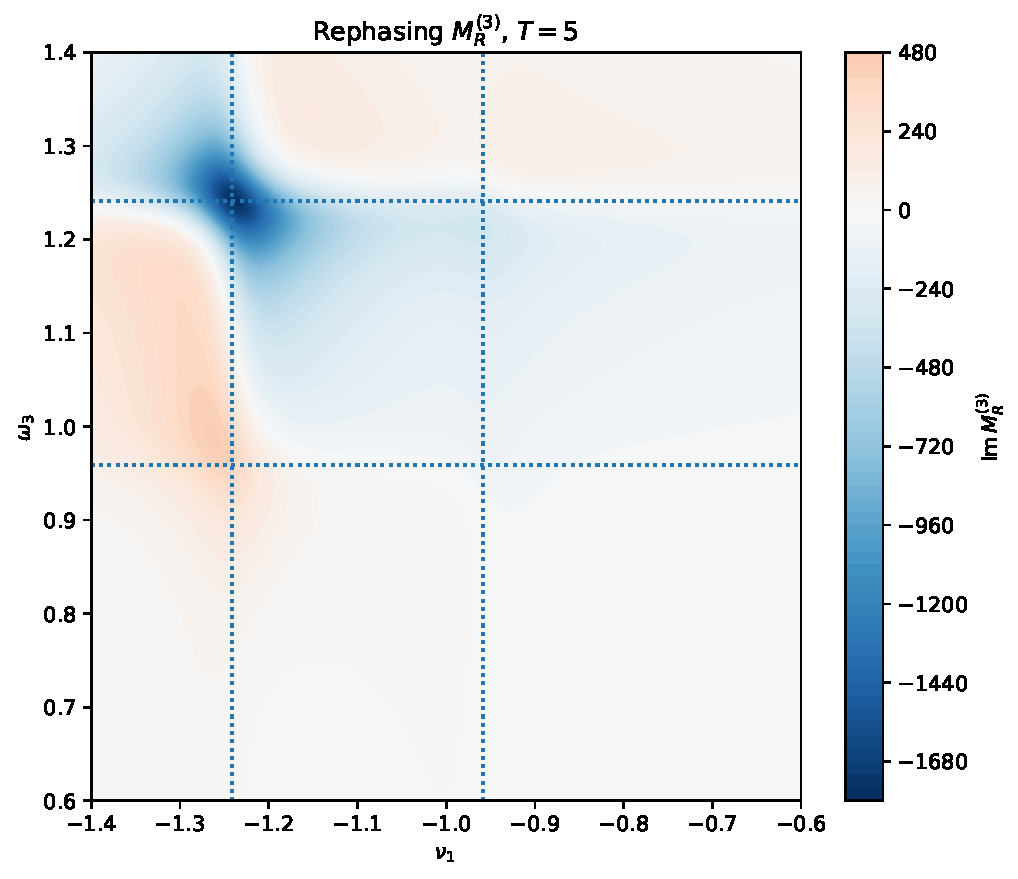
\includegraphics[width=\linewidth]{figures/third_order_impulsive_rephasing.pdf}
    \end{minipage}
    \hfill
    \begin{minipage}{0.48\textwidth}
        \centering
        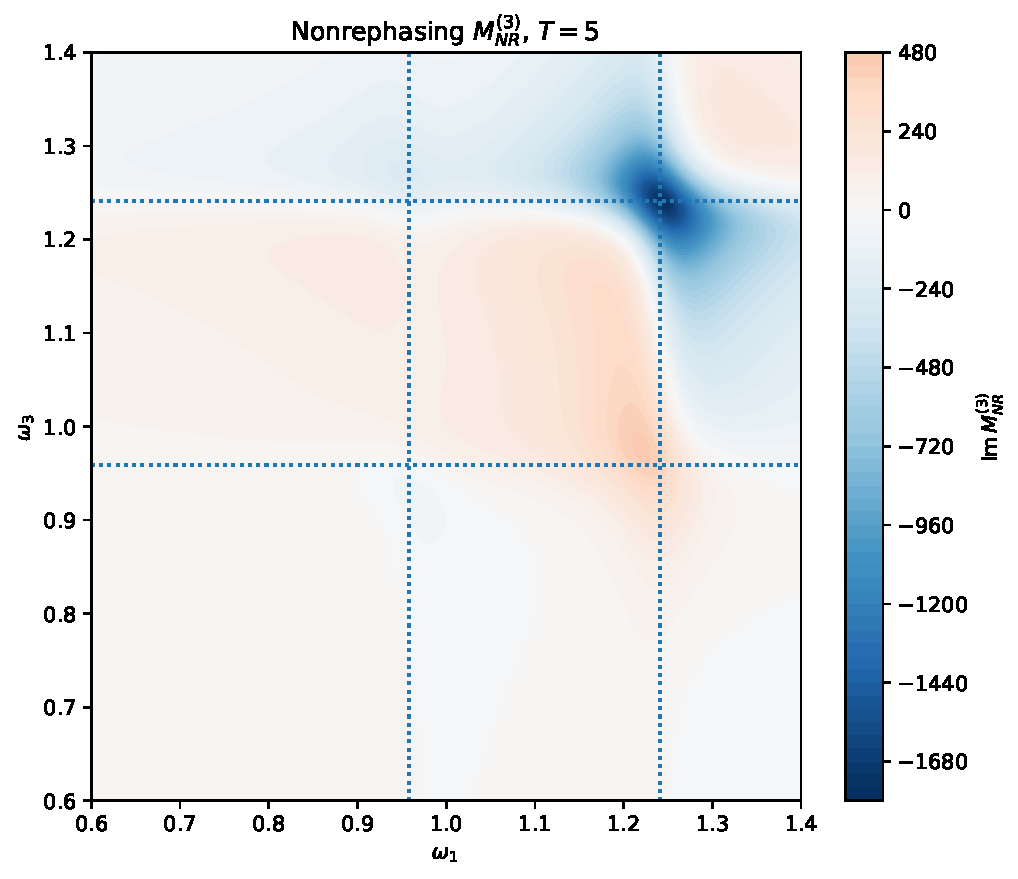
\includegraphics[width=\linewidth]{figures/third_order_impulsive_nonrephasing.pdf}
    \end{minipage}

    \caption{
    Impulsive rephasing (left) and nonrephasing (right) third-order
    spectra obtained directly from the RWA-resolved Liouvillian
    resolvent at $T=5$.
    Under the Fourier convention used here, the raw first-frequency
    axis is negative for the rephasing branch and positive for the
    nonrephasing branch.
    }

    \label{fig:third_order_impulsive_rnr}
\end{figure}


% ============================================================
\subsubsection{Independent validation against QuDPy}
% ============================================================

As an independent validation of the RWA-resolved third-order
calculation, we also evaluated the same dimer response using the
time-domain pathway propagation implemented in
QuDPy~\cite{shah2023qudpy}.

QuDPy represents the individual left- and right-acting dipole
interactions through the operations

\begin{equation}
K_u\rho
=
\mu_{\uparrow}\rho,
\qquad
B_d\rho
=
\rho\mu_{\uparrow},
\end{equation}

and

\begin{equation}
K_d\rho
=
\mu_{\downarrow}\rho,
\qquad
B_u\rho
=
\rho\mu_{\downarrow}.
\end{equation}

The RWA interaction superoperators can therefore be written as

\begin{equation}
V_{\uparrow}
=
\frac{i}{\hbar}
(K_u-B_d),
\qquad
V_{\downarrow}
=
\frac{i}{\hbar}
(K_d-B_u).
\label{eq:qudpy_commutator_connection}
\end{equation}

For this benchmark we use the ground-state preparation

\begin{equation}
\rho_0
=
|gg\rangle\langle gg|,
\end{equation}

for which the conventional three rephasing and three nonrephasing
double-sided pathways provide the complete impulsive RWA response.

With $\hbar=1$, expansion of the commutator superoperators gives

\begin{equation}
R_R^{(3)}
=
i
\left(
R_3-R_1-R_2
\right),
\label{eq:qudpy_rephasing_combination}
\end{equation}

and

\begin{equation}
R_{NR}^{(3)}
=
i
\left(
R_4-R_5-R_6
\right).
\label{eq:qudpy_nonrephasing_combination}
\end{equation}

The individual QuDPy pathways were propagated explicitly in time.
Rather than using the built-in QuDPy Fourier-transform and plotting
conventions, the resulting complex time-domain responses were
transformed using the same damped causal Fourier convention as
Eq.~\eqref{eq:third_order_td_transform}.  This isolates differences in
the underlying dynamical implementations from differences caused by
FFT signs, axis conventions, or plotting conventions.

Using a QuDPy propagation window of

\begin{equation}
t_{\max}=100
\end{equation}

and a temporal spacing of approximately

\begin{equation}
\Delta t=0.251,
\end{equation}

the complete complex spectra give relative discrepancies

\begin{equation}
\epsilon_{NR}
=
1.45\times10^{-2},
\end{equation}

and

\begin{equation}
\epsilon_R
=
1.43\times10^{-2}.
\end{equation}

No amplitude normalization or global phase adjustment was applied in
these comparisons.

As an additional diagnostic, we allow the direct frequency-domain
spectrum to acquire a single optimal global complex factor before
comparison with the QuDPy result. We define

\begin{equation}
\alpha_{\mathrm{FD}\rightarrow\mathrm{Q}}
=
\frac{
\sum_{i,j}
\left(
M_{\mathrm{FD},ij}^{(3)}
\right)^*
M_{\mathrm{Q},ij}^{(3)}
}{
\sum_{i,j}
\left|
M_{\mathrm{FD},ij}^{(3)}
\right|^2
}.
\label{eq:qudpy_alpha_opt}
\end{equation}

With this convention,

\begin{equation}
\alpha_{NR}
=
1.0075+0.0019i,
\end{equation}

and

\begin{equation}
\alpha_R
=
1.0069-0.0021i.
\end{equation}

Both are close to unity. After removing these small global amplitude
and phase differences only as a diagnostic, the remaining
spectral-shape discrepancies are approximately $1.22\%$ for the
nonrephasing branch and $1.23\%$ for the rephasing branch.


The agreement verifies the connection between the direct
Liouville-space commutator formulation and the conventional
double-sided pathway construction.  In particular, it independently
checks the RWA interaction signs, the mapping of left- and right-acting
dipole operations, and the rephasing/nonrephasing decomposition.

\begin{figure}[htbp]
    \centering

    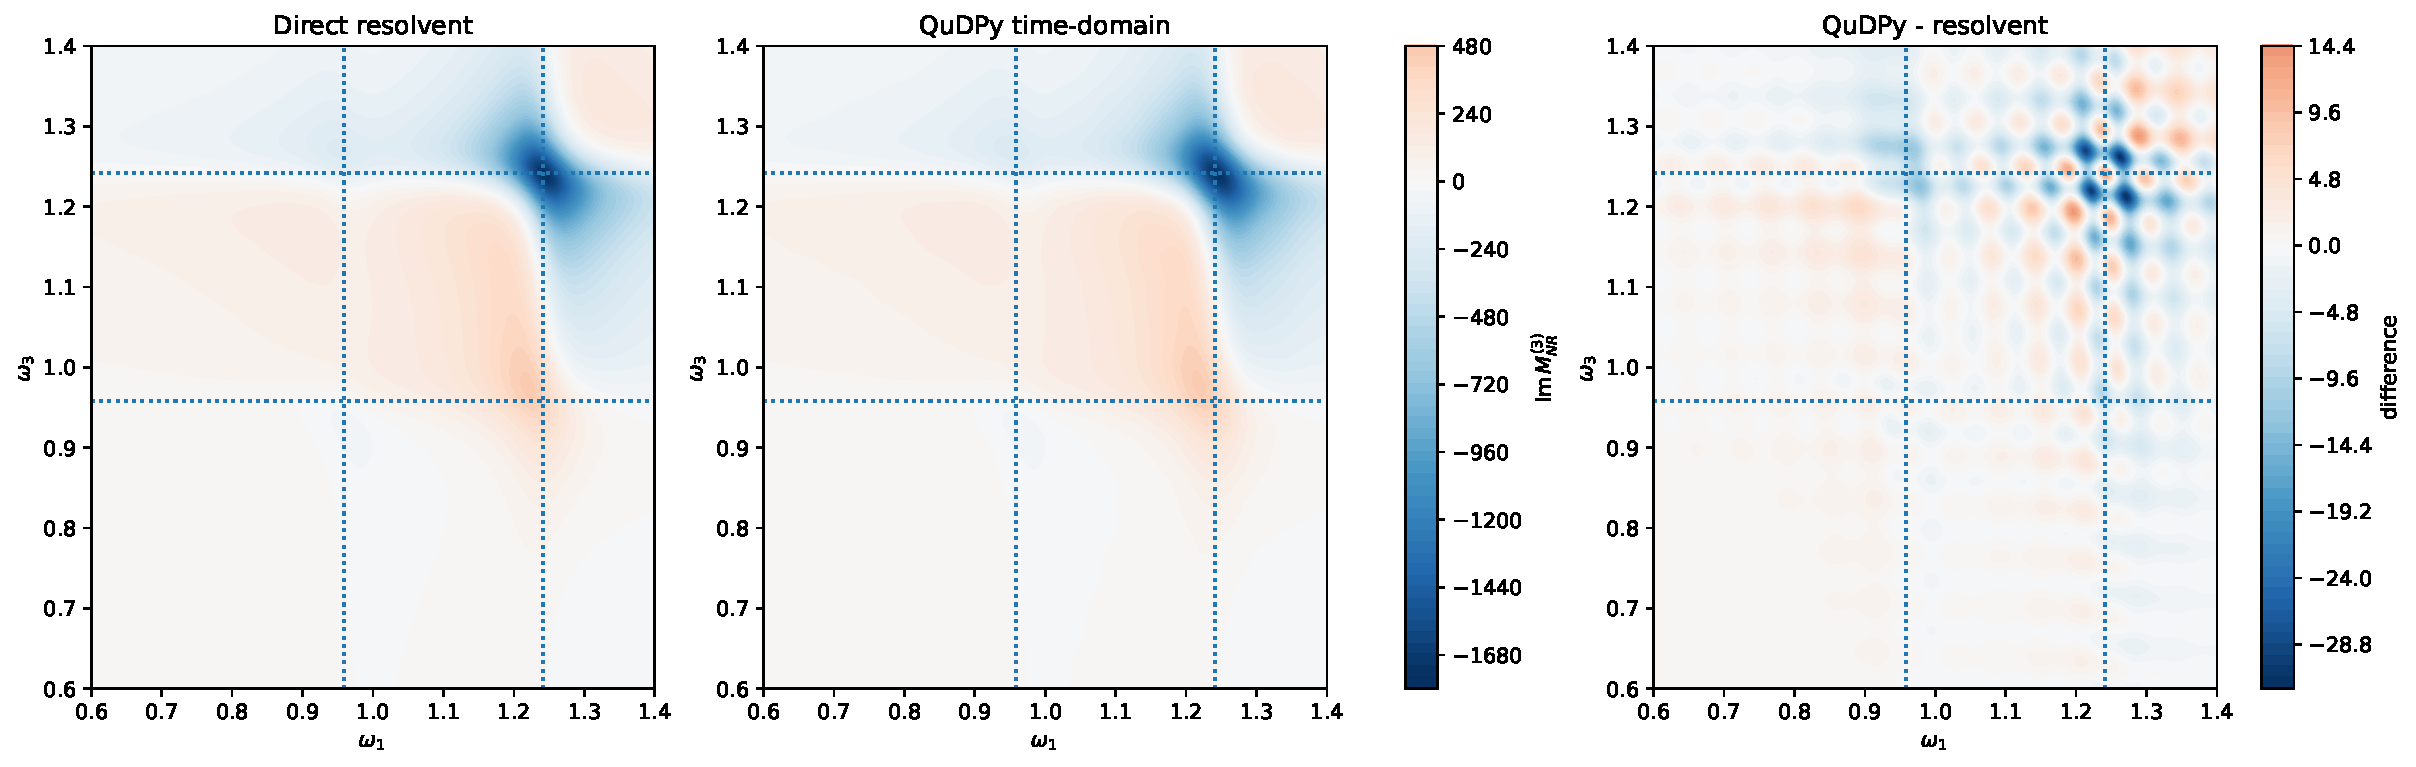
\includegraphics[width=0.98\textwidth]{figures/third_order_qudpy_nonrephasing_comparison.pdf}

    \vspace{0.5em}

    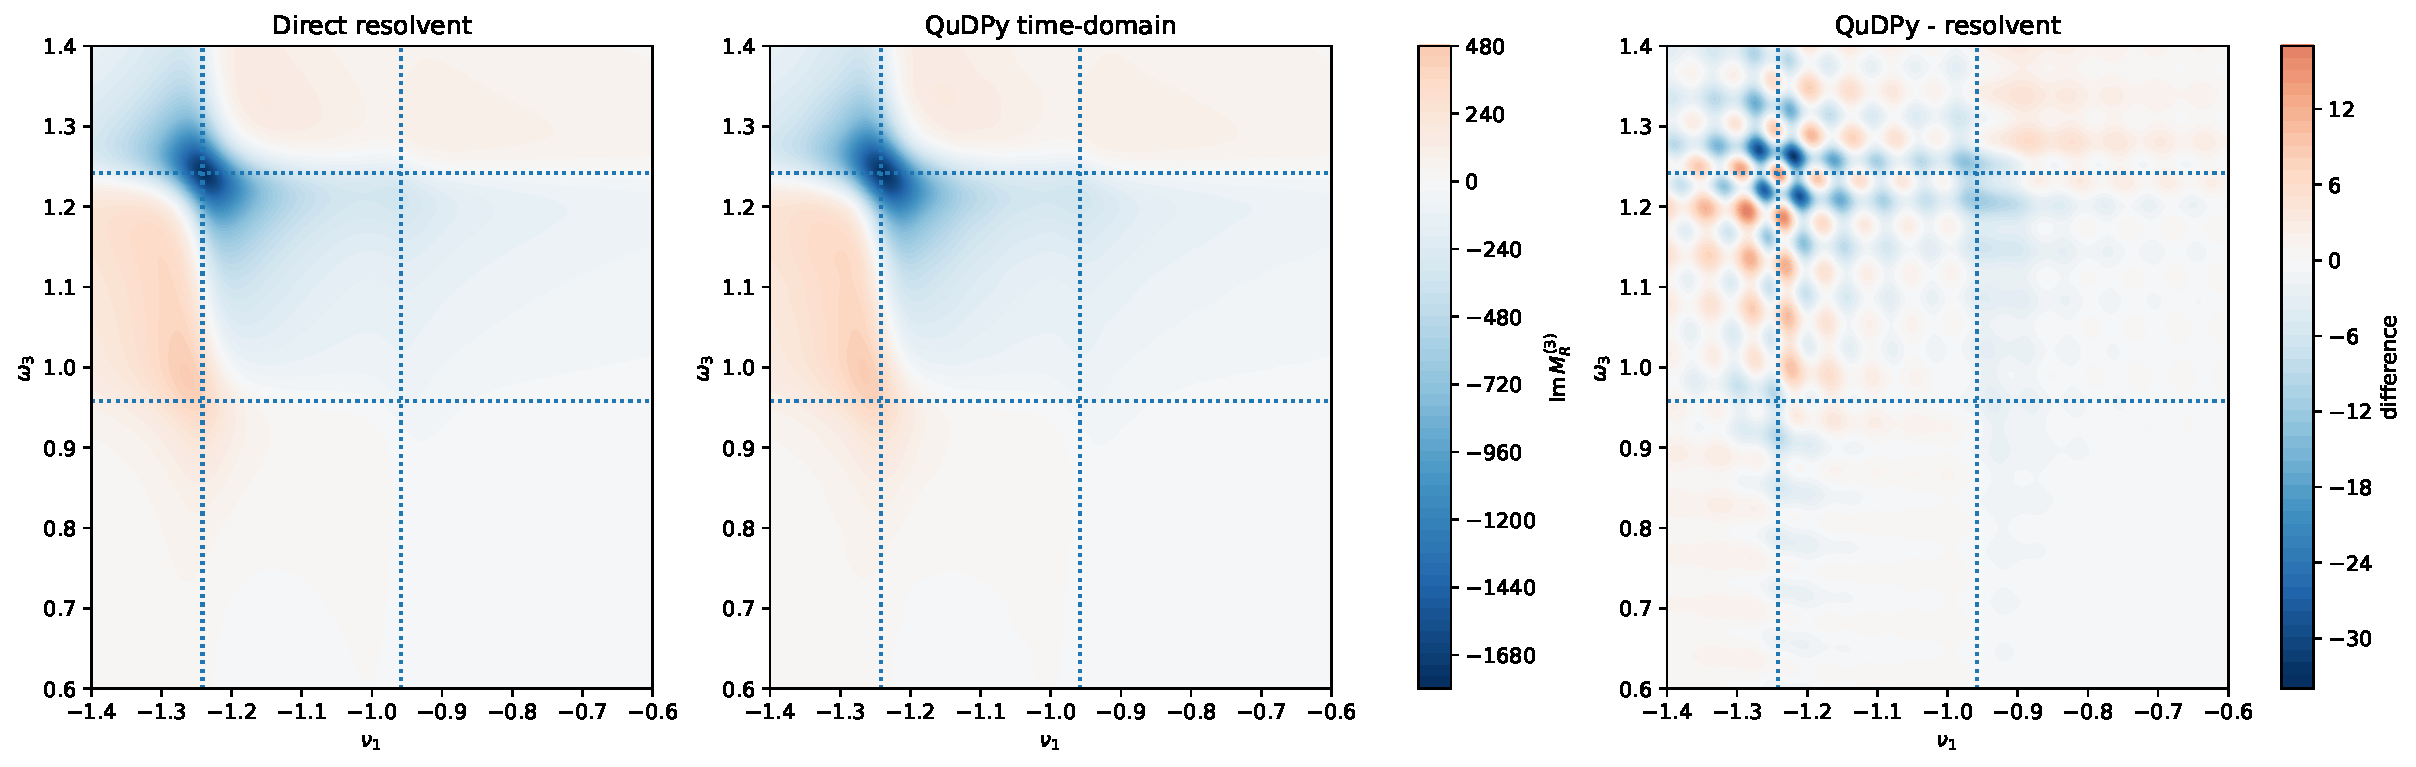
\includegraphics[width=0.98\textwidth]{figures/third_order_qudpy_rephasing_comparison.pdf}

    \caption{
    Independent comparison of the direct frequency-domain RWA
    resolvent calculation with explicit QuDPy time-domain pathway
    propagation.
    The upper row shows the nonrephasing response and the lower row the
    rephasing response.
    Within each row, the panels show the direct resolvent result, the
    QuDPy time-domain result transformed using the same Fourier
    convention, and their difference.
    No amplitude normalization or phase correction was applied.
    The full complex two-dimensional relative discrepancies are
    $1.45\%$ and $1.43\%$ for the nonrephasing and rephasing branches,
    respectively.
    }

    \label{fig:third_order_qudpy_validation}
\end{figure}

% ============================================================
\subsection{Finite-Width Third-Order Validation}
\label{subsec:third_order_finite_width}
% ============================================================

Having validated the impulsive third-order resolvent formulation and its
RWA-resolved implementation, we now introduce finite pulse durations.
The purpose of this subsection is to test the operator-valued
finite-pulse construction, quantify the accuracy of the conventional
short-pulse approximation, and determine the temporal-separation regime
in which the finite-width factorization remains valid.

For these calculations we use the stationary state of the thermal
Liouvillian,

\begin{equation}
\mathcal{L}
|\rho_{\mathrm{ss}}\rangle\rangle
=
0,
\end{equation}

as the initial preparation unless stated otherwise.

The finite-width calculation retains the complete dipole interaction
superoperator

\begin{equation}
V
=
V_{\uparrow}
+
V_{\downarrow}
\end{equation}

at every interaction.  Thus, unlike the conventional impulsive RWA
calculation of Sec.~\ref{subsec:third_order_impulsive}, no
excitation-raising or excitation-lowering molecular pathway is imposed
by hand.


% ============================================================
\subsubsection{Finite-pulse operators and short-pulse reference}
% ============================================================

For a selected field-signature branch
$\mathbf{s}=(s_1,s_2,s_3)$, the finite-width frequency-domain response is

\begin{equation}
\boxed{
\begin{aligned}
P_{\mathbf{s},\mathrm{finite}}^{(3)}
(\omega_3,T,\omega_1)
=
\langle\!\langle\mu|
&G_\eta(\omega_3)
V
e^{\mathcal{L}T}
F_3^{(s_3)}(\omega_3)
F_2^{(s_2)}(\omega_1)
\\
&\times
V
G_\eta(\omega_1)
V
F_1^{(s_1)}(\omega_1)
|\rho_{\mathrm{ss}}\rangle\rangle .
\end{aligned}
}
\label{eq:third_order_finite_validation}
\end{equation}

with the signed first coherence frequency used for the rephasing
branch as described in Sec.~\ref{subsec:third_order_impulsive}.

The nonrephasing field signature is

\begin{equation}
(s_1,s_2,s_3)
=
(+,-,+),
\end{equation}

whereas the rephasing branch uses

\begin{equation}
(s_1,s_2,s_3)
=
(-,+,+).
\end{equation}

The operators $F_1$, $F_2$, and $F_3$ incorporate both the Gaussian
pulse spectra and the field-free Liouvillian evolution occurring over
the pulse offsets.  Their closed forms were derived in
Sec.~\ref{sec:finite_pulses}.

As a first numerical test, the analytical matrix-exponential forms of
all three finite-pulse operators were compared with direct numerical
evaluation of their defining time integrals.  The relative differences
were of order

\begin{equation}
10^{-13},
\end{equation}

confirming the numerical implementation of the Gaussian
Liouvillian-dressing operators.

For the stationary preparation, the first pulse operator must satisfy

\begin{equation}
F_1^{(s_1)}
|\rho_{\mathrm{ss}}\rangle\rangle
=
E_1^{(s_1)}
|\rho_{\mathrm{ss}}\rangle\rangle .
\label{eq:third_order_stationary_F1_identity}
\end{equation}

Numerically, this identity is satisfied to a relative difference of
approximately

\begin{equation}
2\times10^{-16}.
\end{equation}

Although $F_1$ therefore reduces to a scalar spectral factor for this
particular preparation, the complete $F_1F_2F_3$ structure is retained
in the implementation so that the same formulation can be applied to
nonstationary initial states.

For comparison, the conventional short-pulse RWA approximation
neglects molecular evolution during the pulse offsets and retains only
scalar laser spectra multiplying the impulsive RWA molecular response,

\begin{equation}
P_{s,\mathrm{short}}^{(3)}
=
E_3^{(s_3)}
E_2^{(s_2)}
E_1^{(s_1)}
M_s^{(3)}.
\label{eq:third_order_short_validation}
\end{equation}

The impulsive RWA response is recovered by removing these finite
spectral envelope factors.  The finite-width, short-pulse RWA, and
impulsive RWA calculations therefore provide a hierarchy in which the
effects of finite pulse duration and the rotating-wave approximation
can be distinguished numerically.


% ============================================================
\subsubsection{Explicit finite-pulse ODE benchmark}
% ============================================================

The finite-width frequency-domain formulation was benchmarked against
an independent perturbative time-domain calculation with explicit
Gaussian laser pulses.

For a selected field signature, the sequential third-order hierarchy is

\begin{align}
\frac{d}{dt}
|\rho^{(1)}\rangle\rangle
&=
\mathcal{L}
|\rho^{(1)}\rangle\rangle
+
E_1^{(s_1)}(t)
V
|\rho_{\mathrm{ss}}\rangle\rangle ,
\\
\frac{d}{dt}
|\rho^{(2)}\rangle\rangle
&=
\mathcal{L}
|\rho^{(2)}\rangle\rangle
+
E_2^{(s_2)}(t)
V
|\rho^{(1)}\rangle\rangle ,
\\
\frac{d}{dt}
|\rho^{(3)}\rangle\rangle
&=
\mathcal{L}
|\rho^{(3)}\rangle\rangle
+
E_3^{(s_3)}(t)
V
|\rho^{(2)}\rangle\rangle .
\label{eq:third_order_finite_ode}
\end{align}

The complete interaction superoperator $V$ is used at every order.
Consequently, this benchmark does not impose a molecular
rotating-wave approximation.

The pulse-center variables were transformed over a nearly bilateral
numerical domain so that the time-domain benchmark implements the same
translation-invariant Fourier construction used in the analytical
finite-width derivation.  A common damping parameter $\eta$ was
included consistently in the numerical Fourier transform, the
resolvents, and the finite-$\eta$ versions of the pulse operators.
This modification is used only to make the finite numerical transform
and frequency-domain calculation directly comparable; the physical
expressions correspond to the limit $\eta\rightarrow0^{+}$.

To compare complete complex spectra we use the Frobenius norm,

\begin{equation}
\|P\|_F
=
\left[
\sum_{i,j}
|P_{ij}|^2
\right]^{1/2}.
\end{equation}

When different approximations contain different overall pulse
prefactors, it is also useful to separate a global complex amplitude
and phase difference from a change in spectral structure.  We therefore
define

\begin{equation}
\alpha_{\mathrm{opt}}
=
\frac{
\sum_{i,j}
P_{\mathrm{model},ij}^{*}
P_{\mathrm{ODE},ij}
}{
\sum_{i,j}
|P_{\mathrm{model},ij}|^2
},
\label{eq:third_order_alpha_opt}
\end{equation}

and the corresponding spectral-shape discrepancy

\begin{equation}
\epsilon_{\mathrm{shape}}
=
\frac{
\|
\alpha_{\mathrm{opt}}
P_{\mathrm{model}}
-
P_{\mathrm{ODE}}
\|_F
}{
\|
P_{\mathrm{ODE}}
\|_F
}.
\label{eq:third_order_shape_error}
\end{equation}

For Gaussian pulses with

\begin{equation}
\sigma=1.25,
\qquad
T=20,
\end{equation}

the numerical Fourier window was increased systematically.  For the
nonrephasing response, the finite-width frequency-domain discrepancy
decreased from approximately $2.91\%$ at $t_{\max}=80$ to
$0.414\%$ at $t_{\max}=120$, and finally to

\begin{equation}
\boxed{
\epsilon_{\mathrm{FD/ODE}}^{NR}
=
0.0586\%
}
\end{equation}

at $t_{\max}=160$.

The corresponding converged rephasing discrepancy is

\begin{equation}
\boxed{
\epsilon_{\mathrm{FD/ODE}}^{R}
=
0.0582\%.
}
\end{equation}

The optimal complex factors are essentially unity.  For example, for
the nonrephasing calculation,

\begin{equation}
\alpha_{\mathrm{FD}}^{NR}
=
0.9999968
+
1.8\times10^{-6}i.
\end{equation}

The residual difference is therefore dominated by the finite numerical
Fourier window rather than by a systematic amplitude or phase mismatch.

At the same pulse width, the short-pulse RWA approximation gives
spectral-shape discrepancies of approximately

\begin{equation}
5.27\%
\qquad\text{and}\qquad
5.54\%
\end{equation}

for the nonrephasing and rephasing branches, respectively.

The corresponding impulsive RWA discrepancies are approximately

\begin{equation}
9.60\%
\qquad\text{and}\qquad
9.83\%.
\end{equation}

The nonrephasing and rephasing comparisons are shown in
Fig.~\ref{fig:third_order_four_model_finite_width}.

\begin{figure}[htbp]
    \centering

    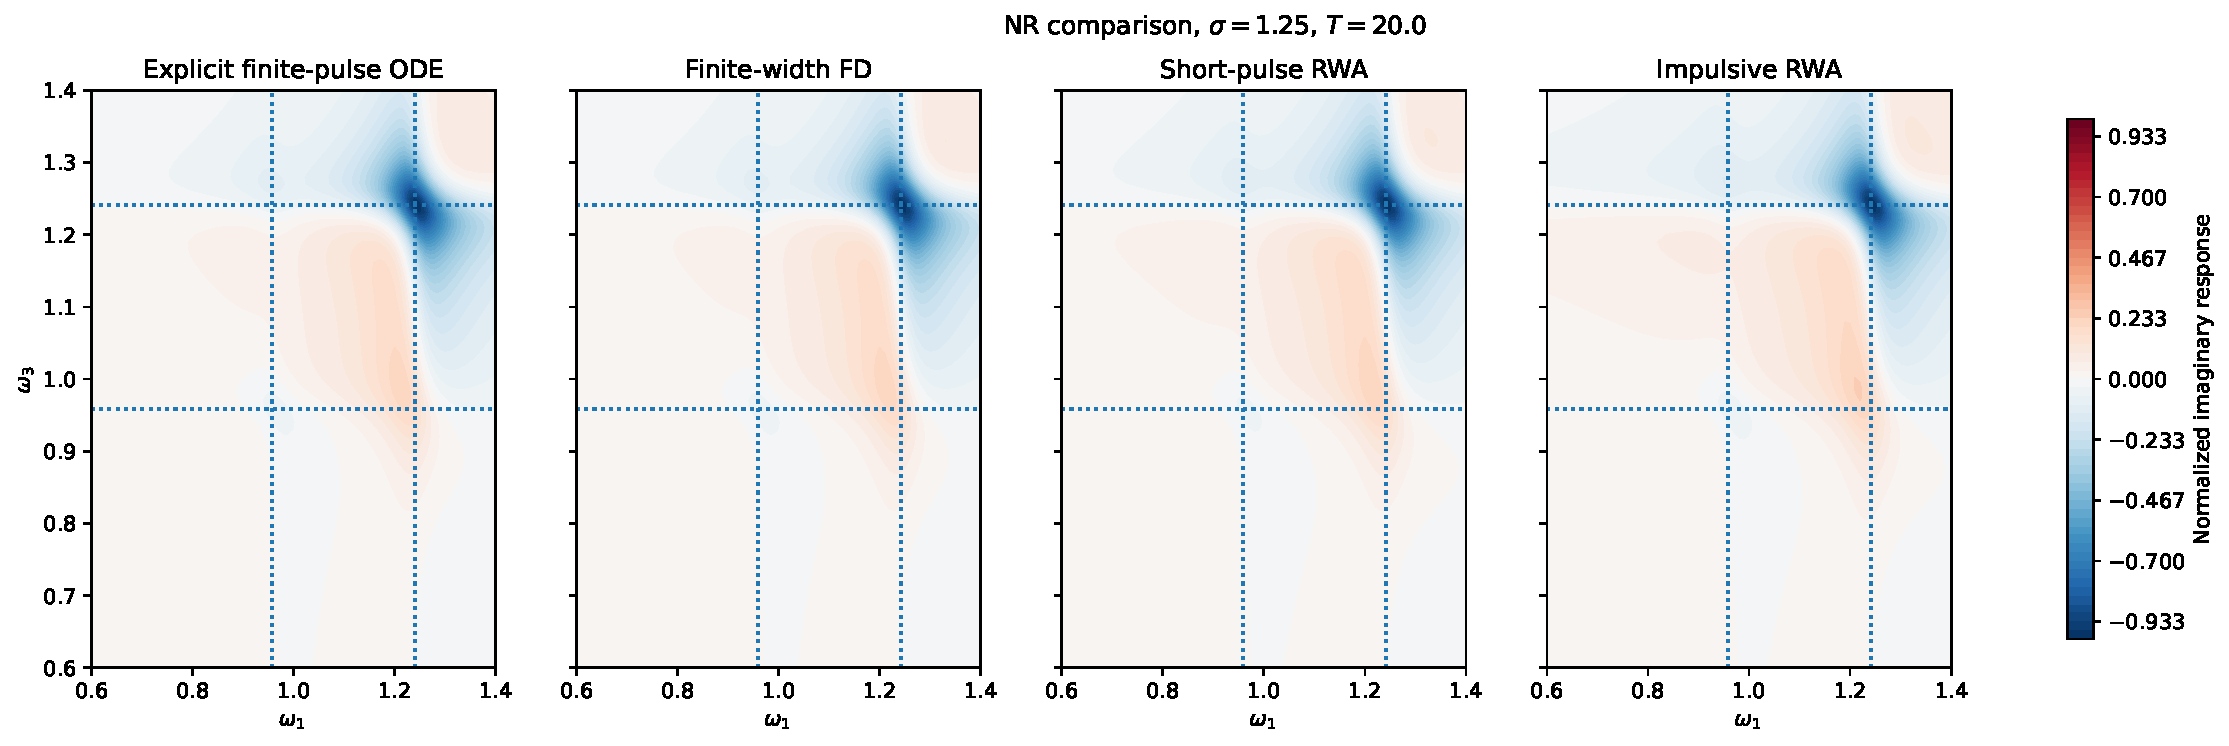
\includegraphics[width=0.98\textwidth]{figures/04_finite_pulse_validation/NR_four_model_sigma1p25_T20_tmax160.pdf}

    \vspace{0.8em}

    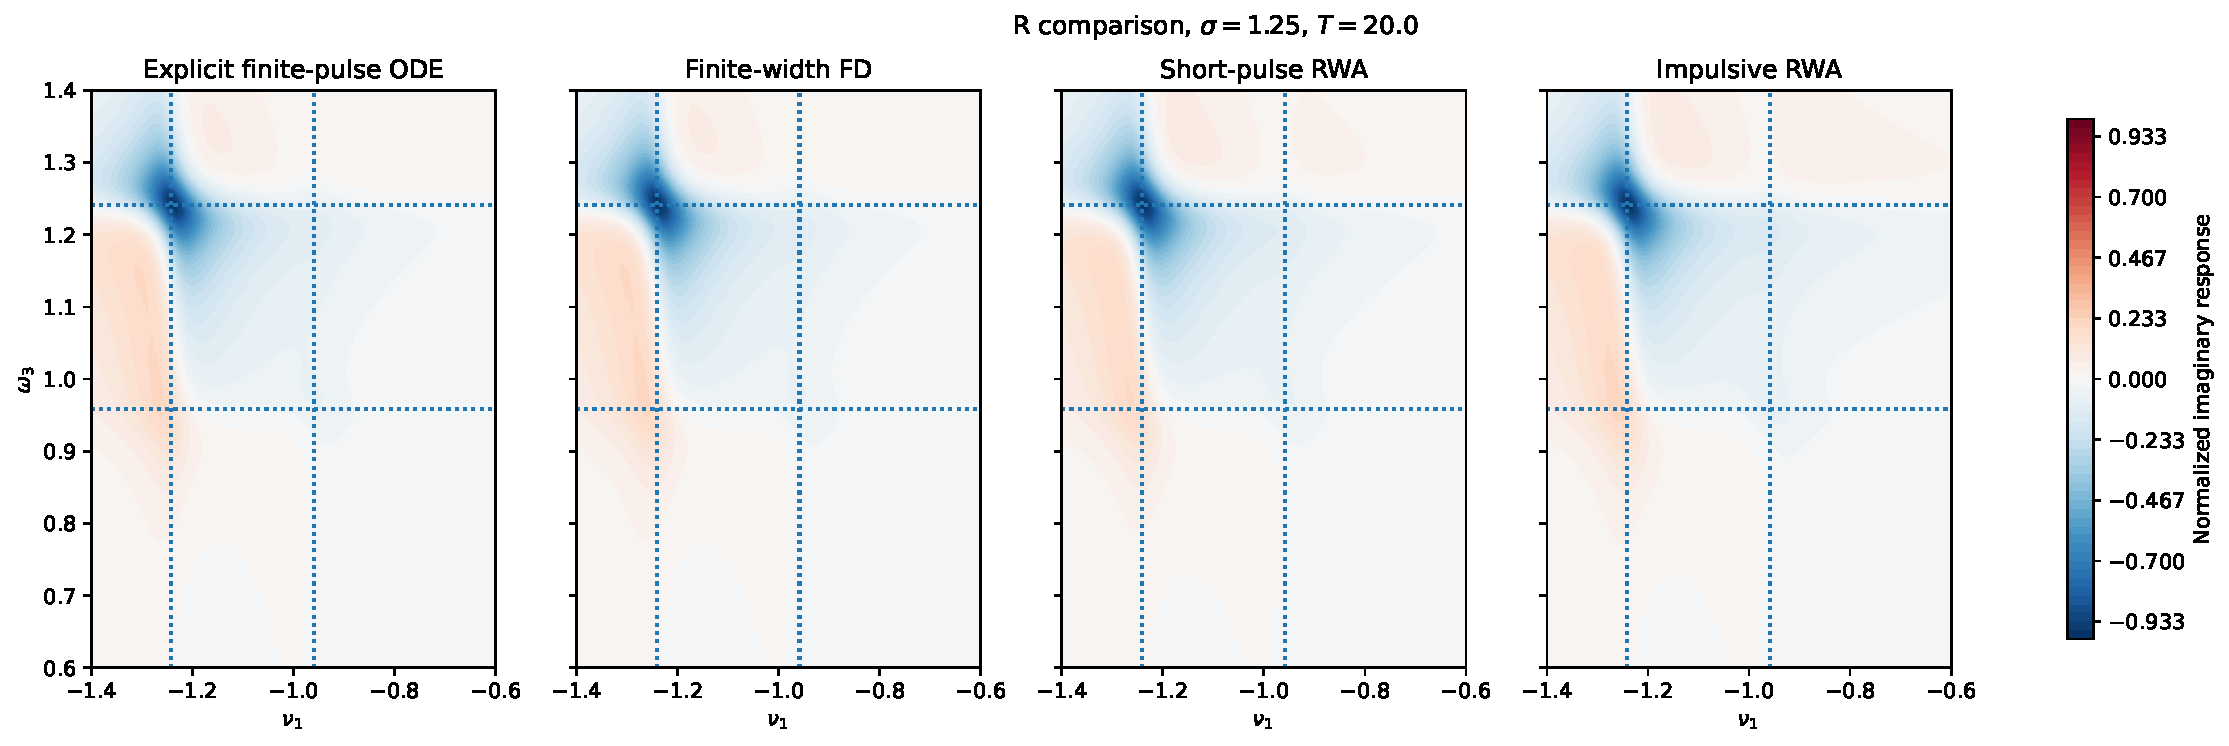
\includegraphics[width=0.98\textwidth]{figures/04_finite_pulse_validation/R_four_model_sigma1p25_T20_tmax160.pdf}

    \caption{
    Comparison of explicit finite-pulse ODE propagation, the
    finite-width direct frequency-domain calculation, the short-pulse
    RWA approximation, and the impulsive RWA response for
    $\sigma=1.25$ and $T=20$.
    The upper panel shows the nonrephasing response and the lower panel
    shows the rephasing response.
    The complete complex spectral-shape discrepancies relative to the
    finite-pulse ODE are approximately $0.059\%$ for the finite-width
    frequency-domain calculation, $5.3$--$5.5\%$ for the short-pulse
    RWA description, and $9.6$--$9.8\%$ for the impulsive RWA response.
    }

    \label{fig:third_order_four_model_finite_width}
\end{figure}

The sub-$0.1\%$ agreement of the converged finite-width calculation
with explicit finite-pulse propagation provides the principal
numerical validation of the operator-valued pulse construction.


% ============================================================
\subsubsection{Pulse-width regimes}
% ============================================================

The Gaussian pulse width was next varied while the waiting time was
held fixed at

\begin{equation}
T=20.
\end{equation}

Only pulse widths for which neighboring pulses remain well separated
are included in the present comparison.  The scan reveals three
distinct physical regimes.

For very short pulses, the optical bandwidth becomes sufficiently broad
that counter-rotating contributions contained in the complete
interaction superoperator are no longer strongly suppressed.  In this
regime the short-pulse RWA and impulsive RWA calculations approach one
another, because molecular evolution during the narrow pulse is
negligible, but both differ appreciably from the full-$V$ result.

At

\begin{equation}
\sigma=0.05,
\end{equation}

for example, the short-pulse and impulsive RWA discrepancies are both

\begin{equation}
\epsilon_{\mathrm{shape}}
\simeq
13.27\%,
\end{equation}

whereas the finite-width frequency-domain result remains within
approximately $0.40\%$ of the full-$V$ ODE reference.

This behavior demonstrates that the limit $\sigma\rightarrow0$ should
not be identified automatically with the conventional impulsive RWA
limit.  The full-$V$ finite-pulse response approaches the impulsive
full-interaction response, whereas the short-pulse RWA expression
approaches the impulsive RWA response.

At intermediate pulse widths, the pulse becomes sufficiently long on
the optical timescale to suppress rapidly oscillating
counter-rotating contributions while remaining short compared with the
slower molecular dynamics.  This produces the conventional
impulsive-RWA window.

For the present dimer, the short-pulse RWA discrepancy reaches its
minimum near

\begin{equation}
\sigma
\simeq
1\text{--}2,
\end{equation}

where it is approximately $5.3\%$.

This intermediate region is the regime in which conventional
impulsive RWA pathway methods, including the QuDPy calculation
validated in Sec.~\ref{subsec:third_order_impulsive}, are physically
most appropriate.  The QuDPy benchmark and the present pulse-width scan
use different numerical preparations and should therefore be regarded
as complementary validations rather than as point-by-point identical
calculations.

As the pulse width increases further, evolution of the molecular state
during the pulse becomes increasingly important.  The impulsive
approximation then deteriorates even when the RWA remains qualitatively
reasonable.

At

\begin{equation}
\sigma=4,
\end{equation}

the impulsive RWA discrepancy has increased to approximately

\begin{equation}
29.4\%,
\end{equation}

while the short-pulse RWA discrepancy is approximately

\begin{equation}
9.0\%.
\end{equation}

The finite-width frequency-domain result remains near

\begin{equation}
0.43\%.
\end{equation}

The approximately $0.4\%$ finite-width floor in this pulse-width scan
is caused primarily by the shorter numerical Fourier window
$t_{\max}=120$ used for the scan.  As shown above, increasing the
window to $t_{\max}=160$ reduces the discrepancy near
$\sigma=1.25$ to approximately $0.06\%$.

The three pulse-width regimes are summarized in
Fig.~\ref{fig:third_order_three_regimes}.

\begin{figure}[htbp]
    \centering

    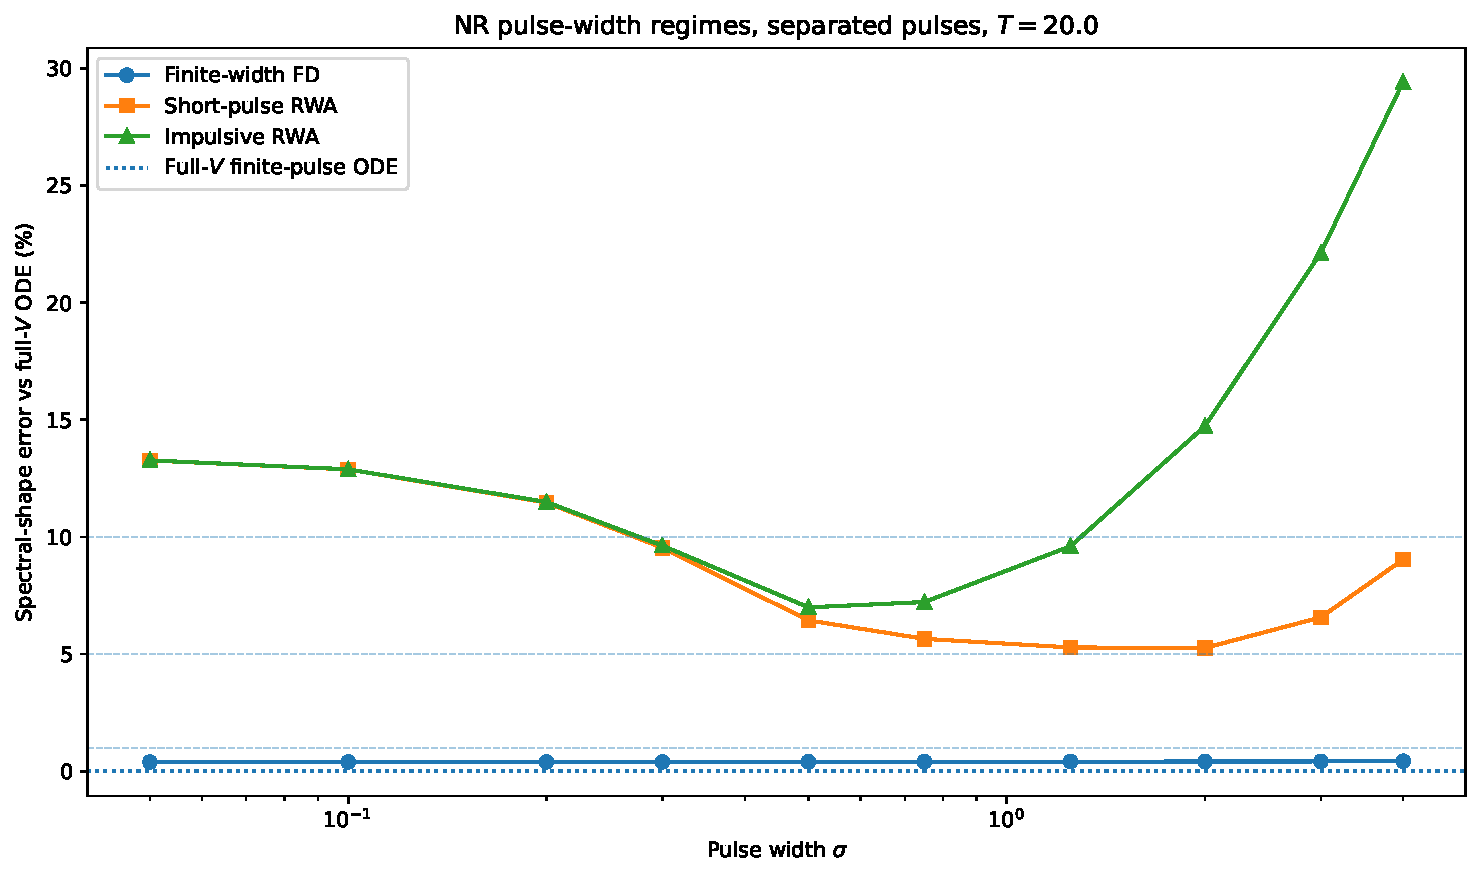
\includegraphics[width=0.82\textwidth]{figures/04_finite_pulse_validation/NR_three_physical_regimes.pdf}

    \caption{
    Spectral-shape discrepancy of the finite-width frequency-domain,
    short-pulse RWA, and impulsive RWA calculations relative to the
    full-$V$ finite-pulse ODE as a function of Gaussian pulse width.
    The scan is restricted to the separated-pulse domain.
    The ultrashort region displays non-RWA corrections, the
    intermediate region provides the conventional impulsive-RWA
    window, and finite-pulse dynamical effects become progressively
    more important as the pulse width increases.
    The approximately $0.4\%$ floor of the finite-width curve is
    associated with the finite Fourier window used for this scan.
    }

    \label{fig:third_order_three_regimes}
\end{figure}


% ============================================================
\subsubsection{Validity of the separated-pulse approximation}
% ============================================================

The factorized finite-width expression in
Eq.~\eqref{eq:third_order_finite_validation} assumes that the three
pulse envelopes are temporally separated.  It is therefore important
to distinguish the finite-pulse regime from the separate breakdown
caused by direct pulse overlap.

For two equal Gaussian envelopes separated by a time
$\Delta\tau$,

\begin{equation}
g_1(t)
=
\exp\left[
-\frac{(t-\tau_1)^2}{2\sigma^2}
\right],
\end{equation}

and

\begin{equation}
g_2(t)
=
\exp\left[
-\frac{(t-\tau_2)^2}{2\sigma^2}
\right],
\end{equation}

the normalized envelope overlap is

\begin{equation}
\mathcal{O}
=
\frac{
\int dt\,
g_1(t)g_2(t)
}{
\sqrt{
\int dt\,g_1^2(t)
\int dt\,g_2^2(t)
}
}
=
\exp\left[
-\frac{\Delta\tau^2}{4\sigma^2}
\right].
\label{eq:third_order_gaussian_overlap}
\end{equation}

If an overlap tolerance $\varepsilon$ is required, then

\begin{equation}
\frac{\Delta\tau}{\sigma}
>
2
\sqrt{
\ln\left(
\frac{1}{\varepsilon}
\right)
}.
\label{eq:third_order_gaussian_separation}
\end{equation}

For example,

\begin{equation}
\mathcal{O}<1\%
\end{equation}

requires approximately

\begin{equation}
\frac{\Delta\tau}{\sigma}
>
4.29,
\end{equation}

whereas

\begin{equation}
\mathcal{O}<0.1\%
\end{equation}

requires approximately

\begin{equation}
\frac{\Delta\tau}{\sigma}
>
5.26.
\end{equation}

The sequential ODE of
Eq.~\eqref{eq:third_order_finite_ode} imposes the chronological pulse
ordering $1\rightarrow2\rightarrow3$. To verify that this restriction
does not affect the separated-pulse benchmark, we performed a second,
unrestricted propagation under the complete time-dependent
three-pulse field. In this calculation, all three finite pulses are
present simultaneously, the complete interaction superoperator $V$ is
retained, and no chronological ordering of the individual
light--matter interactions is imposed.

The desired rephasing or nonrephasing contribution is isolated by
numerical phase cycling. Four equally spaced carrier phases are used
for each of the three pulses, producing

\begin{equation}
4^3=64
\end{equation}

full-field propagations. The selected third-order field signature is
then obtained by discrete Fourier projection with respect to the three
carrier phases, as described in
Appendix~\ref{app:phase_resolved_propagation}.

Because the complete driven propagation contains all orders of the
field, the phase-cycle benchmark is performed in the weak-field regime
so that the selected phase component is dominated by the desired
third-order response. The phase-projection procedure was independently
validated against the perturbative third-order response, with relative
discrepancies of order $6\times10^{-5}$ for both the rephasing and
nonrephasing branches.

For $\sigma=1.25$, inclusion of the region near zero pulse-1/pulse-2
separation produces a spectral-shape difference of approximately

\begin{equation}
7.70\%
\end{equation}

between the unrestricted three-pulse calculation and the sequential
ODE.

The discrepancy falls rapidly as the minimum pulse separation is
increased.  At a separation of approximately

\begin{equation}
4\sigma,
\end{equation}

the spectral-shape difference is only approximately

\begin{equation}
0.025\%,
\end{equation}

and by approximately $5$--$6\sigma$ it falls below

\begin{equation}
10^{-3}\%.
\end{equation}

This explicitly verifies that the sequential full-$V$ ODE becomes
equivalent to the unrestricted three-pulse propagation in the regime
where neighboring Gaussian pulse overlaps are negligible.

The connection between envelope overlap and temporal-ordering
corrections is shown in
Fig.~\ref{fig:third_order_ordering_overlap}.

\begin{figure}[htbp]
    \centering

    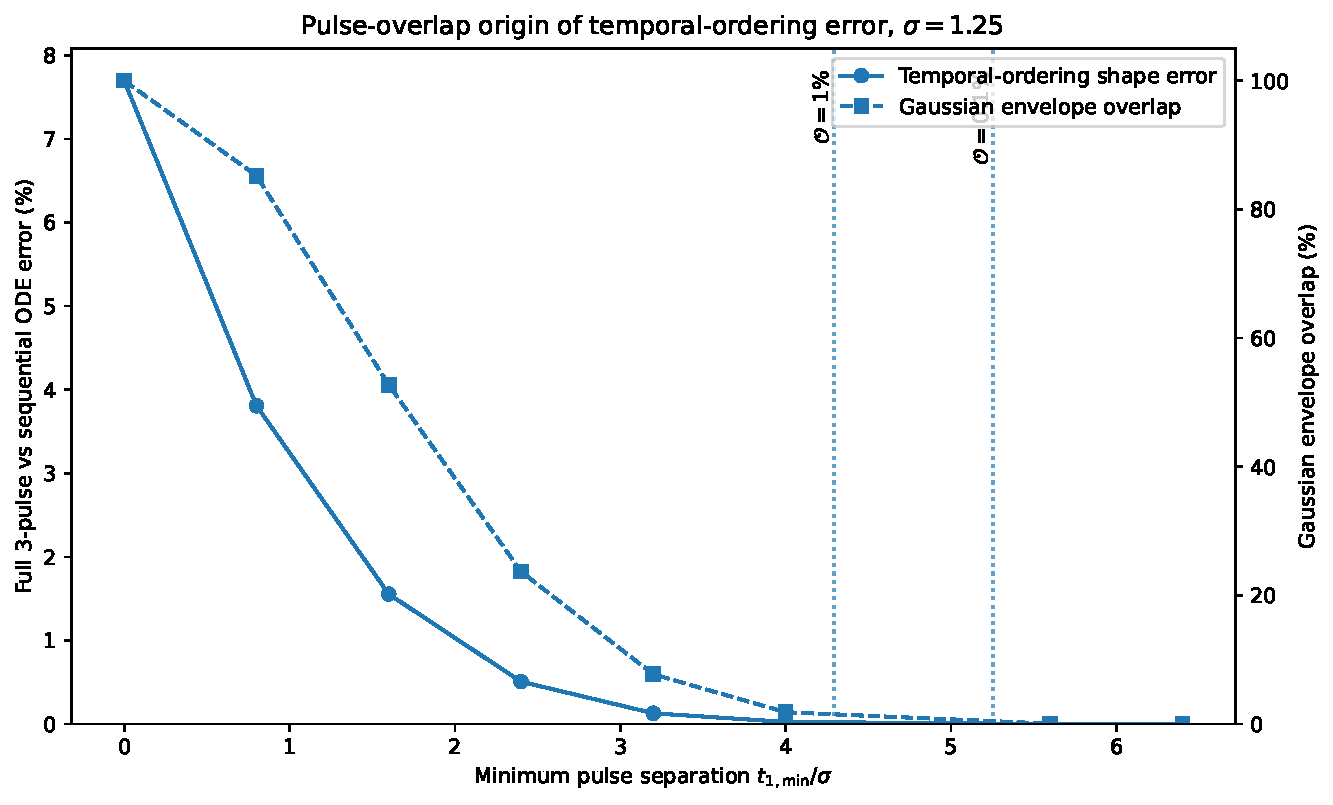
\includegraphics[width=0.78\textwidth]{figures/04_finite_pulse_validation/NR_ordering_error_and_overlap_dual_axis.pdf}

    \caption{
    Comparison of Gaussian pulse overlap with the spectral-shape
    difference between the unrestricted three-pulse ODE and the
    sequential full-$V$ third-order ODE.
    The nonrephasing calculation is shown for $\sigma=1.25$ while
    progressively excluding small pulse-1/pulse-2 separations.
    Temporal-ordering corrections decrease rapidly with the Gaussian
    overlap and become negligible once neighboring pulses are separated
    by approximately $4$--$5\sigma$.
    }

    \label{fig:third_order_ordering_overlap}
\end{figure}

The finite-width frequency-domain formulation therefore has a clear
domain of validity.  Within the separated-pulse regime it reproduces
explicit full-$V$ finite-pulse propagation with sub-percent numerical
error and remains accurate across the ultrashort, conventional
impulsive-RWA, and finite-pulse regimes.  When neighboring pulse
envelopes overlap strongly, additional temporal orderings contribute
and the separated-pulse factorization is no longer expected to apply.

% ============================================================
\subsection{Summary of the Numerical Validation}
\label{subsec:numerical_validation_summary}
% ============================================================

The calculations in this section establish a sequence of independent
numerical checks of the direct frequency-domain formulation, beginning
with linear response and extending to finite-pulse third-order
spectroscopy.

At linear order, direct Lindblad propagation and Liouville-space
propagation agree to numerical precision.  Explicit time-domain
propagation followed by Fourier transformation reproduces the direct
Liouvillian-resolvent response, and for a stationary preparation the
finite-pulse polarization factorizes as

\begin{equation}
P^{(1)}(\omega)
=
E(\omega)
M^{(1)}(\omega).
\end{equation}

The nonstationary prepared-state calculation further demonstrates that
deviations from this simple factorization can be attributed to
field-free evolution of the preparation rather than to a failure of
the resolvent construction.

At third order, the impulsive response calculated from explicit
two-dimensional time-domain propagation agrees with the direct
frequency-domain resolvent expression with a relative complex
discrepancy of approximately

\begin{equation}
5.4\times10^{-5}.
\end{equation}

This comparison uses the complete interaction superoperator $V$ and
therefore validates the direct frequency-domain construction
independently of the rotating-wave approximation.

The subsequent RWA-resolved rephasing and nonrephasing calculations
were independently compared with QuDPy time-domain pathway
propagation.  The complete complex two-dimensional spectra agree at the
approximately

\begin{equation}
1.4\%
\end{equation}

level without amplitude normalization or phase correction.  This
provides an independent check of the excitation-raising and
excitation-lowering interaction decomposition, the pathway signs, and
the rephasing/nonrephasing conventions.

The finite-width pulse operators $F_1$, $F_2$, and $F_3$ were tested
directly against their defining Gaussian time integrals and agree to
approximately

\begin{equation}
10^{-13}.
\end{equation}

For the stationary state, the expected identity

\begin{equation}
F_1^{(s_1)}
|\rho_{\mathrm{ss}}\rangle\rangle
=
E_1^{(s_1)}
|\rho_{\mathrm{ss}}\rangle\rangle
\end{equation}

is satisfied to numerical precision.

Most importantly, the complete finite-width frequency-domain
third-order response was compared with explicit finite-pulse
full-$V$ ODE propagation.  For
$\sigma=1.25$ and $T=20$, convergence of the time-domain Fourier
window gives

\begin{equation}
\epsilon_{\mathrm{FD/ODE}}^{NR}
=
0.0586\%,
\end{equation}

and

\begin{equation}
\epsilon_{\mathrm{FD/ODE}}^{R}
=
0.0582\%.
\end{equation}

The corresponding optimal global complex factors are essentially
unity, showing that the agreement is quantitative in both amplitude
and phase and is not produced by an arbitrary rescaling.

The pulse-width scan further separates three physically distinct
regimes.  For ultrashort pulses, the short-pulse and impulsive RWA
responses converge toward one another while remaining different from
the complete full-$V$ response because counter-rotating contributions
are no longer negligible.  At intermediate pulse widths, the
conventional impulsive-RWA description becomes most accurate.  At
larger pulse widths, molecular evolution during the pulse becomes
important and the impulsive approximation progressively fails, while
the finite-width frequency-domain construction continues to reproduce
the explicit finite-pulse ODE.

Finally, comparison with an unrestricted three-pulse ODE establishes
the domain of validity of the separated-pulse factorization.  For equal
Gaussian envelopes, the normalized overlap

\begin{equation}
\mathcal{O}
=
\exp\left[
-\frac{\Delta\tau^2}{4\sigma^2}
\right]
\end{equation}

provides a direct measure of pulse separation.  Temporal-ordering
corrections become negligible once neighboring pulses are separated by
approximately $4$--$5\sigma$, whereas strong pulse overlap introduces
additional chronological orderings that are not contained in the
factorized finite-width expression.

The numerical validation may therefore be summarized schematically as

\begin{equation}
\boxed{
\begin{gathered}
\text{Liouville-space dynamics}
\\
\Downarrow
\\
\text{direct resolvent response}
\\
\Downarrow
\\
\text{impulsive third-order response}
\\
\Downarrow
\\
\text{RWA-resolved rephasing/nonrephasing response}
\\
\Downarrow
\\
\text{finite-width }F_1F_2F_3\text{ response}
\\
\Downarrow
\\
\text{explicit finite-pulse full-}V\text{ ODE}.
\end{gathered}
}
\label{eq:numerical_validation_chain}
\end{equation}

Together, these results validate the direct frequency-domain method in
the impulsive, short-pulse, and finite-width separated-pulse regimes,
while also identifying the physical limits of the simpler RWA and
impulsive approximations and the breakdown of the separated-pulse
factorization under strong temporal overlap.

Having established this numerical foundation, we next turn to a more
systematic comparison of the frequency-domain and time-domain
approaches and to the computational consequences of the different
pulse treatments.

% ============================================================
\section{Computational Performance}
\label{sec:computational_performance}
% ============================================================

The numerical validations in Sec.~\ref{sec:numerical_validation}
establish the equivalence of the direct frequency-domain formulation
with explicit time-domain propagation when the corresponding physical
approximations and transform conventions are matched.  We now examine
the computational cost of the different formulations.

All timing comparisons reported in this section were performed in the
same software environment and on the same machine.  Wall-clock times
were measured repeatedly after warm-up evaluations, and the median
runtime was used to reduce the influence of transient system-level
fluctuations.

We first compare direct resolvent evaluation with explicit
time-domain propagation followed by a two-dimensional Fourier
transform.  We then quantify the additional cost of the finite-pulse
operators, examine the dependence on the requested frequency-grid
density, and analyze the cost required to converge the time-domain
calculation with respect to the coherence-time window and temporal
spacing.  Finally, an implementation-level timing comparison with
QuDPy is presented separately.


% ============================================================
\subsection{Frequency-Domain versus Time-Domain Evaluation}
\label{subsec:fd_vs_td_performance}
% ============================================================

We begin with the impulsive nonrephasing RWA response used in the
validation of Sec.~\ref{subsec:third_order_impulsive}.  The direct
frequency-domain calculation evaluates

\begin{equation}
M_{NR}^{(3)}
(\omega_3,T,\omega_1)
=
\langle\!\langle\mu|
G_\eta(\omega_3)
V_{\uparrow}
e^{\mathcal{L}T}
V_{\downarrow}
G_\eta(\omega_1)
V_{\uparrow}
|\rho_0\rangle\!\rangle ,
\end{equation}

directly on the requested frequency grid.  The corresponding
time-domain calculation first constructs

\begin{equation}
R_{NR}^{(3)}(t_3,T,t_1)
\end{equation}

on a two-dimensional coherence-time grid and subsequently performs the
damped transform

\begin{equation}
M_{NR,\mathrm{TD}}^{(3)}
(\omega_3,T,\omega_1)
=
\int_0^\infty dt_3
\int_0^\infty dt_1\,
e^{(i\omega_3-\eta)t_3}
e^{(i\omega_1-\eta)t_1}
R_{NR}^{(3)}(t_3,T,t_1).
\end{equation}

For the benchmark, the waiting time and damping parameter were

\begin{equation}
T=5,
\qquad
\eta=0.02,
\end{equation}

and the coherence-time axes extended to

\begin{equation}
t_{\max}=100
\end{equation}

with temporal spacing

\begin{equation}
\Delta t=0.25.
\end{equation}

The final spectrum was evaluated on an
$81\times81$ frequency grid over the interval used in the numerical
validation.

The direct frequency-domain calculation required a median wall-clock
time of

\begin{equation}
\boxed{
t_{\mathrm{FD}}
=
1.298\times10^{-3}\ \mathrm{s}.
}
\end{equation}

For the time-domain calculation, explicit propagation required

\begin{equation}
t_{\mathrm{prop}}
=
3.726\times10^{-3}\ \mathrm{s},
\end{equation}

while the subsequent two-dimensional transform required

\begin{equation}
t_{\mathrm{FT}}
=
0.934\times10^{-3}\ \mathrm{s}.
\end{equation}

The total time-domain cost was therefore

\begin{equation}
\boxed{
t_{\mathrm{TD}}
=
t_{\mathrm{prop}}
+
t_{\mathrm{FT}}
=
4.660\times10^{-3}\ \mathrm{s}.
}
\end{equation}

For this benchmark,

\begin{equation}
\boxed{
\frac{t_{\mathrm{TD}}}{t_{\mathrm{FD}}}
=
3.59.
}
\end{equation}

Thus, for the same physical nonrephasing response and the same
$81\times81$ requested output grid, the direct resolvent evaluation is
approximately $3.6$ times faster than the present time-domain
calculation followed by transformation.

This comparison is not yet accuracy matched: at
$t_{\max}=100$ and $\Delta t=0.25$, the transformed time-domain
spectrum still differs from the direct resolvent by approximately
$1.08\%$. The computational cost required to converge the
time-domain result systematically toward the direct response is
examined separately in Sec.~\ref{subsec:time_window_scaling}.

The dominant contribution to the time-domain runtime is the
construction of the two-dimensional response itself rather than the
Fourier transformation.  Approximately $80\%$ of the total
time-domain wall-clock time is associated with propagation over the
$t_1$ and $t_3$ axes.  The direct frequency-domain formulation avoids
this intermediate coherence-time response and evaluates the requested
spectral points directly.



% ============================================================
\subsection{Cost of Finite-Pulse Dressing}
\label{subsec:finite_pulse_cost}
% ============================================================

We next quantify the additional computational cost associated with
including the temporal and spectral structure of finite laser pulses.
Three frequency-domain formulations are compared on the same
$81\times81$ spectral grid:

\begin{enumerate}
    \item the impulsive RWA response,
    \item the short-pulse RWA response with scalar Gaussian spectral
    factors, and
    \item the finite-width response retaining the operator-valued
    pulse-dressing matrices $F_1$, $F_2$, and $F_3$ together with the
    full interaction superoperator $V$.
\end{enumerate}

The short-pulse formulation retains the spectral envelopes of the
three pulses while neglecting molecular evolution across their
temporal widths.  For the nonrephasing field signature $(+,-,+)$, the
response can therefore be written schematically as

\begin{equation}
P_{\mathrm{short}}^{(3)}
(\omega_3,T,\omega_1)
=
E_3^{(+)}(\omega_3)
E_2^{(-)}(-\omega_1)
E_1^{(+)}(\omega_1)
M_{NR}^{(3)}
(\omega_3,T,\omega_1),
\end{equation}

so that the finite laser pulses enter only through scalar
frequency-dependent factors.

By contrast, the finite-width formulation retains molecular evolution
during the pulse offsets through the operator-valued factors derived
in Sec.~\ref{sec:finite_pulses}. The corresponding response has the
form

\begin{equation}
\begin{aligned}
P_{\mathrm{finite}}^{(3)}
(\omega_3,T,\omega_1)
=
\langle\!\langle\mu|
&G_\eta(\omega_3)
V
e^{\mathcal{L}T}
F_3^{(+)}(\omega_3)
F_2^{(-)}(\omega_1)
V
\\
&\times
G_\eta(\omega_1)
V
F_1^{(+)}(\omega_1)
|\rho_{\mathrm{ss}}\rangle\rangle .
\end{aligned}
\end{equation}

with the appropriate frequency arguments and field-component signs
understood for each $F_j$.

For the benchmark we use Gaussian pulses with

\begin{equation}
\sigma=1.25,
\end{equation}

and evaluate the three formulations on the same frequency grid.  The
median wall-clock time for the impulsive RWA calculation is

\begin{equation}
\boxed{
t_{\mathrm{imp}}
=
1.299\times10^{-3}\ \mathrm{s}.
}
\end{equation}

Including the scalar Gaussian pulse factors increases the runtime only
slightly,

\begin{equation}
\boxed{
t_{\mathrm{short}}
=
1.334\times10^{-3}\ \mathrm{s},
}
\end{equation}

corresponding to

\begin{equation}
\frac{
t_{\mathrm{short}}
}{
t_{\mathrm{imp}}
}
=
1.027.
\end{equation}

Thus, within this implementation, the computational overhead of the
short-pulse scalar dressing is approximately $2.7\%$.

The finite-width calculation requires

\begin{equation}
\boxed{
t_{\mathrm{finite}}
=
7.336\times10^{-3}\ \mathrm{s}.
}
\end{equation}

Relative to the short-pulse formulation,

\begin{equation}
\boxed{
\frac{
t_{\mathrm{finite}}
}{
t_{\mathrm{short}}
}
=
5.50,
}
\end{equation}

while relative to the impulsive calculation,

\begin{equation}
\boxed{
\frac{
t_{\mathrm{finite}}
}{
t_{\mathrm{imp}}
}
=
5.65.
}
\end{equation}

The increased cost arises primarily from the construction and
application of the matrix-valued finite-pulse operators.  Whereas the
short-pulse treatment requires only scalar spectral-envelope
multiplications, the finite-width response evaluates matrix functions
of the Liouvillian for the pulse-dressing factors and applies them
within the third-order response sequence.

This additional cost should be interpreted together with the physical
content of the approximations.  The three calculations are not merely
different numerical implementations of the same response.  The
finite-width formulation retains molecular evolution during the pulse
offsets and the full interaction superoperator, whereas the impulsive
and short-pulse RWA expressions neglect some or all of these effects.
Consequently, the factor of approximately $5.5$ represents the
computational price of the additional finite-pulse dynamics rather
than an inefficiency relative to an equivalent calculation.

For the present $16$-dimensional Liouville-space benchmark, the
complete finite-width $81\times81$ spectrum is nevertheless obtained
in approximately $7.3$ ms.  The results therefore show that
operator-valued pulse dressing introduces a measurable but still
modest absolute computational cost for the present model.

The finite-width runtime should therefore not be compared directly
with the impulsive time-domain runtime of
Sec.~\ref{subsec:fd_vs_td_performance} as though the two calculations
represented identical physical approximations. The present benchmark
quantifies the additional cost within the frequency-domain hierarchy
itself.

% ============================================================
\subsection{Scaling with Requested Frequency-Grid Density}
\label{subsec:frequency_grid_scaling}
% ============================================================

The previous benchmark considered a fixed $81\times81$ spectral grid.
We next examine how the computational cost changes as the number of
requested frequency samples is increased.

We denote by $N_\omega$ the number of requested frequencies along each
spectral axis.  The resulting two-dimensional spectrum therefore
contains

\begin{equation}
\boxed{
N_{\mathrm{spec}}
=
N_\omega^2
}
\end{equation}

complex spectral points.  For example,

\begin{equation}
N_\omega=201
\end{equation}

corresponds to a $201\times201$ spectrum containing

\begin{equation}
40\,401
\end{equation}

spectral points.

Importantly, increasing $N_\omega$ at fixed frequency interval only
increases the density with which the final spectrum is sampled.  It
does not by itself improve the intrinsic Fourier resolution of a
finite-time calculation.  The latter is controlled primarily by the
coherence-time window and is examined separately in
Sec.~\ref{subsec:time_window_scaling}.

For the present benchmark, the frequency interval was held fixed at

\begin{equation}
0.6
\leq
\omega_1,\omega_3
\leq
1.4,
\end{equation}

while $N_\omega$ was varied.  The time-domain calculation retained the
same coherence-time grid,

\begin{equation}
t_{\max}=100,
\qquad
\Delta t=0.25,
\end{equation}

for all values of $N_\omega$.

The two approaches have different computational structures.  In the
time-domain formulation, the molecular response
$R^{(3)}(t_3,T,t_1)$ is propagated once on the fixed time grid.
Increasing $N_\omega$ therefore affects only the cost of transforming
this previously generated response onto a denser frequency grid.  The
total time-domain cost can be written as

\begin{equation}
t_{\mathrm{TD}}(N_\omega)
=
t_{\mathrm{prop}}
+
t_{\mathrm{FT}}(N_\omega),
\end{equation}

where $t_{\mathrm{prop}}$ is independent of the number of requested
frequency points.

The direct frequency-domain formulation instead evaluates the
resolvent response directly at the requested frequencies.  Its cost
therefore increases continuously with $N_\omega$.  The implementation
used here also exploits multiple right-hand sides when applying the
$\omega_3$ resolvent, so that the full $N_\omega^2$ spectrum does not
require $N_\omega^2$ completely independent linear solves.

For sparse and moderately sized frequency grids, the avoidance of the
two-dimensional time-domain propagation provides a substantial
advantage.  At

\begin{equation}
N_\omega=21,
\end{equation}

corresponding to only $441$ spectral points, the measured runtimes are

\begin{equation}
t_{\mathrm{FD}}
=
2.44\times10^{-4}\ \mathrm{s},
\end{equation}

and

\begin{equation}
t_{\mathrm{TD}}
=
4.00\times10^{-3}\ \mathrm{s},
\end{equation}

giving

\begin{equation}
\boxed{
\frac{t_{\mathrm{TD}}}{t_{\mathrm{FD}}}
=
16.4.
}
\end{equation}

For the standard $81\times81$ benchmark, the corresponding ratio is

\begin{equation}
\frac{t_{\mathrm{TD}}}{t_{\mathrm{FD}}}
\simeq
3.6,
\end{equation}

in agreement with the direct timing comparison of
Sec.~\ref{subsec:fd_vs_td_performance}.

As the requested grid becomes increasingly dense, the advantage of
direct frequency-domain evaluation decreases.  At approximately

\begin{equation}
N_\omega=201,
\end{equation}

the two runtimes differ by only about $20\%$.  Extending the scan to
larger grids reveals a crossover between

\begin{equation}
N_\omega=241
\end{equation}

and

\begin{equation}
N_\omega=261.
\end{equation}

The corresponding measured runtime ratios are

\begin{equation}
\frac{t_{\mathrm{TD}}}{t_{\mathrm{FD}}}
=
1.06
\qquad
(N_\omega=241),
\end{equation}

and

\begin{equation}
\frac{t_{\mathrm{TD}}}{t_{\mathrm{FD}}}
=
0.95
\qquad
(N_\omega=261).
\end{equation}

Thus, for the present implementation and model, the crossover occurs
near

\begin{equation}
\boxed{
N_\omega
\sim
250,
}
\end{equation}

corresponding to approximately

\begin{equation}
N_\omega^2
\sim
6.3\times10^4
\end{equation}

requested spectral points.

For still denser uniform grids, the explicit time-domain calculation
becomes faster.  At

\begin{equation}
N_\omega=401,
\end{equation}

the measured ratio is

\begin{equation}
\frac{t_{\mathrm{TD}}}{t_{\mathrm{FD}}}
=
0.55,
\end{equation}

so that the time-domain calculation is approximately $1.8$ times
faster for this dense output grid.

These results identify the computational regime in which direct
frequency-domain evaluation is most advantageous.  The largest gains
occur when only selected frequencies or a moderately sized spectral
window is required.  In this regime, the direct method avoids
constructing a complete two-dimensional coherence-time response that
may contain substantially more intermediate data than are ultimately
needed.

For very dense uniform frequency grids, however, the cost of evaluating
many frequency-dependent resolvents eventually exceeds the fixed
propagation cost of the time-domain calculation followed by
transformation.  The precise crossover depends on the Liouville-space
dimension, linear-algebra implementation, transform algorithm, and
hardware, and should therefore not be regarded as a universal value.

\begin{figure}[htbp]
    \centering

    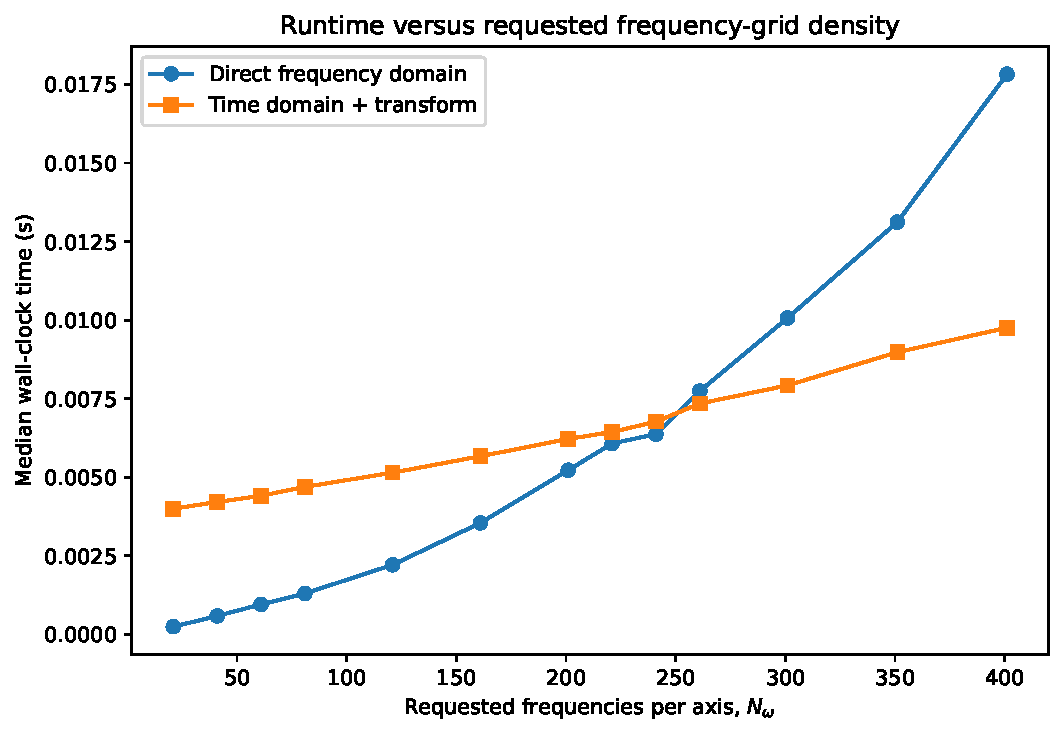
\includegraphics[
        width=0.78\textwidth
    ]{
    figures/05_computational_benchmarks/runtime_vs_frequency_grid_density_final.pdf
    }

    \caption{
    Computational cost as a function of the number of requested
    frequencies per spectral axis, $N_\omega$.  The final
    two-dimensional spectrum contains $N_\omega^2$ spectral points.
    Direct frequency-domain evaluation is substantially faster for
    sparse and moderately sized grids because it avoids construction
    of the intermediate two-dimensional coherence-time response.
    As the requested uniform grid becomes increasingly dense, the
    frequency-dependent resolvent evaluations become progressively
    more expensive and a crossover occurs near $N_\omega\simeq250$
    for the present model and implementation.
    }

    \label{fig:frequency_grid_runtime}
\end{figure}

The comparison also emphasizes that frequency-grid density and
spectral resolution are distinct quantities.  A dense set of
frequency samples can be generated from a fixed finite time window
without increasing the intrinsic frequency resolution.  The
computational consequences of improving the actual finite-time
convergence are considered next.

% ============================================================
\subsection{Time-Window and Temporal-Discretization Convergence}
\label{subsec:time_window_scaling}
% ============================================================

The frequency-grid benchmark of
Sec.~\ref{subsec:frequency_grid_scaling} varies the number of spectral
points requested from a fixed time-domain response.  Increasing
$N_\omega$ therefore increases the sampling density of the final
spectrum but does not improve the convergence associated with the
finite coherence-time window.

A separate question is how the computational cost changes when the
time-domain calculation itself is systematically converged toward the
direct resolvent result.  We examine this dependence first with respect
to the maximum coherence time $t_{\max}$ and subsequently with respect
to the temporal spacing $\Delta t$.

% ------------------------------------------------------------
\subsubsection{Convergence with the coherence-time window}
\label{subsubsec:tmax_convergence}
% ------------------------------------------------------------

For a time-domain Fourier transform extending from zero to
$t_{\max}$, the nominal frequency scale associated with the finite
window is

\begin{equation}
\Delta\omega_{\mathrm{FT}}
\sim
\frac{2\pi}{t_{\max}}.
\end{equation}

This quantity should not be interpreted as the physical linewidth of
the spectrum, which is also determined by the dissipative dynamics and
the finite damping parameter $\eta$.  It instead provides a convenient
measure of the Fourier structure accessible within a finite temporal
window.

For fixed temporal spacing $\Delta t$, the number of points along each
coherence-time axis is approximately

\begin{equation}
N_t
=
\frac{t_{\max}}{\Delta t}+1.
\end{equation}

The complete two-dimensional response therefore contains

\begin{equation}
\boxed{
N_t^2
}
\end{equation}

complex time-domain samples.

To isolate this effect, the requested frequency-domain output was held
fixed at

\begin{equation}
N_\omega=81,
\end{equation}

corresponding to an $81\times81$ spectrum with $6561$ spectral points,
while the temporal spacing was fixed at

\begin{equation}
\Delta t=0.25.
\end{equation}

The coherence-time window was then increased from

\begin{equation}
t_{\max}=25
\end{equation}

to

\begin{equation}
t_{\max}=400.
\end{equation}

For the shortest window, $t_{\max}=25$, the transformed time-domain
spectrum differs from the direct resolvent by approximately

\begin{equation}
40.9\%.
\end{equation}

The time-domain calculation is slightly faster than the direct
frequency-domain evaluation in this case,

\begin{equation}
\frac{t_{\mathrm{TD}}}{t_{\mathrm{FD}}}
=
0.78,
\end{equation}

but the resulting spectrum is far from converged.

Increasing the coherence-time window systematically reduces the
finite-time error.  At

\begin{equation}
t_{\max}=100,
\end{equation}

the relative discrepancy falls to approximately

\begin{equation}
1.08\%,
\end{equation}

while the time-domain calculation becomes

\begin{equation}
\frac{t_{\mathrm{TD}}}{t_{\mathrm{FD}}}
=
3.79
\end{equation}

times slower than the direct resolvent.

At

\begin{equation}
t_{\max}=150,
\end{equation}

the discrepancy is reduced below $0.1\%$,

\begin{equation}
\epsilon_{\mathrm{TD/FD}}
\simeq
0.098\%,
\end{equation}

at a time-domain cost approximately

\begin{equation}
7.46
\end{equation}

times that of the direct frequency-domain calculation.

For

\begin{equation}
t_{\max}=200,
\end{equation}

the discrepancy reaches approximately

\begin{equation}
\boxed{
0.030\%,
}
\end{equation}

while the time-domain runtime is approximately

\begin{equation}
\boxed{
11.7
}
\end{equation}

times the direct frequency-domain runtime.

Further increasing the propagation window to $t_{\max}=300$ and
$t_{\max}=400$ produces little additional improvement in the spectral
agreement.  The relative discrepancy saturates near

\begin{equation}
0.029\%.
\end{equation}

The computational cost nevertheless continues to increase.  At
$t_{\max}=400$,

\begin{equation}
N_t=1601,
\end{equation}

so that the intermediate time-domain response contains

\begin{equation}
\boxed{
1601^2
=
2\,563\,201
}
\end{equation}

complex samples.  The corresponding time-domain calculation is
approximately

\begin{equation}
\boxed{
39.7
}
\end{equation}

times slower than the direct resolvent evaluation of the same final
$81\times81$ spectrum.

The saturation of the error beyond $t_{\max}\approx200$ indicates that
finite-window truncation is no longer the dominant numerical
limitation.  The remaining discrepancy instead reflects the finite
temporal discretization used in the numerical transform.

\begin{figure}[htbp]
    \centering

    \begin{subfigure}[t]{0.48\textwidth}
        \centering

        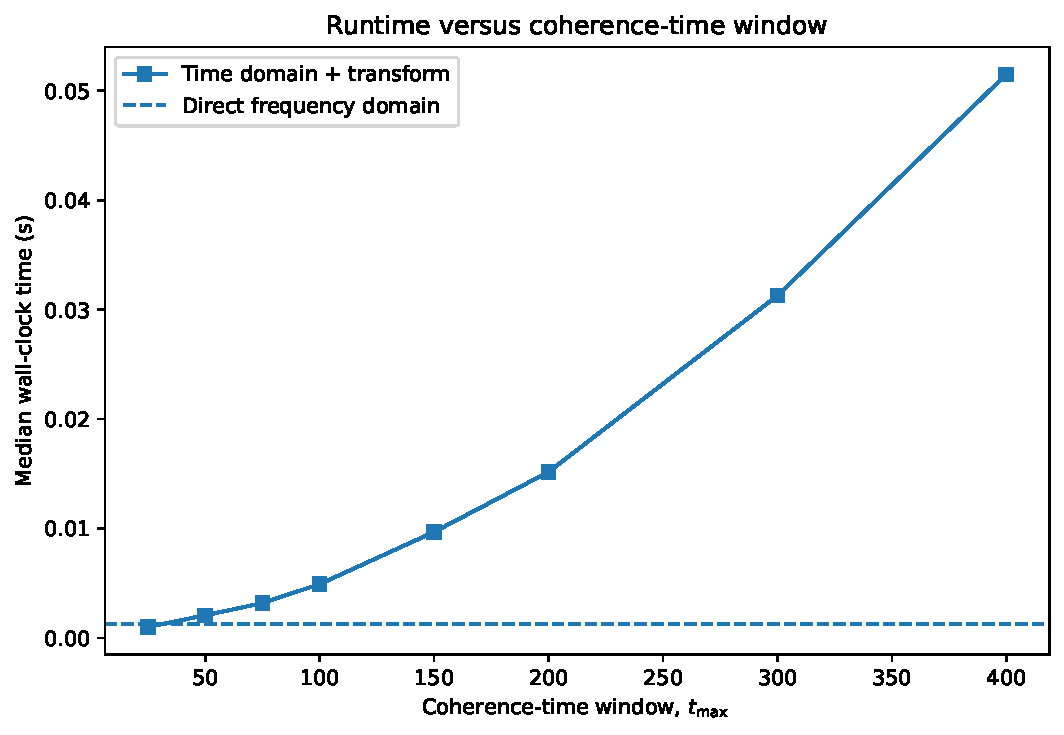
\includegraphics[width=\linewidth]{figures/05_computational_benchmarks/runtime_vs_time_window.pdf}

        \caption{
        Wall-clock time as the coherence-time window is extended.
        The requested frequency-domain output remains fixed at
        $81\times81$ points.
        }

        \label{fig:runtime_vs_time_window}
    \end{subfigure}
    \hfill
    \begin{subfigure}[t]{0.48\textwidth}
        \centering

        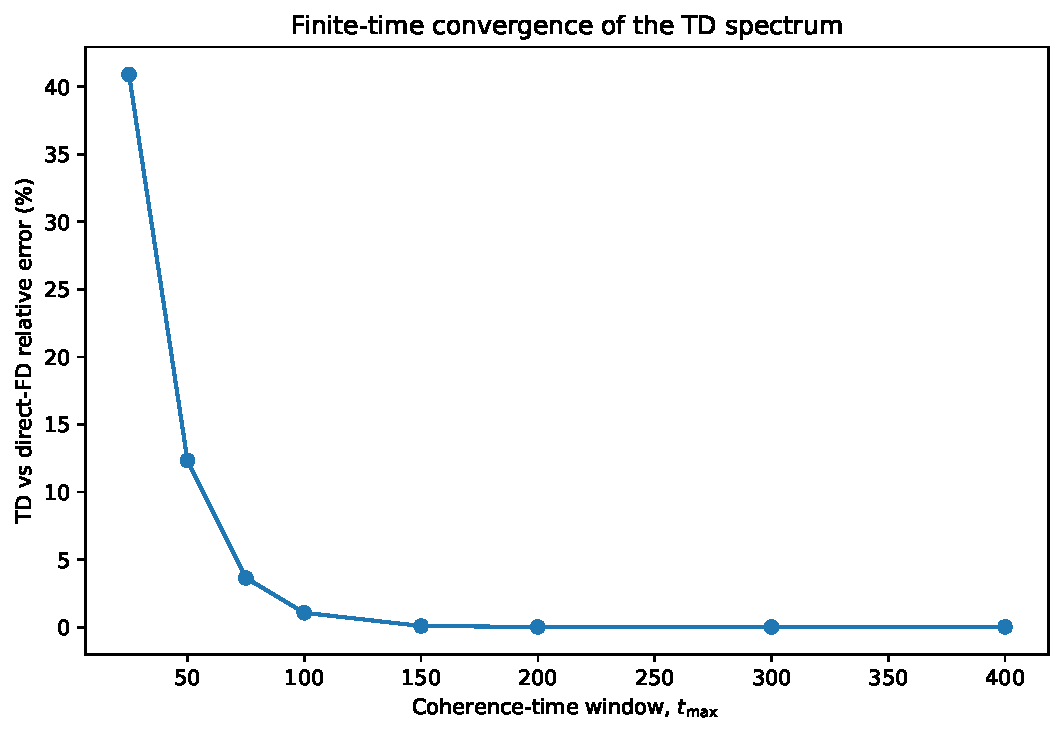
\includegraphics[width=\linewidth]{figures/05_computational_benchmarks/TD_error_vs_time_window.pdf}

        \caption{
        Relative discrepancy between the transformed time-domain
        spectrum and the direct resolvent as $t_{\max}$ is increased.
        }

        \label{fig:error_vs_time_window}
    \end{subfigure}

    \caption{
    Accuracy--cost tradeoff associated with the finite
    coherence-time window.  Increasing $t_{\max}$ systematically
    converges the transformed time-domain response toward the direct
    frequency-domain result, but requires propagation of an
    increasingly large $t_1\times t_3$ response.  The error eventually
    saturates near $0.03\%$ at fixed $\Delta t=0.25$, indicating the
    onset of temporal-discretization error.
    }

    \label{fig:time_window_convergence}
\end{figure}

% ------------------------------------------------------------
\subsubsection{Convergence with temporal discretization}
\label{subsubsec:dt_convergence}
% ------------------------------------------------------------

To verify the origin of the residual error, the coherence-time window
was fixed at

\begin{equation}
t_{\max}=200,
\end{equation}

where finite-window truncation is already small, and the temporal
spacing was successively reduced.

For

\begin{equation}
\Delta t=0.5,
\end{equation}

the relative difference between the transformed time-domain result and
the direct resolvent is

\begin{equation}
0.1166\%.
\end{equation}

Reducing the temporal spacing to

\begin{equation}
\Delta t=0.25
\end{equation}

lowers the discrepancy to

\begin{equation}
0.0302\%.
\end{equation}

A further refinement to

\begin{equation}
\Delta t=0.125
\end{equation}

reduces the error to

\begin{equation}
0.0110\%,
\end{equation}

and at

\begin{equation}
\Delta t=0.0625
\end{equation}

the discrepancy reaches

\begin{equation}
\boxed{
0.0084\%.
}
\end{equation}

The initial reduction from $0.1166\%$ to $0.0302\%$ is close to a
factor of four when $\Delta t$ is halved, consistent with the
second-order convergence expected from the trapezoidal quadrature used
in the numerical Fourier transform.  At finer temporal spacing the
convergence becomes slower, indicating that the remaining
finite-window and numerical errors are becoming comparable to the
quadrature error.

The computational consequence of this refinement is substantial.  At
$\Delta t=0.0625$ and $t_{\max}=200$, each coherence-time axis contains

\begin{equation}
N_t=3201
\end{equation}

points, and the intermediate response therefore contains

\begin{equation}
\boxed{
3201^2
=
10\,246\,401
}
\end{equation}

complex time-domain samples.

This large intermediate representation is required even though the
final requested spectrum still contains only

\begin{equation}
81^2
=
6561
\end{equation}

frequency-domain points.

The combined $t_{\max}$ and $\Delta t$ convergence tests therefore
clarify an important distinction between the two approaches.  A dense
uniform frequency grid can eventually favor a time-domain calculation
once the underlying response has already been propagated.  However,
obtaining a well-converged time-domain spectrum requires a sufficiently
long and finely sampled two-dimensional coherence-time response.  The
direct resolvent formulation avoids both the finite coherence-time
cutoff and the associated intermediate $t_1\times t_3$ representation,
evaluating the requested frequency-domain response directly.

% ============================================================
\subsection{Implementation-Level Comparison with QuDPy}
\label{subsec:qudpy_performance}
% ============================================================

As a final computational benchmark, we compare the direct
frequency-domain implementation with the independent pathway-based
time-domain calculation provided by QuDPy.  This comparison is
intended as an implementation-level benchmark rather than as a
universal comparison between frequency-domain and time-domain
spectroscopy algorithms.

The same coupled-dimer Hamiltonian, Lindblad collapse operators,
ground-state preparation, waiting time, coherence-time range, and
frequency-domain transform convention used in the preceding
nonrephasing benchmark were retained.  The local QuDPy source used for
this calculation was adapted for compatibility with QuTiP~5.

For the nonrephasing signal, QuDPy explicitly propagates the three
double-sided pathways

\begin{equation}
R_4,
\qquad
R_5,
\qquad
R_6,
\end{equation}

generated using the UFSS diagram generator.  The complete
nonrephasing response is then reconstructed as

\begin{equation}
R_{NR}^{(3)}
=
i
\left(
R_4-R_5-R_6
\right).
\end{equation}

The resulting time-domain response was transformed using the same
damped causal Fourier convention employed throughout the present
work, rather than using an independent QuDPy transform convention.

Before comparing runtimes, the QuDPy result was checked against the
direct resolvent calculation.  For the $400\times400$ coherence-time
grid with approximately

\begin{equation}
\Delta t
=
0.2506,
\end{equation}

the complete complex spectra agree with a relative Frobenius
difference of

\begin{equation}
\boxed{
\epsilon_{\mathrm{QuDPy/FD}}
=
1.45\%.
}
\end{equation}

After removal of the small optimal global complex factor as a
diagnostic, the remaining spectral-shape discrepancy is

\begin{equation}
\boxed{
\epsilon_{\mathrm{shape}}
=
1.22\%.
}
\end{equation}

These values reproduce the independent QuDPy validation discussed in
Sec.~\ref{subsec:third_order_impulsive}, confirming that the timing
comparison refers to the same physical nonrephasing response.

Using serial QuDPy propagation, the median total runtime for the three
nonrephasing pathways was approximately

\begin{equation}
4.79\ \mathrm{s}.
\end{equation}

QuDPy's parallel propagation option reduces the corresponding median
propagation time to

\begin{equation}
2.243\ \mathrm{s}.
\end{equation}

The subsequent two-dimensional transform requires only approximately

\begin{equation}
1.01\times10^{-3}\ \mathrm{s},
\end{equation}

so that the complete parallel QuDPy calculation requires approximately

\begin{equation}
\boxed{
t_{\mathrm{QuDPy}}
\simeq
2.244\ \mathrm{s}.
}
\end{equation}

For comparison, the direct frequency-domain calculation of the same
$81\times81$ nonrephasing spectrum requires

\begin{equation}
t_{\mathrm{FD}}
=
1.298\times10^{-3}\ \mathrm{s},
\end{equation}

while the custom explicit time-domain implementation developed for the
present benchmark requires

\begin{equation}
t_{\mathrm{TD}}
=
4.660\times10^{-3}\ \mathrm{s}.
\end{equation}

The corresponding implementation-level runtime ratios are therefore

\begin{equation}
\boxed{
\frac{
t_{\mathrm{QuDPy}}
}{
t_{\mathrm{FD}}
}
\approx
1.7\times10^{3},
}
\end{equation}

and

\begin{equation}
\boxed{
\frac{
t_{\mathrm{QuDPy}}
}{
t_{\mathrm{TD}}
}
\approx
4.8\times10^{2}.
}
\end{equation}

\begin{figure}[htbp]
    \centering

    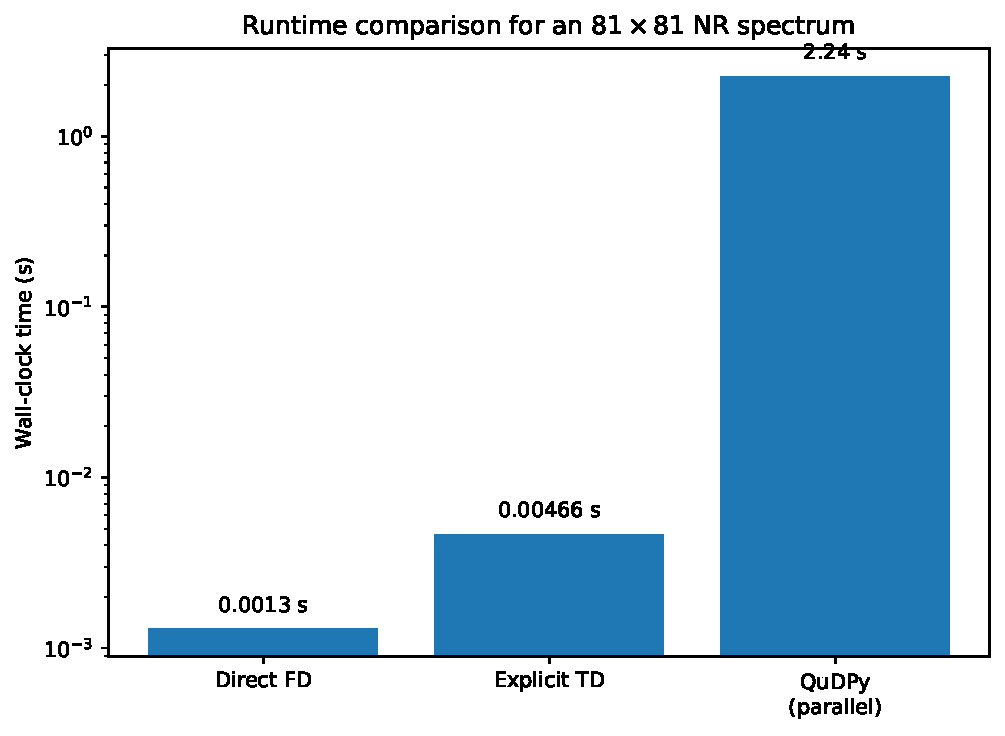
\includegraphics[
        width=0.70\textwidth
    ]{
    figures/05_computational_benchmarks/FD_TD_QuDPy_runtime_comparison.pdf
    }

    \caption{
    Implementation-level wall-clock comparison for the same
    $81\times81$ impulsive nonrephasing RWA spectrum.  Direct
    frequency-domain evaluation is compared with the custom explicit
    time-domain implementation and with parallel QuDPy pathway
    propagation.  A logarithmic vertical scale is used because the
    QuDPy pathway calculation is substantially more expensive for the
    present benchmark.  The QuDPy comparison is implementation
    specific and should not be interpreted as a universal scaling
    relation between frequency-domain and time-domain methods.
    }

    \label{fig:runtime_implementation_comparison}
\end{figure}

The large difference relative to the custom time-domain implementation
arises from the different computational organization of the two
codes.  The present time-domain benchmark propagates the commutator
response directly using matrix operations tailored to the small
Liouville-space model, whereas QuDPy explicitly constructs and
propagates the individual double-sided pathways over the complete
two-dimensional delay grid.

Consequently, the approximately three-orders-of-magnitude difference
between QuDPy and the direct resolvent should not be interpreted as a
general statement that frequency-domain methods are intrinsically
three orders of magnitude faster than all time-domain approaches.
Instead, it demonstrates that, for the present model and software
implementations, direct resolvent evaluation can avoid a substantial
amount of pathway-level time propagation.

The comparison is nevertheless useful because QuDPy provides an
independent and physically validated reference implementation.  The
direct frequency-domain method reproduces the same nonrephasing
spectrum while requiring substantially less wall-clock time for this
benchmark.

% ============================================================
\subsection{Summary of Computational Performance}
\label{subsec:computational_summary}
% ============================================================

The computational benchmarks identify the conditions under which the
direct frequency-domain formulation provides its largest advantage over
explicit time-domain propagation.

For a fixed $81\times81$ impulsive nonrephasing spectrum, direct
resolvent evaluation requires

\begin{equation}
t_{\mathrm{FD}}
=
1.298\times10^{-3}\ \mathrm{s},
\end{equation}

compared with

\begin{equation}
t_{\mathrm{TD}}
=
4.660\times10^{-3}\ \mathrm{s}
\end{equation}

for explicit propagation followed by the two-dimensional transform.
The direct formulation is therefore approximately

\begin{equation}
\boxed{
3.59
}
\end{equation}

times faster for this benchmark.

The advantage is largest when only a limited or moderately sized set
of frequency points is required.  As shown in
Fig.~\ref{fig:frequency_grid_runtime}, the direct method is
approximately $16.4$ times faster for a $21\times21$ output grid.
The advantage decreases as the requested uniform frequency grid
becomes denser, and the two implementations cross near
$N_\omega\sim250$ for the present model.  This crossover reflects the
fact that the time-domain propagation cost is paid only once, whereas
the direct frequency-domain calculation continues to acquire
additional frequency-dependent resolvent cost as $N_\omega$ is
increased.

This dense-grid crossover does not imply that increasing
$N_\omega$ improves the convergence of the underlying time-domain
spectrum.  The number of requested spectral samples and the accuracy
associated with the finite time window are separate numerical
parameters.  Improving the convergence of the explicit time-domain
calculation requires increasing $t_{\max}$ and, eventually, reducing
$\Delta t$.

The convergence benchmarks in
Fig.~\ref{fig:time_window_convergence} show the corresponding
accuracy--cost tradeoff.  At fixed $\Delta t=0.25$, extending the
coherence-time window from $t_{\max}=25$ to $t_{\max}=200$ reduces the
time-domain discrepancy from approximately $40.9\%$ to $0.030\%$.
Over the same range, the time-domain calculation changes from slightly
faster than the direct resolvent to approximately $11.7$ times slower.

Further temporal refinement confirms that the remaining discrepancy is
predominantly numerical rather than physical.  At
$t_{\max}=200$, decreasing the temporal spacing from
$\Delta t=0.5$ to $\Delta t=0.0625$ reduces the relative difference to

\begin{equation}
\boxed{
8.4\times10^{-5},
}
\end{equation}

while increasing the intermediate time-domain response from
$401^2$ to

\begin{equation}
3201^2
=
10\,246\,401
\end{equation}

complex samples.  The final requested frequency-domain spectrum,
however, remains fixed at only

\begin{equation}
81^2
=
6561
\end{equation}

spectral points.

The finite-pulse benchmark shows that the additional physics retained
by the operator-valued pulse dressing also carries a measurable
computational cost.  Scalar short-pulse dressing increases the
impulsive RWA runtime by only approximately $2.7\%$, whereas the full
finite-width calculation is approximately $5.5$ times more expensive
than the short-pulse formulation.  For the present
$16$-dimensional Liouville space, the complete finite-width
$81\times81$ spectrum nevertheless requires only approximately

\begin{equation}
7.3\ \mathrm{ms}.
\end{equation}

Finally, the implementation-level comparison in
Fig.~\ref{fig:runtime_implementation_comparison} shows that the direct
resolvent formulation is substantially faster than the pathway-based
QuDPy implementation for the present benchmark.  Parallel QuDPy
propagation requires approximately $2.24$ s for the same validated
nonrephasing response, compared with $1.30$ ms for the direct
frequency-domain calculation.  This difference is specific to the
software implementations and computational organization considered
here and should not be interpreted as a universal scaling relation
between frequency-domain and time-domain spectroscopy methods.

Taken together, the benchmarks show that the principal computational
advantage of the direct formulation is not simply a uniform reduction
in runtime for every possible spectral calculation.  Its strongest
advantage occurs when selected frequencies, moderately sized spectral
grids, or highly converged frequency-domain responses are required.
In these regimes, the resolvent formulation avoids the construction
and storage of a potentially much larger intermediate
$t_1\times t_3$ response while retaining direct access to the desired
spectral coordinates.


% ============================================================
\section{Limitations and Outlook}
\label{sec:limitations_outlook}
% ============================================================

The numerical results establish the direct frequency-domain
formulation as an accurate and computationally useful alternative to
explicit two-dimensional time-domain propagation within the regime
considered here.  At the same time, the derivation and benchmarks
identify several assumptions that delimit the present scope of the
method.

The most important limitations concern the temporal separation of the
laser pulses, the specification of nonequilibrium preparation
protocols, the scaling of the Liouville-space linear algebra for larger
systems, and the relative efficiency of direct frequency-domain
evaluation for very dense spectral grids.  These limitations do not arise from a single
approximation, but from distinct elements of the present formulation.
They are therefore discussed separately below together with possible
extensions of the method.


% ============================================================
\subsection{Separated-Pulse Approximation}
\label{subsec:separated_pulse_limitation}
% ============================================================

The finite-pulse frequency-domain construction developed in this work
assumes a prescribed chronological ordering of the three laser
interactions.  Molecular evolution during the temporal extent of each
pulse is retained through the operator-valued dressing factors
$F_1$, $F_2$, and $F_3$, but the calculation does not include all
possible temporal interleavings of overlapping pulses.

This distinction is important.  A finite pulse width does not by
itself invalidate the frequency-domain dressing.  The method remains
accurate when molecular evolution during each pulse is significant,
provided that the pulses are sufficiently separated that the sequence
of interactions can still be treated as

\begin{equation}
1
\rightarrow
2
\rightarrow
3.
\end{equation}

To test this assumption independently, the sequential finite-pulse
calculation was compared with an unrestricted phase-resolved
three-pulse propagation that retained the complete time-dependent
field, the full interaction superoperator $V$, and all temporal
orderings. The desired rephasing or nonrephasing field signature was
isolated by phase cycling. Because the unrestricted driven equation
contains all orders of the field, the benchmark was performed in the
weak-field regime in which the selected phase component is dominated
by the third-order response. In the limit of well-separated pulses,
the unrestricted and sequential calculations become numerically
equivalent.

For two Gaussian pulses of equal temporal width $\sigma$ separated by
a delay $\Delta\tau$, a useful measure of their normalized temporal
overlap is

\begin{equation}
\boxed{
\mathcal{O}
=
\exp\left[
-\frac{
\Delta\tau^2
}{
4\sigma^2
}
\right].
}
\label{eq:gaussian_pulse_overlap}
\end{equation}

The overlap decreases rapidly with the dimensionless separation
$\Delta\tau/\sigma$.  For example,

\begin{equation}
\mathcal{O}
\simeq
1.83\times10^{-2}
\qquad
\text{for}
\qquad
\frac{\Delta\tau}{\sigma}=4,
\end{equation}

and

\begin{equation}
\mathcal{O}
\simeq
1.93\times10^{-3}
\qquad
\text{for}
\qquad
\frac{\Delta\tau}{\sigma}=5.
\end{equation}

The unrestricted three-pulse benchmark shows the same trend.
Differences associated with alternative temporal orderings become
small once neighboring pulses are separated by approximately
$4$--$5$ pulse widths.  In this regime, the sequential
frequency-domain construction and the unrestricted time-domain
propagation agree to high numerical accuracy.

As the pulse overlap increases, however, the discrepancy grows because
the unrestricted calculation contains interaction sequences that
cannot be represented by a single prescribed pulse ordering.  The
resulting error is therefore not a failure of the finite-width
operators $F_j$ themselves.  It reflects the breakdown of the
separated-pulse assumption used to organize the perturbative response.

A convenient approximate separation criterion can be obtained from
Eq.~\eqref{eq:gaussian_pulse_overlap}.  Requiring the normalized overlap
to remain below a chosen tolerance $\epsilon_{\mathrm{ov}}$ gives

\begin{equation}
\boxed{
\frac{
\Delta\tau
}{
\sigma
}
>
2
\sqrt{
\ln
\left(
\frac{1}{
\epsilon_{\mathrm{ov}}
}
\right)
}.
}
\label{eq:pulse_overlap_criterion}
\end{equation}

For example, an overlap below $1\%$ requires approximately

\begin{equation}
\frac{
\Delta\tau
}{
\sigma
}
>
4.29,
\end{equation}

consistent with the numerical three-pulse benchmark.

The precise separation required in a particular system will depend on
the pulse envelopes, carrier frequencies, molecular timescales, and
desired numerical accuracy.  The $4$--$5\sigma$ range should therefore
be regarded as a practical result for the present Gaussian benchmark
rather than as a universal boundary.

Extending the direct formulation to strongly overlapping pulses would
require retaining multiple temporal orderings explicitly or developing
a more general multidimensional pulse-dressing construction.  The
phase-resolved three-pulse propagation used here provides a natural
reference for testing such extensions.

% ============================================================
% ============================================================
\subsection{Initial-State Preparation and Time-Translation Invariance}
\label{subsec:initial_state_limitation}
% ============================================================

The finite-pulse formulation is simplest when the state immediately
preceding the pulse sequence is stationary under the field-free
Liouvillian,

\begin{equation}
\mathcal{L}
|\rho_{\mathrm{ss}}\rangle\rangle
=
0.
\end{equation}

In this case, the state is invariant under field-free evolution and
the first finite-width pulse operator reduces exactly to the ordinary
scalar laser spectrum,

\begin{equation}
F_1^{(s_1)}(\omega_1)
|\rho_{\mathrm{ss}}\rangle\rangle
=
E_1^{(s_1)}(\omega_1)
|\rho_{\mathrm{ss}}\rangle\rangle.
\end{equation}

Stationarity is not, however, required by the general finite-width
formulation. If a nonequilibrium state
$|\rho_{\mathrm{prep}}\rangle\rangle$ is prepared at a time
$t_{\mathrm{prep}}$ before the center $\tau_1$ of pulse 1, its
field-free evolution to the pulse center is retained through

\begin{equation}
|\rho_{\mathrm{ref}}\rangle\rangle
=
e^{\mathcal{L}\tau_{\mathrm{prep}}}
|\rho_{\mathrm{prep}}\rangle\rangle,
\qquad
\tau_{\mathrm{prep}}
=
\tau_1-t_{\mathrm{prep}},
\end{equation}

and its additional evolution across the temporal support of pulse 1 is
contained in

\begin{equation}
F_1^{(s_1)}(\omega_1)
|\rho_{\mathrm{ref}}\rangle\rangle.
\end{equation}

Thus, a nonstationary preparation does not require a
frozen-preparation approximation. The complete first-pulse contribution
is

\begin{equation}
\boxed{
F_1^{(s_1)}(\omega_1)
e^{\mathcal{L}\tau_{\mathrm{prep}}}
|\rho_{\mathrm{prep}}\rangle\rangle,
}
\end{equation}

as developed in Sec.~\ref{subsec:dimer_initial_state}.

The linear-response benchmark of
Sec.~\ref{sec:linear_validation} illustrates why this distinction can
matter numerically. To quantify the nonstationarity of the prepared
ground state, we introduced the norm-based drift scale

\begin{equation}
\kappa_0
=
\frac{
\left\|
\mathcal{L}
|\rho_0\rangle\rangle
\right\|_2
}{
\left\|
|\rho_0\rangle\rangle
\right\|_2
}
=
0.0061237.
\end{equation}

Its inverse,

\begin{equation}
\kappa_0^{-1}
\simeq
163.3,
\end{equation}

provides a convenient reference scale but should not be interpreted as
a unique physical relaxation time.

Two useful dimensionless diagnostics are

\begin{equation}
\chi_{\mathrm{width}}
=
\sigma\kappa_0,
\end{equation}

which estimates the magnitude of field-free drift that may accumulate
across the first pulse, and

\begin{equation}
\chi_{\mathrm{delay}}
=
\tau_{\mathrm{prep}}\kappa_0,
\end{equation}

which characterizes the drift accumulated between preparation and the
pulse center.

For the benchmark with

\begin{equation}
\sigma=2,
\qquad
\tau_{\mathrm{prep}}=8,
\end{equation}

these quantities are

\begin{equation}
\chi_{\mathrm{width}}
\simeq
0.0122,
\qquad
\chi_{\mathrm{delay}}
\simeq
0.0490.
\end{equation}

Explicitly retaining the field-free evolution of the prepared state
before and during the pulse produces a response that differs by
approximately $4.5\%$ from a calculation in which the preparation is
artificially frozen. By contrast, the frozen-state propagation agrees
with the corresponding factorized frequency-domain expression to
approximately $0.42\%$. This comparison confirms that the larger
difference originates from the neglected evolution of the
nonstationary preparation rather than from the resolvent construction.

The quantities $\chi_{\mathrm{width}}$ and
$\chi_{\mathrm{delay}}$ should be regarded only as diagnostic scales.
The actual spectral effect depends on the direction of the
Liouvillian evolution, the pulse spectrum, and the molecular
observables accessed by the response.

The remaining limitation is therefore not the use of a nonstationary
initial state itself. Rather, the present construction assumes that a
well-defined preparation state and preparation-to-pulse delay can be
specified independently of the subsequent spectroscopic coherence-time
coordinates. If an experimental protocol introduces an additional
scanned preparation time, a preparation pulse that overlaps the
spectroscopic sequence, or explicitly time-dependent dynamics between
preparation and excitation, an additional temporal coordinate or a
more general response construction would be required.

Such extensions would be relevant for pump-prepared nonequilibrium
states, quenched systems, and multidimensional experiments in which the
preparation dynamics themselves form part of the measured temporal
response.
% ============================================================
\subsection{Liouville-Space Scaling and Large-System Cost}
\label{subsec:liouville_scaling_limitation}
% ============================================================

The absolute runtimes reported in Sec.~\ref{sec:computational_performance}
correspond to the small coupled-dimer model used throughout the
numerical validation.  The Hilbert-space dimension of this model is

\begin{equation}
d=4,
\end{equation}

so that the vectorized density matrix and Liouvillian act in a space
of dimension

\begin{equation}
\boxed{
N_{\mathcal{L}}
=
d^2
=
16.
}
\end{equation}

The millisecond-scale timings obtained for this system should therefore
not be interpreted as representative of arbitrarily large molecular
models.  The principal computational limitation of the present
formulation is the growth of Liouville space with the square of the
Hilbert-space dimension.

For a dense representation, the Liouvillian contains

\begin{equation}
N_{\mathcal{L}}^2
=
d^4
\end{equation}

matrix elements.  Dense storage therefore scales as

\begin{equation}
\mathcal{O}(d^4),
\end{equation}

while a generic dense matrix factorization or matrix exponential acting
on the Liouvillian scales approximately as

\begin{equation}
\mathcal{O}(N_{\mathcal{L}}^3)
=
\mathcal{O}(d^6).
\end{equation}

The impulsive direct frequency-domain response requires solutions of
shifted linear systems of the form

\begin{equation}
\left[
(\eta-i\omega)I-\mathcal{L}
\right]
|x(\omega)\rangle\rangle
=
|b\rangle\rangle.
\end{equation}

For the small dense model considered here, these systems are solved
directly.  As the Liouville-space dimension increases, repeated dense
factorizations at many frequencies can become the dominant
computational cost.

The finite-width formulation introduces an additional source of
expense through the pulse-dressing operators

\begin{equation}
F_j
=
C_j
\exp
\left[
\frac{\sigma_j^2}{2}
A_j^2
\right],
\end{equation}

where $A_j$ is a frequency-shifted function of the Liouvillian.  In
the current implementation, these operators are evaluated using dense
matrix exponentials.  This approach is appropriate for the present
$16$-dimensional Liouville space but will become increasingly costly
for larger systems.

Several features of the formulation provide opportunities for more
efficient implementations.  First, the frequency dependence of the
resolvent enters through scalar shifts of the same Liouvillian.  This
structure can potentially be exploited using reusable decompositions,
shifted-system solvers, Krylov-subspace methods, or sparse direct
factorizations.

Second, the finite-pulse operators $F_j$ are all matrix functions of
the same field-free Liouvillian.  If an eigendecomposition or Schur
decomposition of $\mathcal{L}$ is practical, the frequency-dependent
pulse dressing can be evaluated by applying scalar functions to the
corresponding spectral representation rather than recomputing a dense
matrix exponential at every frequency.

More generally, the response expressions require the action of the
resolvent and pulse-dressing operators on a limited set of vectors or
blocks of vectors.  It is therefore not always necessary to construct
the complete dense matrices explicitly.  Matrix-function actions,
Krylov propagation, and sparse linear algebra may substantially reduce
both memory and runtime when the Liouvillian has exploitable structure.

The relative computational advantage of the direct formulation for
larger systems will consequently depend on more than the formal
Liouville-space dimension alone.  Relevant factors include the
sparsity and spectral structure of $\mathcal{L}$, the number of
requested frequencies, the number of pulse sequences and waiting
times, and whether decompositions or Krylov spaces can be reused across
multiple evaluations.

The present work therefore establishes the computational behavior of
the method for a controlled small-system benchmark rather than a
large-system scaling law.  Extending the implementation to sparse and
matrix-free representations, and benchmarking the resulting algorithms
for larger Hilbert spaces, is an important direction for future work.

% ============================================================
\subsection{Dense Spectral Grids and Algorithmic Optimization}
\label{subsec:dense_grid_limitation}
% ============================================================

The computational benchmarks also show that direct
frequency-domain evaluation is not uniformly faster for every spectral
sampling strategy.  Its strongest advantage occurs when selected
frequencies or moderately sized frequency grids are required.

For the present dimer implementation, the runtime advantage decreases
as the number of requested frequencies per axis, $N_\omega$, is
increased.  The measured crossover occurs near

\begin{equation}
N_\omega
\sim
250,
\end{equation}

corresponding to approximately

\begin{equation}
N_\omega^2
\sim
6.3\times10^4
\end{equation}

requested spectral points.

Beyond this regime, the present time-domain implementation becomes
faster once the coherence-time response has already been generated.
This behavior follows from the different computational organization of
the two methods.  In the time-domain calculation, propagation over the
$t_1$ and $t_3$ axes is performed once, after which increasingly dense
uniform frequency grids can be obtained from the same stored response.
By contrast, the direct formulation continues to acquire additional
frequency-dependent resolvent cost as new spectral coordinates are
requested.

The crossover observed here should not be interpreted as a universal
boundary.  Its location depends on the Liouville-space dimension, the
number of right-hand sides that can be treated simultaneously, the
linear-algebra backend, the transform algorithm used in the
time-domain calculation, and the degree to which frequency-dependent
operations can be reused.

In particular, a dense and uniformly sampled spectral grid is one of
the situations in which Fourier-transform-based methods are naturally
well suited.  If a complete time-domain response is already available,
a highly optimized FFT-based implementation may reduce the cost of
constructing a dense regular spectrum even further than the direct
matrix-transform benchmark used here.

Conversely, the present direct frequency-domain implementation has not
yet exploited the full structure of the shifted resolvent family

\begin{equation}
G_\eta(\omega)
=
\left[
(\eta-i\omega)I-\mathcal{L}
\right]^{-1}.
\end{equation}

All frequencies differ only through a scalar shift of the same
Liouvillian.  Algorithms designed for families of shifted linear
systems could therefore reduce the cost of evaluating many frequencies
simultaneously.

A similar opportunity exists for the finite-pulse dressing operators.
Because the operators $F_j$ are functions of the same Liouvillian,
their repeated construction across the frequency grid can potentially
be accelerated through a reusable spectral decomposition or through
matrix-function actions that avoid forming the full exponential.

These considerations suggest that the most natural use of the direct
formulation is not necessarily the brute-force generation of extremely
dense uniform spectra.  Instead, it is particularly attractive for
applications in which the desired frequencies are sparse,
nonuniformly distributed, adaptively selected, or concentrated near
specific resonances.

Such targeted evaluation is difficult to exploit fully in a
time-domain approach because the complete coherence-time response must
still be propagated before the desired spectral locations are known.
In the direct formulation, by contrast, additional frequencies can be
evaluated individually without extending a time-domain trajectory or
recomputing frequencies that are not of interest.

Future implementations could therefore combine the direct resolvent
with adaptive spectral sampling.  For example, a coarse frequency grid
could first be evaluated to identify resonant regions, followed by
selective refinement only where additional spectral detail is needed.
This would preserve the principal advantage of the direct approach
while avoiding the increasingly unfavorable cost associated with
uniformly oversampling the entire two-dimensional spectral domain.

% ============================================================
\subsection{Physical Scope and Extensions}
\label{subsec:physical_scope}
% ============================================================

The present formulation has been developed and validated for
perturbative third-order spectroscopy of an open quantum system whose
field-free dynamics are generated by a time-independent Liouvillian,

\begin{equation}
\frac{d}{dt}
|\rho(t)\rangle\rangle
=
\mathcal{L}
|\rho(t)\rangle\rangle.
\end{equation}

The numerical benchmarks use a Lindblad master equation, so the
examples considered here are Markovian and time local.  This structure
is particularly convenient because the field-free evolution is
generated by the semigroup

\begin{equation}
e^{\mathcal{L}t},
\end{equation}

and the corresponding frequency-domain propagation is described by
the resolvent

\begin{equation}
G(\omega)
=
\left[
-i\omega I-\mathcal{L}
\right]^{-1},
\end{equation}

or by its finite-$\eta$ numerical counterpart.

The direct construction is therefore immediately applicable to other
time-independent Markovian Liouvillians without changing the basic
formalism.  The specific two-site model used for validation is not an
essential restriction of the method.

A more substantial extension would be required for dynamics that
cannot be represented by a time-independent Liouvillian.  Examples
include explicitly time-dependent environments and genuinely
non-Markovian evolution with memory.  In such cases, the simple
resolvent representation of the causal propagator is generally no
longer sufficient.  Extending the present approach would require an
appropriate frequency-domain representation of the corresponding
memory kernel or enlarged dynamical generator.

The optical field has also been treated semiclassically.  The
interaction Hamiltonian is written in the electric-dipole form

\begin{equation}
H_{\mathrm{int}}(t)
=
-\mu E(t),
\end{equation}

and the nonlinear response is obtained perturbatively in the classical
field.  Quantized-field effects, photon statistics, and nonlinearities
associated with nonclassical light are therefore outside the present
scope.

The calculations developed here are restricted to third order in the
field.  The underlying organization in terms of alternating molecular
interactions, field-free propagation, resolvents, and pulse-dressing
operators suggests a direct route to higher perturbative orders.
However, the number of frequency variables, phase signatures, and
possible temporal orderings grows rapidly with perturbative order, so
the computational and bookkeeping advantages of such an extension
remain to be established.

Gaussian pulses were used throughout the finite-width benchmarks
because their temporal envelopes lead to closed-form matrix functions
for the pulse-dressing operators. This choice is convenient rather
than fundamental. For a general pulse envelope, the corresponding
operators can be defined through the same pulse-offset convolutions
introduced in Sec.~\ref{subsec:liouvillian_pulse_operators}, with the
appropriate Liouvillian evolution and Fourier phase for each
interaction. For example,

\begin{equation}
F_1^{(s_1)}(\omega_1)
=
\int du_1\,
e^{i\omega_1u_1}
E_1^{(s_1)}(u_1)
e^{\mathcal{L}u_1},
\end{equation}

while the analogous expressions for $F_2$ and $F_3$ retain the
interaction-dependent signs derived in
Sec.~\ref{sec:finite_pulses}.

Pulses without an analytic matrix-function representation could
therefore be incorporated through numerical quadrature,
matrix-function actions, or other suitable numerical techniques.

This extension would allow experimentally measured pulse envelopes,
chirped pulses, asymmetric temporal profiles, and shaped excitation
fields to be treated within the same general framework.  Such cases
may be particularly relevant when the spectral amplitude and phase of
the experimental field cannot be represented accurately by a single
Gaussian envelope.

The present benchmarks also use fixed dipole operators and a single
molecular orientation.  Real spectroscopic observables may require
polarization-dependent response functions and orientational averaging
over molecular ensembles.  These operations can in principle be
applied to the tensor components of the frequency-domain response, but
their computational cost and interaction with the finite-pulse
dressing have not been explored here.

Finally, only one waiting time $T$ is required for each individual
two-dimensional spectrum considered in the benchmarks.  In
applications involving population dynamics or spectral evolution,
many waiting times may be required.  Because the waiting-time
dependence enters through

\begin{equation}
e^{\mathcal{L}T},
\end{equation}

this direction offers additional opportunities for reuse of spectral
decompositions or propagated intermediate states across an entire
$T$-dependent data set.

These extensions suggest that the present formulation should be viewed
as a foundation for a broader direct frequency-domain framework rather
than as a complete treatment of every experimental configuration.
The central ingredients established here---resolvent propagation,
operator-valued finite-pulse dressing, phase-selective field
components, and explicit control of pulse ordering---provide a
starting point for extending the method to more complex pulse shapes,
larger molecular models, additional polarization sequences, and more
general open-system dynamics.

% ============================================================
\subsection{Software Implementation and Future Development}
\label{subsec:software_outlook}
% ============================================================

The calculations presented in this work were implemented in Python as
a modular research code used to derive, validate, and benchmark the
direct frequency-domain formulation.  Although the present
implementation is sufficient for the numerical tests reported here,
several aspects of the computational workflow can be generalized into
a reusable spectroscopy library.

A natural software architecture is to separate the molecular model
from the spectroscopy protocol.  The molecular layer would provide the
Hamiltonian, dipole operators, dissipative processes, Liouvillian, and
initial state, while the spectroscopy layer would construct the
interaction superoperators, resolvents, pulse-dressing operators,
phase signatures, waiting-time propagation, and multidimensional
spectra.

Such a separation would allow the same frequency-domain machinery to
be applied to different open-system models without rewriting the
spectroscopic calculation.  Conversely, a single molecular model could
be evaluated under impulsive, short-pulse, and finite-width conditions
using the same underlying Liouvillian representation.

The present benchmarks also identify several opportunities for
algorithmic reuse that should be incorporated into a production
implementation.  Repeated evaluations of

\begin{equation}
G_\eta(\omega)
=
\left[
(\eta-i\omega)I-\mathcal{L}
\right]^{-1}
\end{equation}

could exploit cached decompositions or algorithms for shifted linear
systems.  Similarly, the pulse-dressing operators are matrix functions
of the same Liouvillian and could be evaluated using reusable
eigendecompositions, Schur decompositions, or matrix-function actions
rather than independent dense exponentials.

The response calculation also naturally supports block operations.
For example, multiple values of one frequency coordinate can be
propagated simultaneously as multiple right-hand sides of the same
linear system.  The benchmarks in Sec.~\ref{sec:computational_performance}
already exploit this structure along one spectral dimension.
Generalizing such batching, together with sparse or matrix-free linear
algebra, should become increasingly important for larger Liouville
spaces.

Adaptive frequency sampling is another promising direction.  Because
the direct method does not require a uniform spectral grid, frequencies
can be selected according to the structure of the response.  A coarse
calculation could first identify resonant regions, followed by local
refinement only where additional spectral detail is required.  This
would avoid the unfavorable dense-grid regime identified in
Sec.~\ref{subsec:dense_grid_limitation} while preserving direct access
to the desired spectral coordinates.

The software implementation should also retain independent
time-domain calculations as validation tools.  Explicit propagation is
particularly valuable for testing new pulse-dressing expressions,
phase conventions, temporal-ordering assumptions, and extensions to
new classes of dynamics.  The independent QuDPy comparisons used in
this work provide an example of this role: the pathway-based
time-domain calculation is considerably more expensive for the present
benchmark, but provides an external reference against which the direct
implementation can be checked.

A mature implementation would therefore benefit from automated
cross-validation between several representations of the same response,
including impulsive time-domain propagation, direct resolvent
evaluation, finite-pulse sequential propagation, and, where
appropriate, phase-resolved unrestricted propagation.  Such tests are
particularly important because multidimensional spectroscopy is
sensitive to sign, phase, vectorization, and Fourier-transform
conventions that can otherwise produce visually plausible but
incorrect spectra.

Future development will also require systematic benchmarking beyond
the present dimer model.  Important tests include larger sparse
Liouvillians, multiple waiting times, different pulse bandwidths,
nonuniform frequency grids, realistic molecular parameter sets, and
experimentally motivated pulse shapes.  These benchmarks will
determine which combination of direct solvers, sparse methods,
decompositions, and adaptive sampling is most effective in different
problem regimes.

The long-term objective is therefore not simply to reproduce the
specific calculations presented here, but to develop a reusable
frequency-domain spectroscopy framework in which the physical model,
pulse sequence, numerical backend, and desired spectral coordinates
can be specified independently.  The derivations and validations in
the present work provide the theoretical and numerical foundation for
such an implementation.

% ============================================================
\section{Conclusions}
\label{sec:conclusions}
% ============================================================

We have developed a direct frequency-domain formulation for nonlinear
spectroscopy of open quantum systems described by a time-independent
Liouvillian. The central idea is to replace explicit propagation over
the coherence-time coordinates by Liouvillian resolvents while
retaining the waiting-time dynamics explicitly. For the third-order
response, this produces mixed frequency--time--frequency expressions in
which the requested spectral coordinates are evaluated directly rather
than obtained from a two-dimensional Fourier transform of an explicitly
propagated $t_1\times t_3$ response.

In the impulsive limit, the direct resolvent formulation reproduces
explicit time-domain propagation followed by Fourier transformation
when identical damping and transform conventions are used. For the
coupled thermal dimer studied here, the full-interaction third-order
spectra agree with a relative complex discrepancy of approximately

\begin{equation}
5.4\times10^{-5}.
\end{equation}

The response was further decomposed into rephasing and nonrephasing
contributions under the rotating-wave approximation. Independent
comparison with QuDPy establishes consistency between the
Liouville-space commutator construction, conventional double-sided
pathways, and the direct frequency-domain representation.

The formulation was then extended beyond the impulsive approximation
through operator-valued finite-pulse dressing factors
$F_1$, $F_2$, and $F_3$. These operators retain field-free molecular
evolution associated with interactions occurring away from the pulse
centers while preserving the complete light--matter interaction
superoperator. For Gaussian pulse envelopes, the resulting
pulse-offset convolutions can be evaluated as closed-form matrix
functions of the Liouvillian.

Explicit full-interaction finite-pulse propagation provides the
principal numerical validation of this construction. For Gaussian
pulses with $\sigma=1.25$ and $T=20$, the converged direct
finite-width calculation agrees with the explicit finite-pulse
reference to approximately

\begin{equation}
0.0586\%
\end{equation}

for the nonrephasing response and

\begin{equation}
0.0582\%
\end{equation}

for the rephasing response, with optimal global complex factors
essentially equal to unity.

The pulse-width dependence separates three physically distinct
regimes. For ultrashort pulses, counter-rotating contributions are no
longer strongly suppressed and the full-interaction response differs
from the conventional impulsive RWA result. At intermediate pulse
widths, rapidly oscillating contributions are dynamically suppressed
while slower molecular evolution remains negligible, producing the
usual impulsive-RWA window. For broader pulses, molecular evolution
during the pulse envelopes becomes important and the scalar
short-pulse treatment progressively fails. The operator-valued
finite-width formulation spans all three regimes provided that the
pulses remain sufficiently separated.

The separated-pulse assumption was tested independently using an
unrestricted weak-field three-pulse propagation in which the complete
time-dependent field, the full interaction superoperator, and all
temporal orderings were retained, with the desired third-order phase
signature isolated by phase cycling. The sequential construction
converges rapidly toward this unrestricted reference as neighboring
Gaussian pulses become separated. For the present benchmark, temporal
ordering corrections become negligible once the pulse separation is
approximately $4$--$5$ pulse widths. Pulse overlap, rather than finite
pulse width itself, therefore defines the principal temporal limitation
of the factorized $F_1F_2F_3$ construction.

The computational benchmarks show that the direct formulation provides
its largest advantage when selected frequencies, moderately sized
spectral grids, or highly converged spectra are required. For the
standard $81\times81$ impulsive nonrephasing benchmark, direct
resolvent evaluation is approximately $3.6$ times faster than the
custom explicit time-domain calculation at the reference time-domain
discretization. As the requested uniform spectral grid becomes denser,
this advantage decreases, with an implementation-dependent crossover
near

\begin{equation}
N_\omega\sim250.
\end{equation}

By contrast, systematically converging the time-domain calculation
requires extending the coherence-time window and refining the temporal
spacing, which rapidly increases the size and cost of the intermediate
$t_1\times t_3$ response.

The additional physics retained by the finite-width formulation also
introduces additional computational cost. Scalar short-pulse dressing
adds only a few percent to the impulsive RWA runtime, whereas the full
operator-valued calculation is approximately $5.5$ times more
expensive than the short-pulse formulation for the present
implementation. Even so, the complete finite-width
$81\times81$ spectrum is obtained in approximately $7.3$ ms for the
$16$-dimensional Liouville space considered here.

Taken together, these results establish a direct route from impulsive
Liouvillian response theory to finite-width nonlinear spectroscopy in
the frequency domain. The method provides direct access to selected
spectral coordinates, retains open-system evolution through the
Liouvillian, and incorporates finite-pulse molecular dynamics without
requiring explicit propagation over the complete two-dimensional
coherence-time plane.

Natural extensions include sparse and matrix-free implementations for
larger Liouville spaces, adaptive and nonuniform frequency sampling,
general or experimentally measured pulse shapes, more complex
nonequilibrium preparation protocols, polarization and orientational
averaging, higher-order nonlinear responses, and extensions beyond
time-independent Markovian dynamics. The present formulation and its
independent numerical validations provide a foundation for developing
these capabilities within a reusable direct frequency-domain
spectroscopy framework.

\appendix
\section{Phase-Resolved Three-Pulse Propagation}
\label{app:phase_resolved_propagation}
% ============================================================

The finite-width frequency-domain construction developed in the main
text assumes that the three laser pulses are temporally separated so
that their chronological ordering is well defined.  To test this
assumption independently, we also perform a direct propagation under
the complete time-dependent three-pulse field.

Unlike the sequential pulse-operator formulation, this calculation
does not prescribe the ordering of individual light--matter
interactions.  If two pulse envelopes overlap, all temporal
interleavings generated by the time-dependent fields are therefore
retained automatically.

Because propagation under the complete real electric field contains
many phase components, the desired rephasing and nonrephasing
contributions are isolated by numerical phase cycling.  This appendix
summarizes the field construction, full nonlinear propagation, and
phase projection used for this validation.


% ============================================================
\subsection{Complete Three-Pulse Field}
\label{app:three_pulse_field}
% ============================================================

For pulse $j$, we introduce the local time coordinate

\begin{equation}
u_j
=
t-\tau_j,
\end{equation}

where $\tau_j$ is the center of the pulse.  The real Gaussian field is
written as

\begin{equation}
E_j(t;\Phi_j)
=
E_{0j}
\exp
\left[
-\frac{u_j^2}{2\sigma_j^2}
\right]
\cos
\left(
\omega_{Lj}u_j-\Phi_j
\right),
\label{eq:app_real_gaussian_field}
\end{equation}

where $\sigma_j$ is the temporal width, $\omega_{Lj}$ is the carrier
frequency, and $\Phi_j$ is a controllable carrier phase.

Equivalently,

\begin{equation}
E_j(t;\Phi_j)
=
E_j^{(+)}(t;\Phi_j)
+
E_j^{(-)}(t;\Phi_j),
\end{equation}

with

\begin{equation}
E_j^{(s)}(t;\Phi_j)
=
\frac{E_{0j}}{2}
\exp
\left[
-\frac{u_j^2}{2\sigma_j^2}
\right]
\exp
\left[
-is\omega_{Lj}u_j
\right]
\exp
\left[
is\Phi_j
\right],
\qquad
s=\pm1.
\label{eq:app_field_components}
\end{equation}

The complete field entering the propagation is

\begin{equation}
\boxed{
E(t;\boldsymbol{\Phi})
=
\sum_{j=1}^{3}
E_j(t;\Phi_j),
}
\label{eq:app_total_field}
\end{equation}

where

\begin{equation}
\boldsymbol{\Phi}
=
(\Phi_1,\Phi_2,\Phi_3).
\end{equation}

No temporal truncation is introduced between individual pulses.  Thus,
when the Gaussian envelopes overlap, Eq.~\eqref{eq:app_total_field}
contains the complete simultaneous driving by all three fields.


% ============================================================
\subsection{Full Time-Dependent Propagation}
\label{app:full_three_pulse_propagation}
% ============================================================

For each choice of the three carrier phases, the density matrix is
propagated under the complete driven Liouville-space equation

\begin{equation}
\boxed{
\frac{d}{dt}
|\rho(t;\boldsymbol{\Phi})\rangle\rangle
=
\left[
\mathcal{L}
+
E(t;\boldsymbol{\Phi})V
\right]
|\rho(t;\boldsymbol{\Phi})\rangle\rangle .
}
\label{eq:app_full_driven_ode}
\end{equation}

Here, $\mathcal{L}$ is the field-free Liouvillian and

\begin{equation}
V\rho
=
\frac{i}{\hbar}
[\mu,\rho]
\end{equation}

is the complete dipole interaction superoperator.  No decomposition
into molecular raising and lowering superoperators is imposed during
this propagation.

The resulting polarization is

\begin{equation}
P(t;\boldsymbol{\Phi})
=
\langle\!\langle
\mu
|
\rho(t;\boldsymbol{\Phi})
\rangle\rangle.
\label{eq:app_phase_dependent_polarization}
\end{equation}

Equation~\eqref{eq:app_full_driven_ode} differs conceptually from the
sequential finite-pulse construction.  The latter organizes the
third-order response according to a prescribed sequence of pulse
interactions, whereas the complete time-dependent equation only
specifies the total electric field at each instant.  Consequently,
any interaction ordering permitted by overlapping pulse envelopes is
present in the propagated polarization.


% ============================================================
\subsection{Phase-Cycling Projection}
\label{app:phase_cycling_projection}
% ============================================================

The phase-dependent polarization can be expanded in a discrete Fourier
series with respect to the three carrier phases,

\begin{equation}
P(t;\Phi_1,\Phi_2,\Phi_3)
=
\sum_{n_1,n_2,n_3}
P_{n_1n_2n_3}(t)
\exp
\left[
i
\left(
n_1\Phi_1
+
n_2\Phi_2
+
n_3\Phi_3
\right)
\right].
\label{eq:app_phase_fourier_expansion}
\end{equation}

A field-sign signature

\begin{equation}
\mathbf{s}
=
(s_1,s_2,s_3),
\qquad
s_j=\pm1,
\end{equation}

is selected by Fourier projection onto the corresponding phase
dependence

\begin{equation}
\exp
\left[
i
\left(
s_1\Phi_1
+
s_2\Phi_2
+
s_3\Phi_3
\right)
\right].
\end{equation}

In the numerical calculation, each pulse phase is sampled at four
equally spaced values,

\begin{equation}
\Phi_m
=
\frac{2\pi m}{4},
\qquad
m=0,1,2,3.
\label{eq:app_four_phase_values}
\end{equation}

The three-pulse calculation therefore requires

\begin{equation}
4^3
=
64
\end{equation}

phase combinations.

For a selected signature $\mathbf{s}$, the corresponding polarization
component is reconstructed as

\begin{equation}
\boxed{
P_{\mathbf{s}}(t)
=
\frac{1}{4^3}
\sum_{m_1,m_2,m_3=0}^{3}
P
\left(
t;
\Phi_{m_1},
\Phi_{m_2},
\Phi_{m_3}
\right)
\exp
\left[
-i
\left(
s_1\Phi_{m_1}
+
s_2\Phi_{m_2}
+
s_3\Phi_{m_3}
\right)
\right].
}
\label{eq:app_discrete_phase_projection}
\end{equation}

The positive-frequency rephasing contribution is selected with

\begin{equation}
\boxed{
\mathbf{s}_{R}
=
(-,+,+),
}
\label{eq:app_R_signature}
\end{equation}

while the positive-frequency nonrephasing contribution is selected
with

\begin{equation}
\boxed{
\mathbf{s}_{NR}
=
(+,-,+).
}
\label{eq:app_NR_signature}
\end{equation}

These are the same field signatures used in the frequency-domain
construction of the main text.

Because Eq.~\eqref{eq:app_full_driven_ode} contains the complete
nonlinear interaction, sufficiently high field strengths can in
principle generate higher-order terms sharing the same discrete phase
signature.  The validation calculations are therefore performed in the
weak-field perturbative regime, where the selected phase component is
dominated by the desired third-order contribution.


% ============================================================
\subsection{Validation of the Third-Order Extraction}
\label{app:phase_cycle_validation}
% ============================================================

Before using the phase-resolved propagation to investigate pulse
overlap, the extraction procedure was tested against the independently
constructed perturbative third-order Liouville-space response.

The complete nonlinear master equation was propagated for all
$64$ phase combinations, and the rephasing and nonrephasing
contributions were reconstructed using
Eq.~\eqref{eq:app_discrete_phase_projection}.  The resulting signals
agree with the perturbative third-order calculation with relative
$L_2$ discrepancies of approximately

\begin{equation}
\epsilon_R
\simeq
6.1\times10^{-5},
\end{equation}

and

\begin{equation}
\epsilon_{NR}
\simeq
6.0\times10^{-5}.
\end{equation}

The corresponding normalized complex overlaps are approximately

\begin{equation}
\mathcal{C}_R
\simeq
0.999999998,
\qquad
\mathcal{C}_{NR}
\simeq
0.999999998.
\end{equation}

This agreement verifies that the numerical phase cycle isolates the
same rephasing and nonrephasing third-order components as the
perturbative Liouville-space construction.


% ============================================================
\subsection{Test of the Separated-Pulse Approximation}
\label{app:ordering_validation}
% ============================================================

The phase-resolved propagation provides a particularly useful reference
for testing the separated-pulse assumption because no chronological
ordering is imposed on the individual field interactions.

Consider two neighboring Gaussian pulses whose centers are separated
by

\begin{equation}
\Delta\tau
=
|\tau_{j+1}-\tau_j|.
\end{equation}

For equal pulse widths $\sigma$, their normalized envelope overlap is

\begin{equation}
\mathcal{O}
=
\exp
\left[
-\frac{\Delta\tau^2}{4\sigma^2}
\right].
\label{eq:app_gaussian_overlap}
\end{equation}

When

\begin{equation}
\Delta\tau
\gg
\sigma,
\end{equation}

alternative temporal orderings are exponentially suppressed and the
interaction sequence becomes effectively unique.  In this limit, the
phase-resolved full-field propagation converges to the sequential
finite-pulse result.

As the separation is reduced, interactions associated with different
pulses can occur in alternative temporal orders.  These contributions
are retained automatically by
Eq.~\eqref{eq:app_full_driven_ode} but are absent from a formulation
that assumes a fixed pulse sequence.  The difference between the two
calculations therefore provides a direct measure of the breakdown of
the separated-pulse approximation.

For the Gaussian benchmark considered in this work, the discrepancy
becomes small once neighboring pulse centers are separated by
approximately

\begin{equation}
\boxed{
\Delta\tau
\approx
4\text{--}5\,\sigma.
}
\end{equation}

For reference,

\begin{equation}
\mathcal{O}(4\sigma)
=
e^{-4}
\simeq
1.83\times10^{-2},
\end{equation}

whereas

\begin{equation}
\mathcal{O}(5\sigma)
=
e^{-25/4}
\simeq
1.93\times10^{-3}.
\end{equation}

The convergence of the unrestricted propagation toward the sequential
finite-pulse result therefore demonstrates that finite pulse width
itself is not responsible for the ordering discrepancy.  Rather, the
difference arises when substantial pulse overlap permits temporal
interleavings that cannot be represented by a single prescribed pulse
ordering.

This distinction establishes the practical domain of the finite-pulse
frequency-domain construction developed in the main text.  Molecular
evolution across finite pulse envelopes is retained through the
operator-valued factors $F_j$, while pulse-overlap corrections become
necessary only when the chronological separation of the laser
interactions is no longer well defined.

% ============================================================
% Bibliography
% ============================================================

\bibliographystyle{unsrt}
\bibliography{references}

\end{document}